% -----------------------------------------
% Classe do documento ufabcFHZh.cls
% -----------------------------------------
% ----------------------------------------- Versão econômica em português
%\documentclass[dsc]{ufabcFHZh}
% ----------------------------------------- Versão final em português
\documentclass[dsc, EN]{ufabcFHZh}
% ----------------------------------------- Versão econômica em inglês
%\documentclass[msc, EN]{ufabcFHZh}
% ----------------------------------------- Versão final em inglês
%\documentclass[tg, EN, VF]{ufabcFHZh}


% ========== Novos comandos para escrever nomes pré-formatados
%% =============================
%%      IMPORTANTE
%% ESTE ARQUIVO DEVE ESTAR SALVO COMO
%%      UTF - 8
%% =============================

% ----------------------------------------------------------
% Este capítulo é parte integrante do arquivo mestre
% Relatorio_TCC_Mestrado_Base_VERSÃO_SUBVERSÃO
% ----------------------------------------------------------

%==== Novos comandos para escrever nomes pré-formatados
%---
\newcommand{\ufabcFHZ}
{\textbf{\textit{ufabcFHZh.cls}}}
%---
\newcommand{\abntFHZ}
{\textbf{\textit{abntFHZ5.bst}}}
%---
\newcommand{\Fonte}[1]
{{\footnotesize Fonte: #1.}}
%---
\newcommand{\Oautor}
{O autor}
%---
\newcommand{\matlab}
%{Matlab$^\circledR$}
{Matlab\textsuperscript{\textregistered}}
%---
\newcommand{\simulink}
{Simulink\textsuperscript{\textregistered}}
%---
\newcommand{\matlabsimulink}
{Matlab/Simulink\textsuperscript{\textregistered}}
%---
\newcommand{\arduino}
{Arduino\textsuperscript{\textregistered}}
%---
\newcommand{\arduinomega}
{Arduino\textsuperscript{\textregistered} Mega}

%---
\newcommand{\DINAMA}
{\textit{DINAMA}}
%---
\newcommand{\excel}
{Excel\textsuperscript{\textregistered}}
%---
\newcommand{\projetoDaniel}
{\textit{Projeto Daniel}}
%---
\newcommand{\notimpossiblenow}
{\textit{Not Impossible\textsuperscript{Now}}}
%---
\newcommand{\caltech}
{\textit{Caltech}}
%====

% ----------------------------------------- 
% Formas de uso de condicional ifthenelse / toogle para selecionar cores de links
% -----------------------------------------
% http://alvinalexander.com/blog/post/latex/two-simple-examples-using-latex-ifthen-package
% http://tex.stackexchange.com/questions/5894/latex-conditional-expression
% -----------------------------------------
\usepackage{etoolbox} 		% Permite o uso de \newtoggle para criar desvios de fluxo
\usepackage{pdfpages}
%---
\newtoggle{LinksComCores} 	% Opção para selecionar entre links sem cores ou coloridos
% ===
% -----------------------------------------

% ----------------------------------------------------------
% Fim Arquivo
% \usepackage[alf, abnt-emphasize=bf, abnt-thesis-year=both, abnt-repeated-author-omit=no, abnt-last-names=abnt, abnt-etal-cite=3, abnt-etal-list=3, abnt-etal-text=it, abnt-and-type=e, abnt-doi=doi, abnt-url-package=none, abnt-verbatim-entry=no]{abntex2cite}

% Set same dot spacing for list of figures/tables and list of symbols 
%\usepackage{tocbasic}

%\newcommand\Dotfill{\cftdotfill{\cftsecdotsep}}
%   \renewcommand{\cftchapleader}{\cftdotfill{\cftsecdotsep}}


\newcommand{\plotdrs}[4]{ 
\begin{figure}[t]
    \centering
    \begin{subfigure}{0.32\textwidth}
        \centering
        % include second image
        \includegraphics[width=\linewidth]{Figuras/drs/#1/doe_200/drs_#2_all_#3_surface.pdf}  
        \caption{Small dataset.}
        \label{fig:drs_#2_#3_200}
    \end{subfigure}
    \begin{subfigure}{0.32\textwidth}
        \centering
        % include second image
        \includegraphics[width=\linewidth]{Figuras/drs/#1/doe_500/drs_#2_all_#3_surface.pdf}  
        \caption{Medium dataset.}
        \label{fig:drs_#2_#3_500}
    \end{subfigure}
    \begin{subfigure}{0.32\textwidth}
        \centering
        \includegraphics[width=\linewidth]{Figuras/drs/#1/doe_1000/drs_#2_all_#3_surface.pdf}  
        \caption{Large dataset}
        \label{fig:drs_#2_#3_1000}
    \end{subfigure}
    \caption{#4}
    \label{fig:drs_#2_#3}
\end{figure}
}

\newcommand{\plothpoboxplot}[3]{ 
\begin{figure}[t]
    \centering
    \begin{subfigure}{0.3\textwidth}
        \centering
        % include second image
        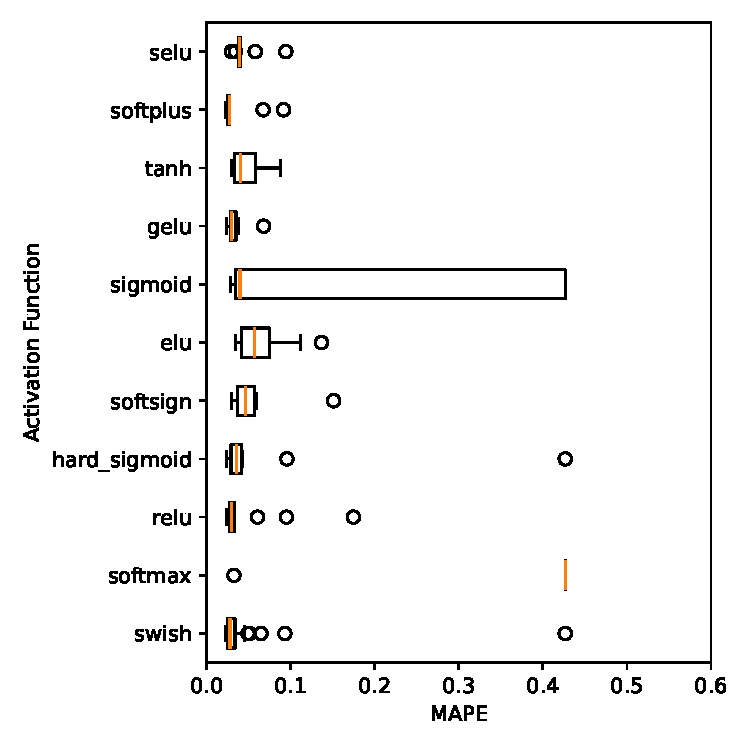
\includegraphics[width=\linewidth]{Figuras/hpo/hpo_plots_#1_#2/hpo_nn_activation_MAPE.pdf}  
        \caption{MAPE.}
        \label{fig:hpo_MAPE_a#1_#2}
    \end{subfigure}
    \begin{subfigure}{0.3\textwidth}
        \centering
        % include second image
        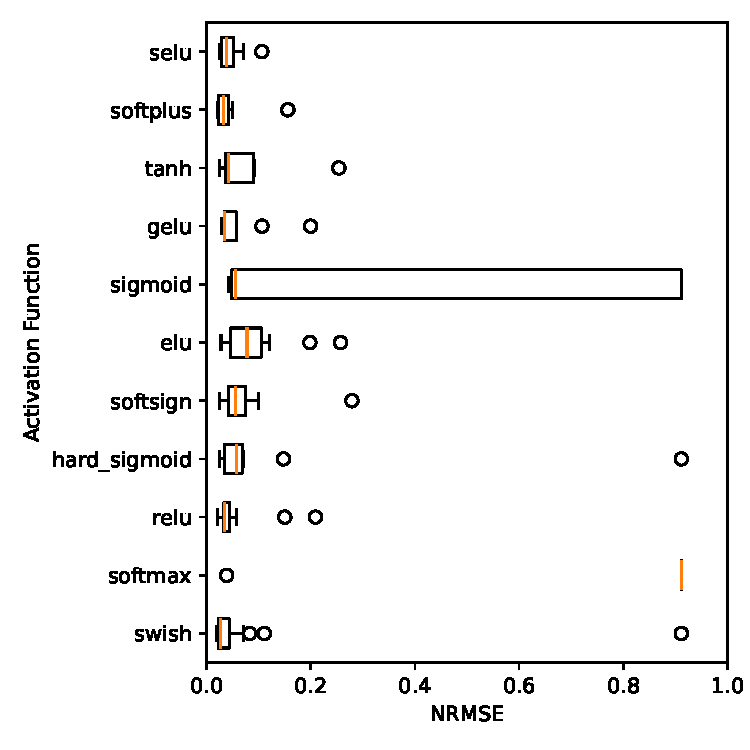
\includegraphics[width=\linewidth]{Figuras/hpo/hpo_plots_#1_#2/hpo_nn_activation_NRMSE.pdf}  
        \caption{NRMSE.}
        \label{fig:hpo_NRMSE_#1_#2}
    \end{subfigure}
    \begin{subfigure}{0.3\textwidth}
        \centering
        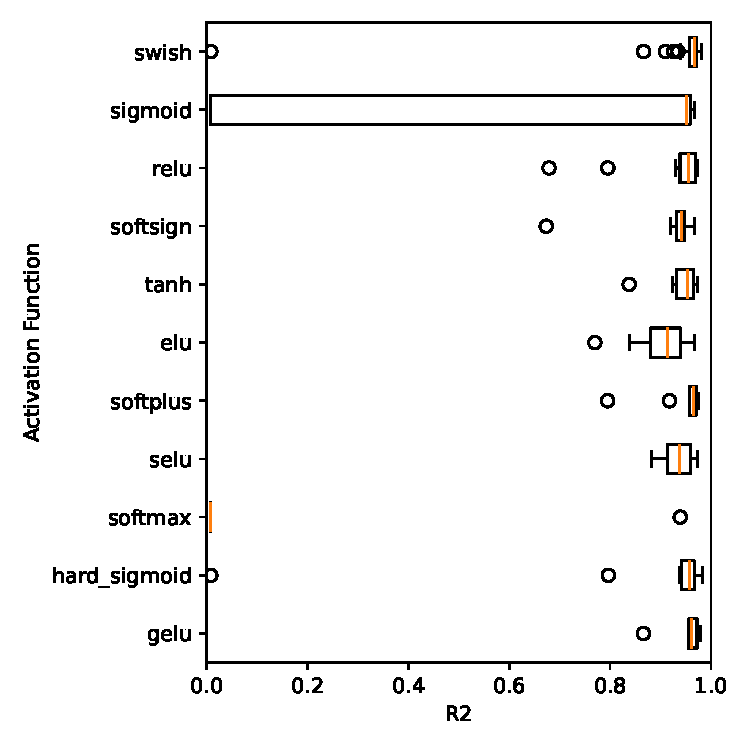
\includegraphics[width=\linewidth]{Figuras/hpo/hpo_plots_#1_#2/hpo_nn_activation_R2.pdf}  
        \caption{R2}
        \label{fig:hpo_R2_#1_#2}
    \end{subfigure}
    \caption{#3}
    \label{fig:hpo_#1_#2}
\end{figure}
}

\newcommand{\plothpomap}[3]{
\begin{figure}[t]
    \centering
    \begin{subfigure}{0.3\textwidth}
        \centering
        % include second image
        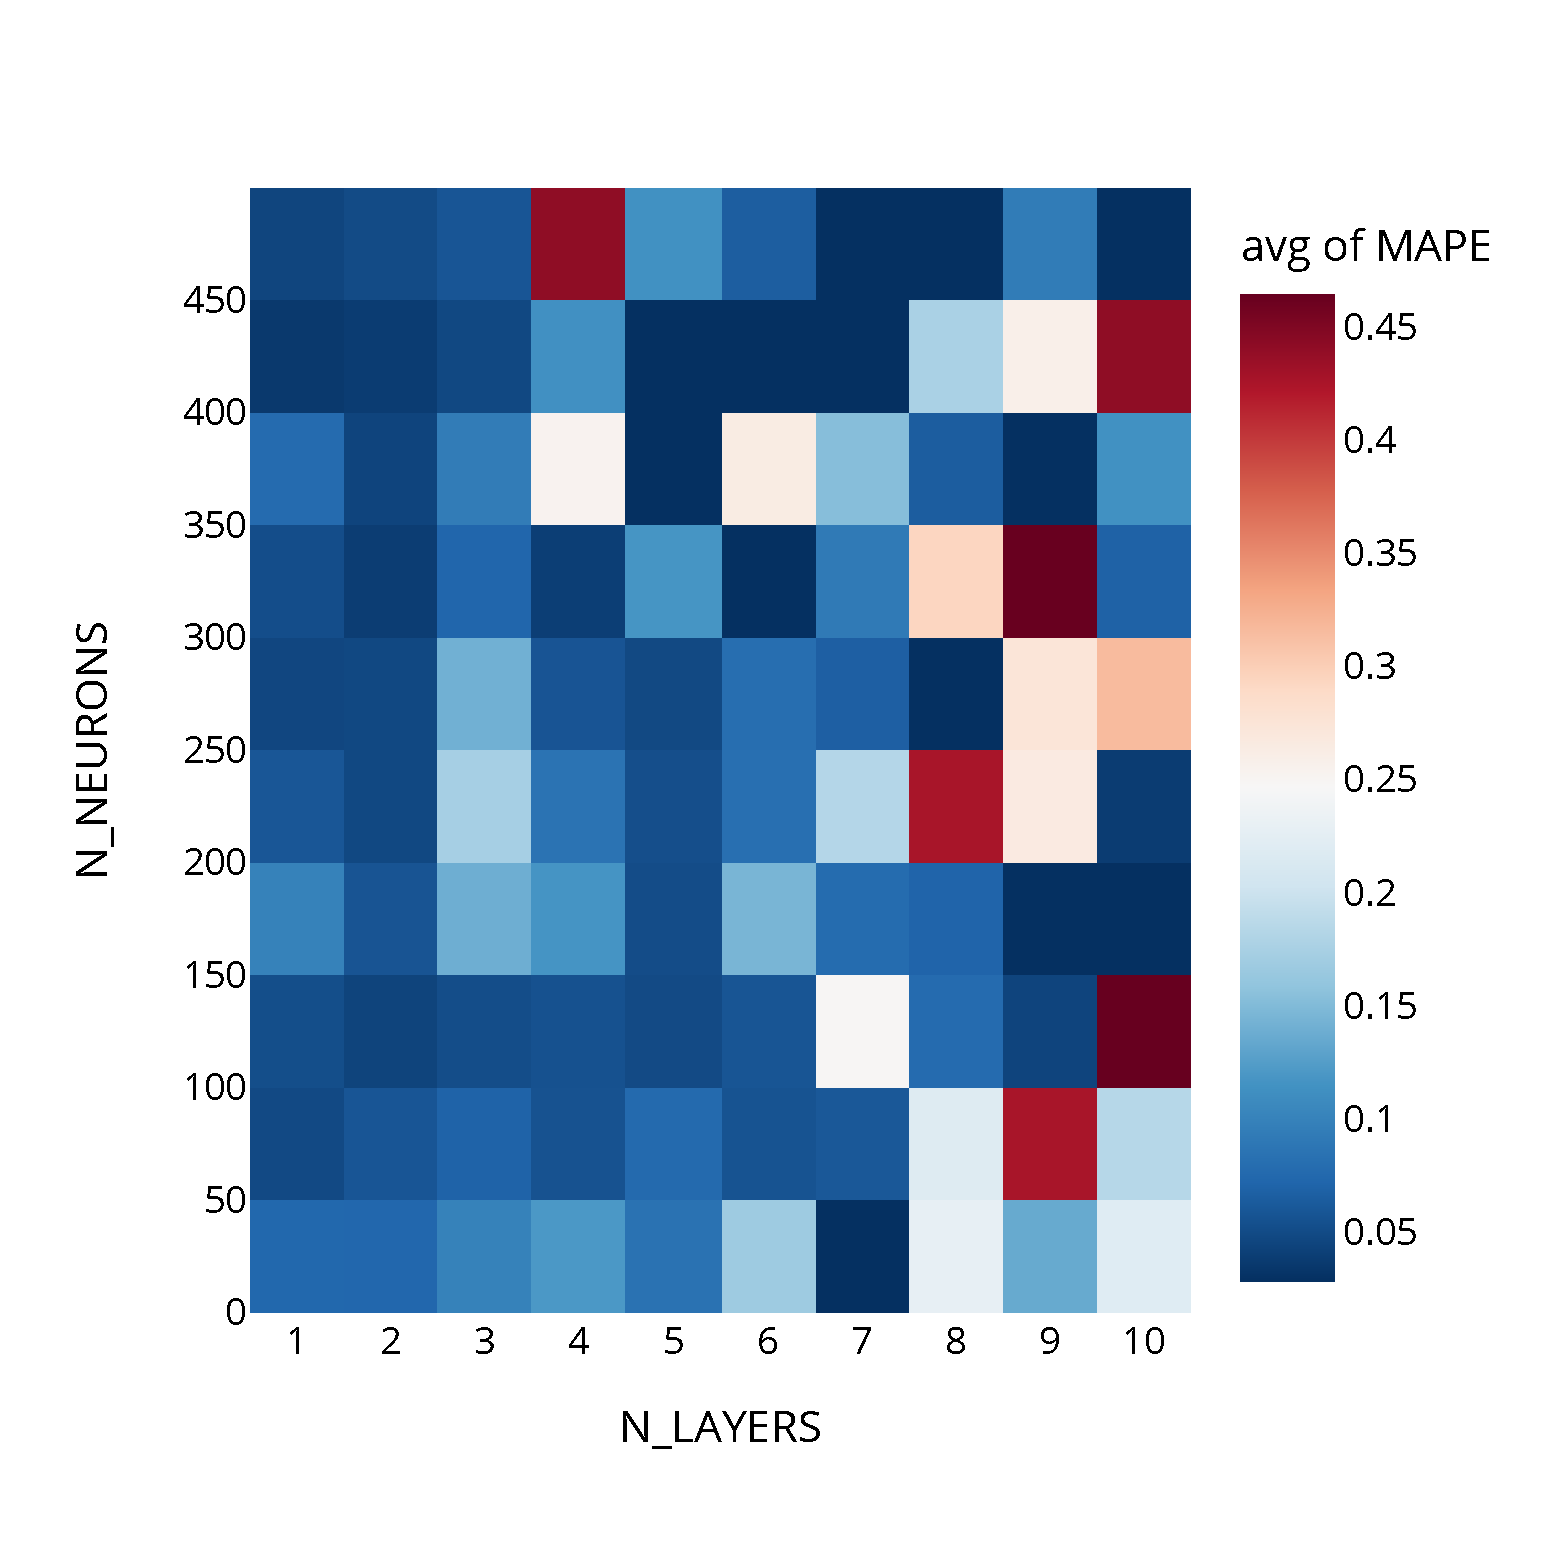
\includegraphics[width=\linewidth]{Figuras/hpo/hpo_plots_#1_#2/neurons_layers_heat_map_MAPE.pdf}  
        \caption{MAPE.}
        \label{fig:hpo_map_MAPE_all_all}
    \end{subfigure}
    \begin{subfigure}{0.3\textwidth}
        \centering
        % include second image
        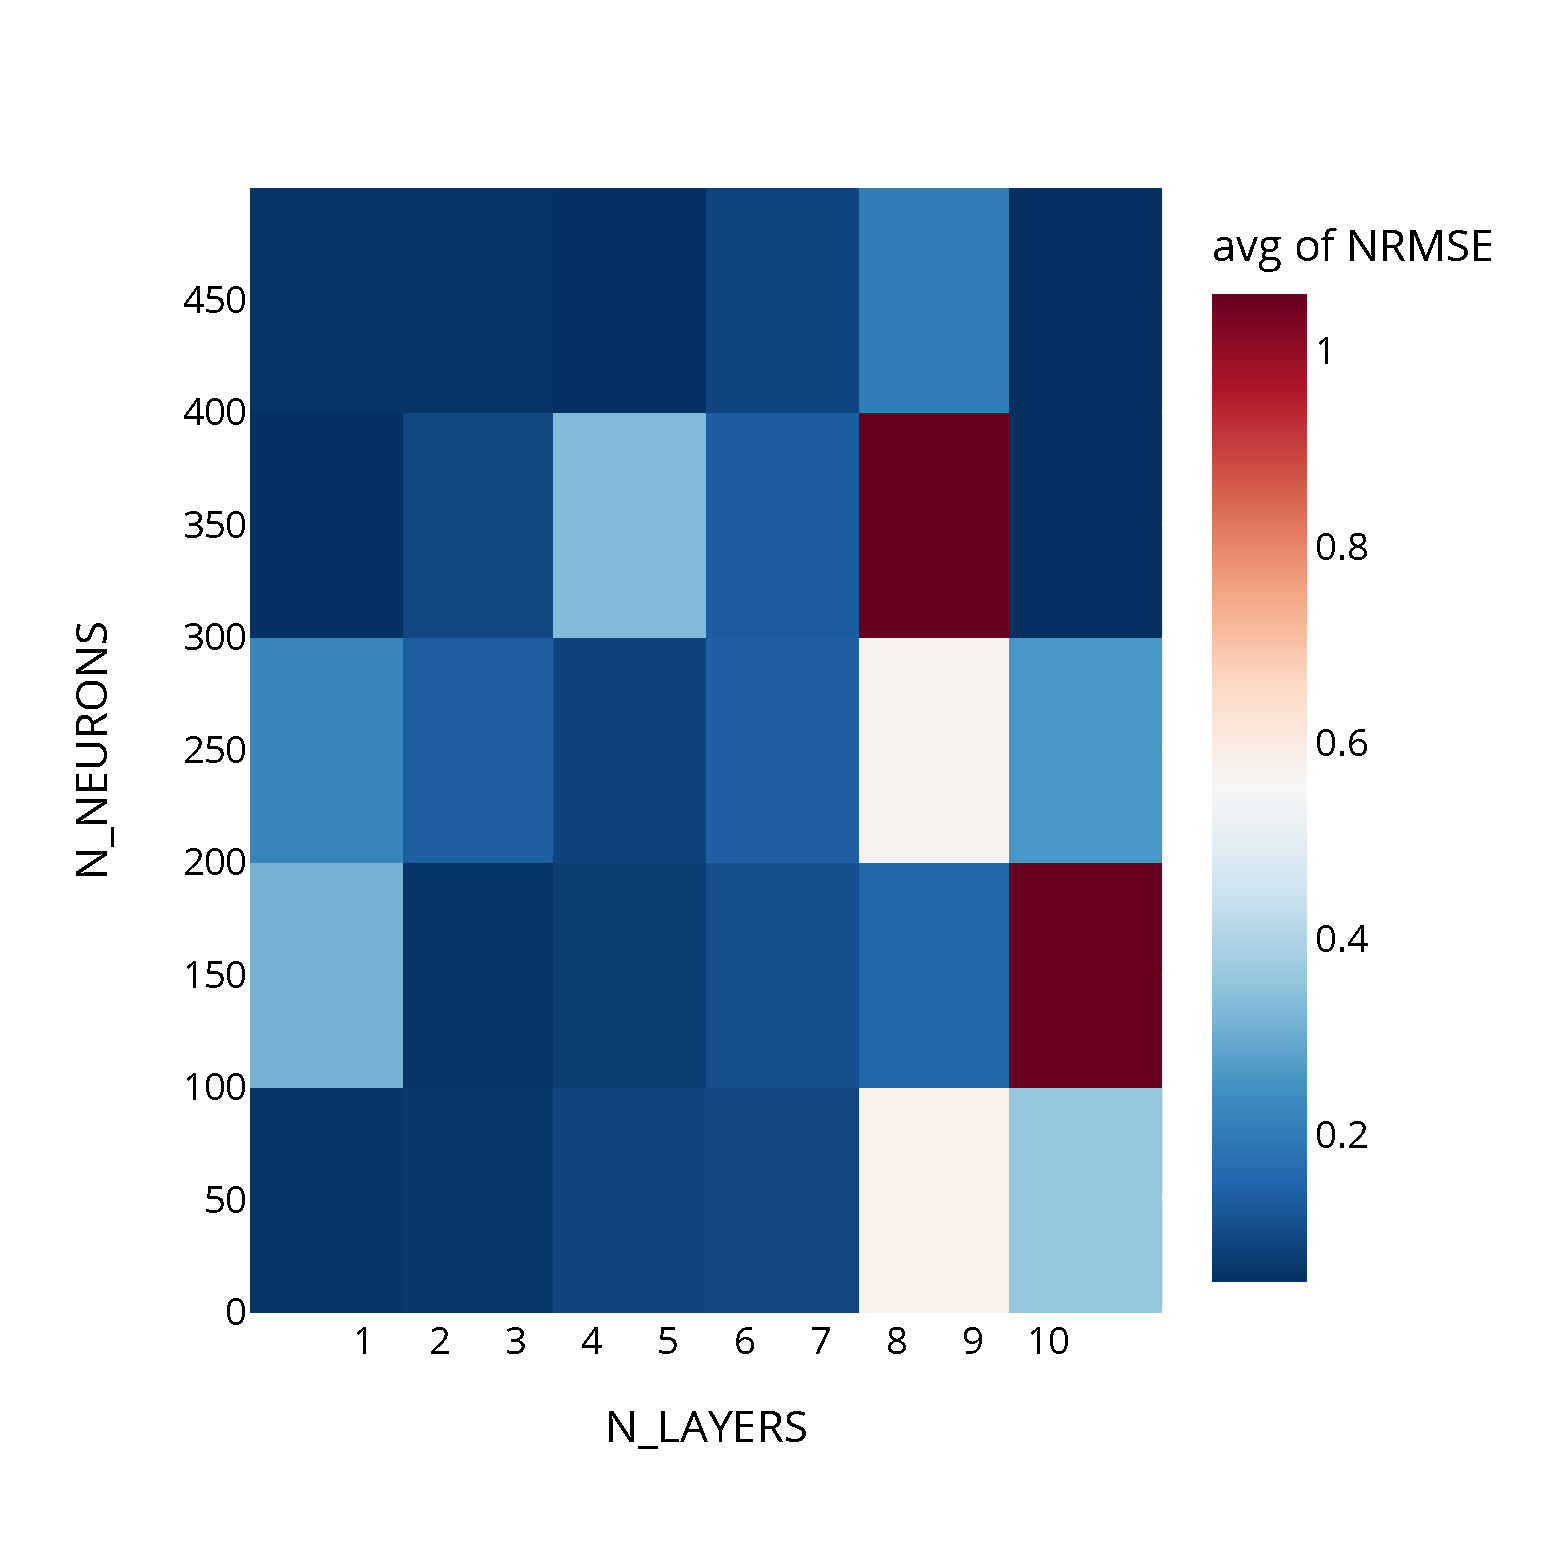
\includegraphics[width=\linewidth]{Figuras/hpo/hpo_plots_#1_#2/neurons_layers_heat_map_NRMSE.pdf}  
        \caption{NRMSE.}
        \label{fig:hpo_map_NRMSE_all_all}
    \end{subfigure}
    \begin{subfigure}{0.3\textwidth}
        \centering
        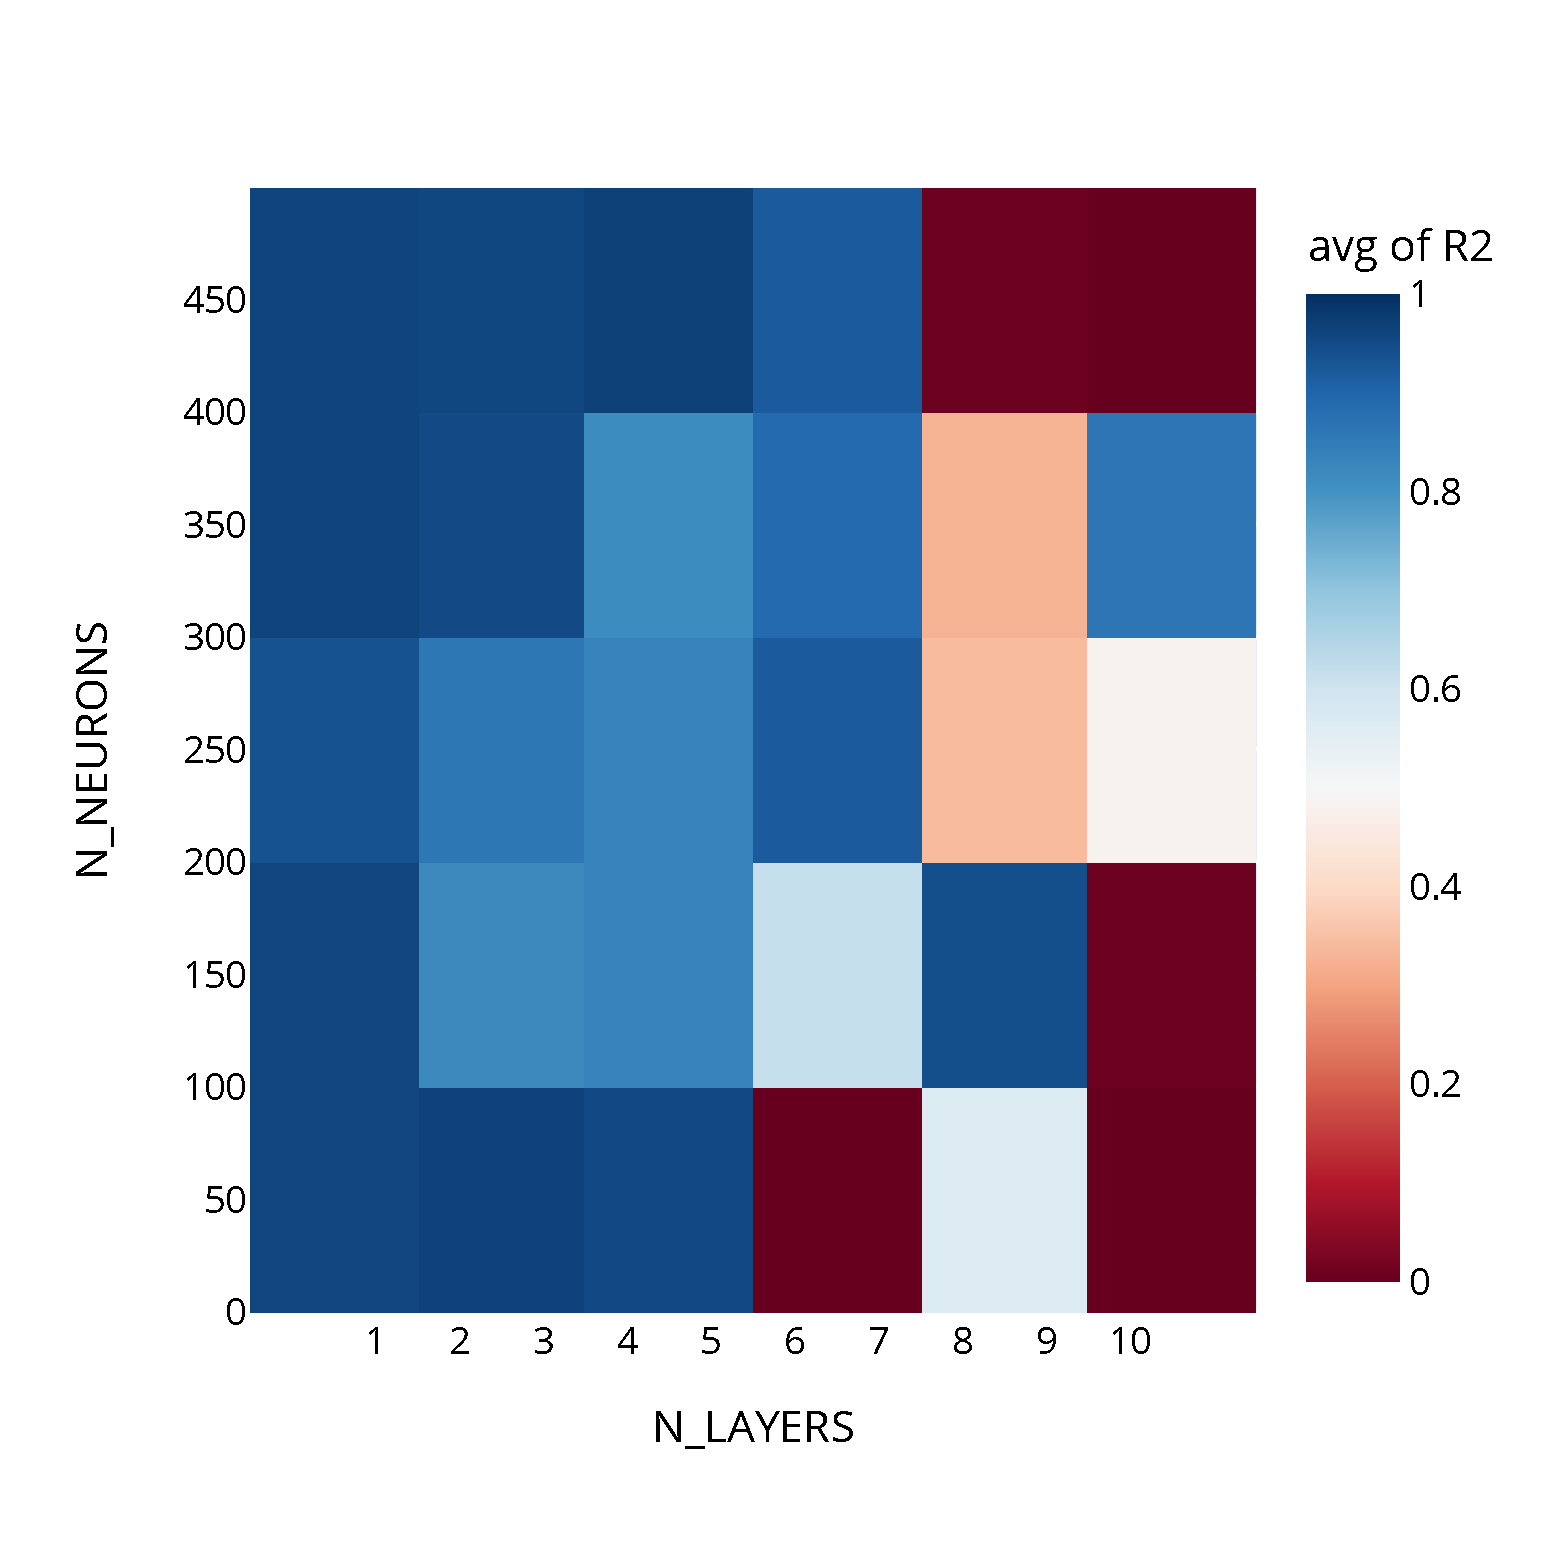
\includegraphics[width=\linewidth]{Figuras/hpo/hpo_plots_#1_#2/neurons_layers_heat_map_R2.pdf}  
        \caption{R2}
        \label{fig:hpo_map_R2_all_all}
    \end{subfigure}
    \caption{#3}
    \label{fig:hpo_map_all_all}
\end{figure}
}

\newcommand{\plothpohistogram}[3]{
\begin{figure}[t]
    \centering
    \begin{subfigure}{0.3\textwidth}
        \centering
        % include second image
        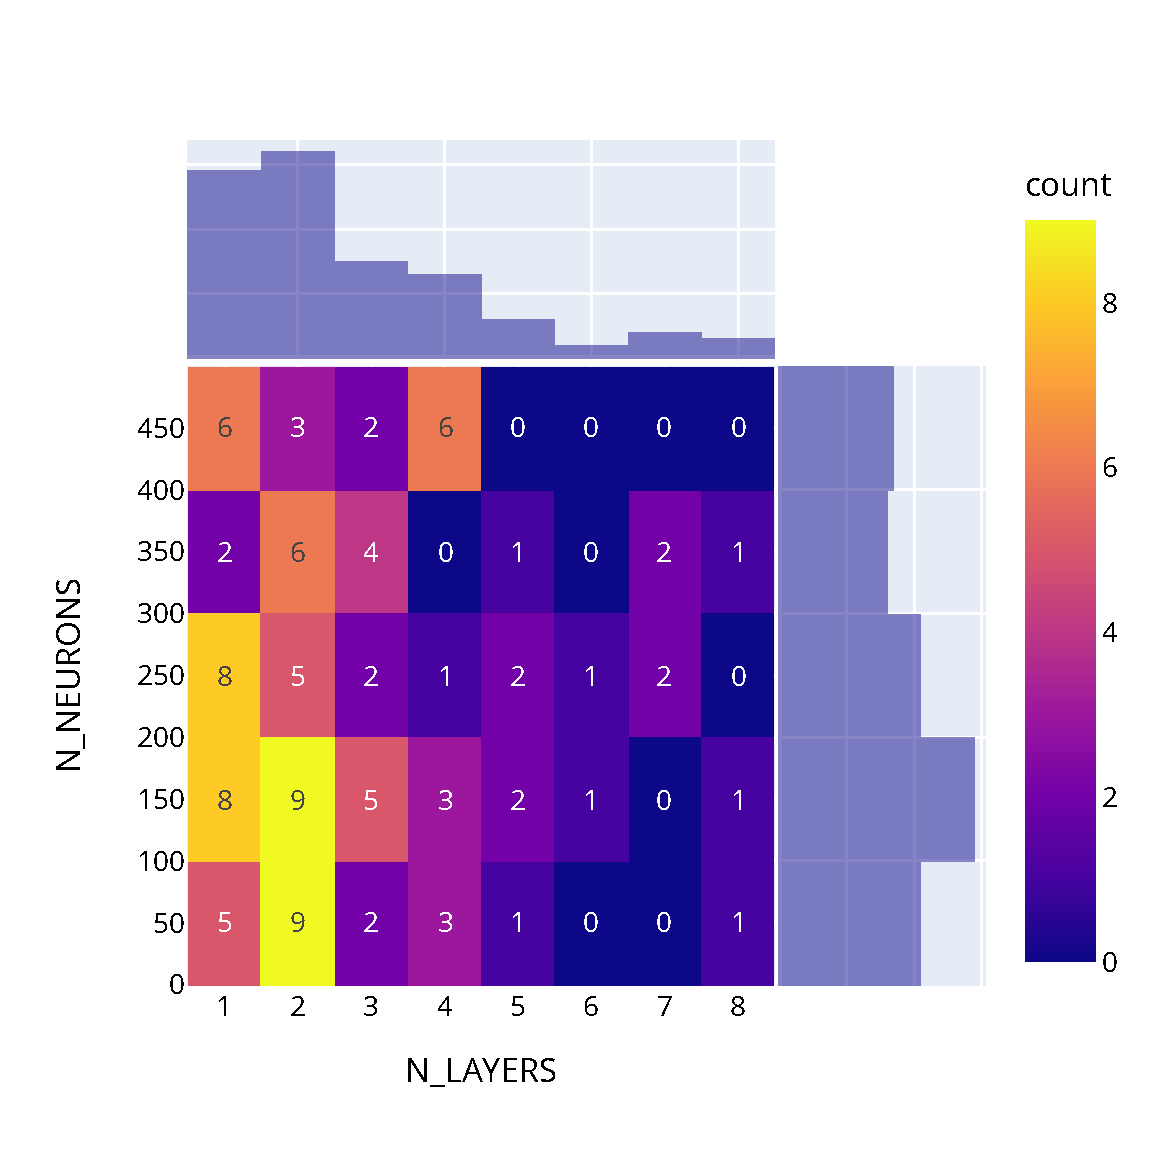
\includegraphics[width=\linewidth]{Figuras/hpo/hpo_plots_#1_#2/hpo_nn_hist_neurons_layers.pdf}  
        \caption{Histogram neurons layers.}
        \label{fig:hpo_hist_neurons_#1_#2}
    \end{subfigure}
    \begin{subfigure}{0.3\textwidth}
        \centering
        % include second image
        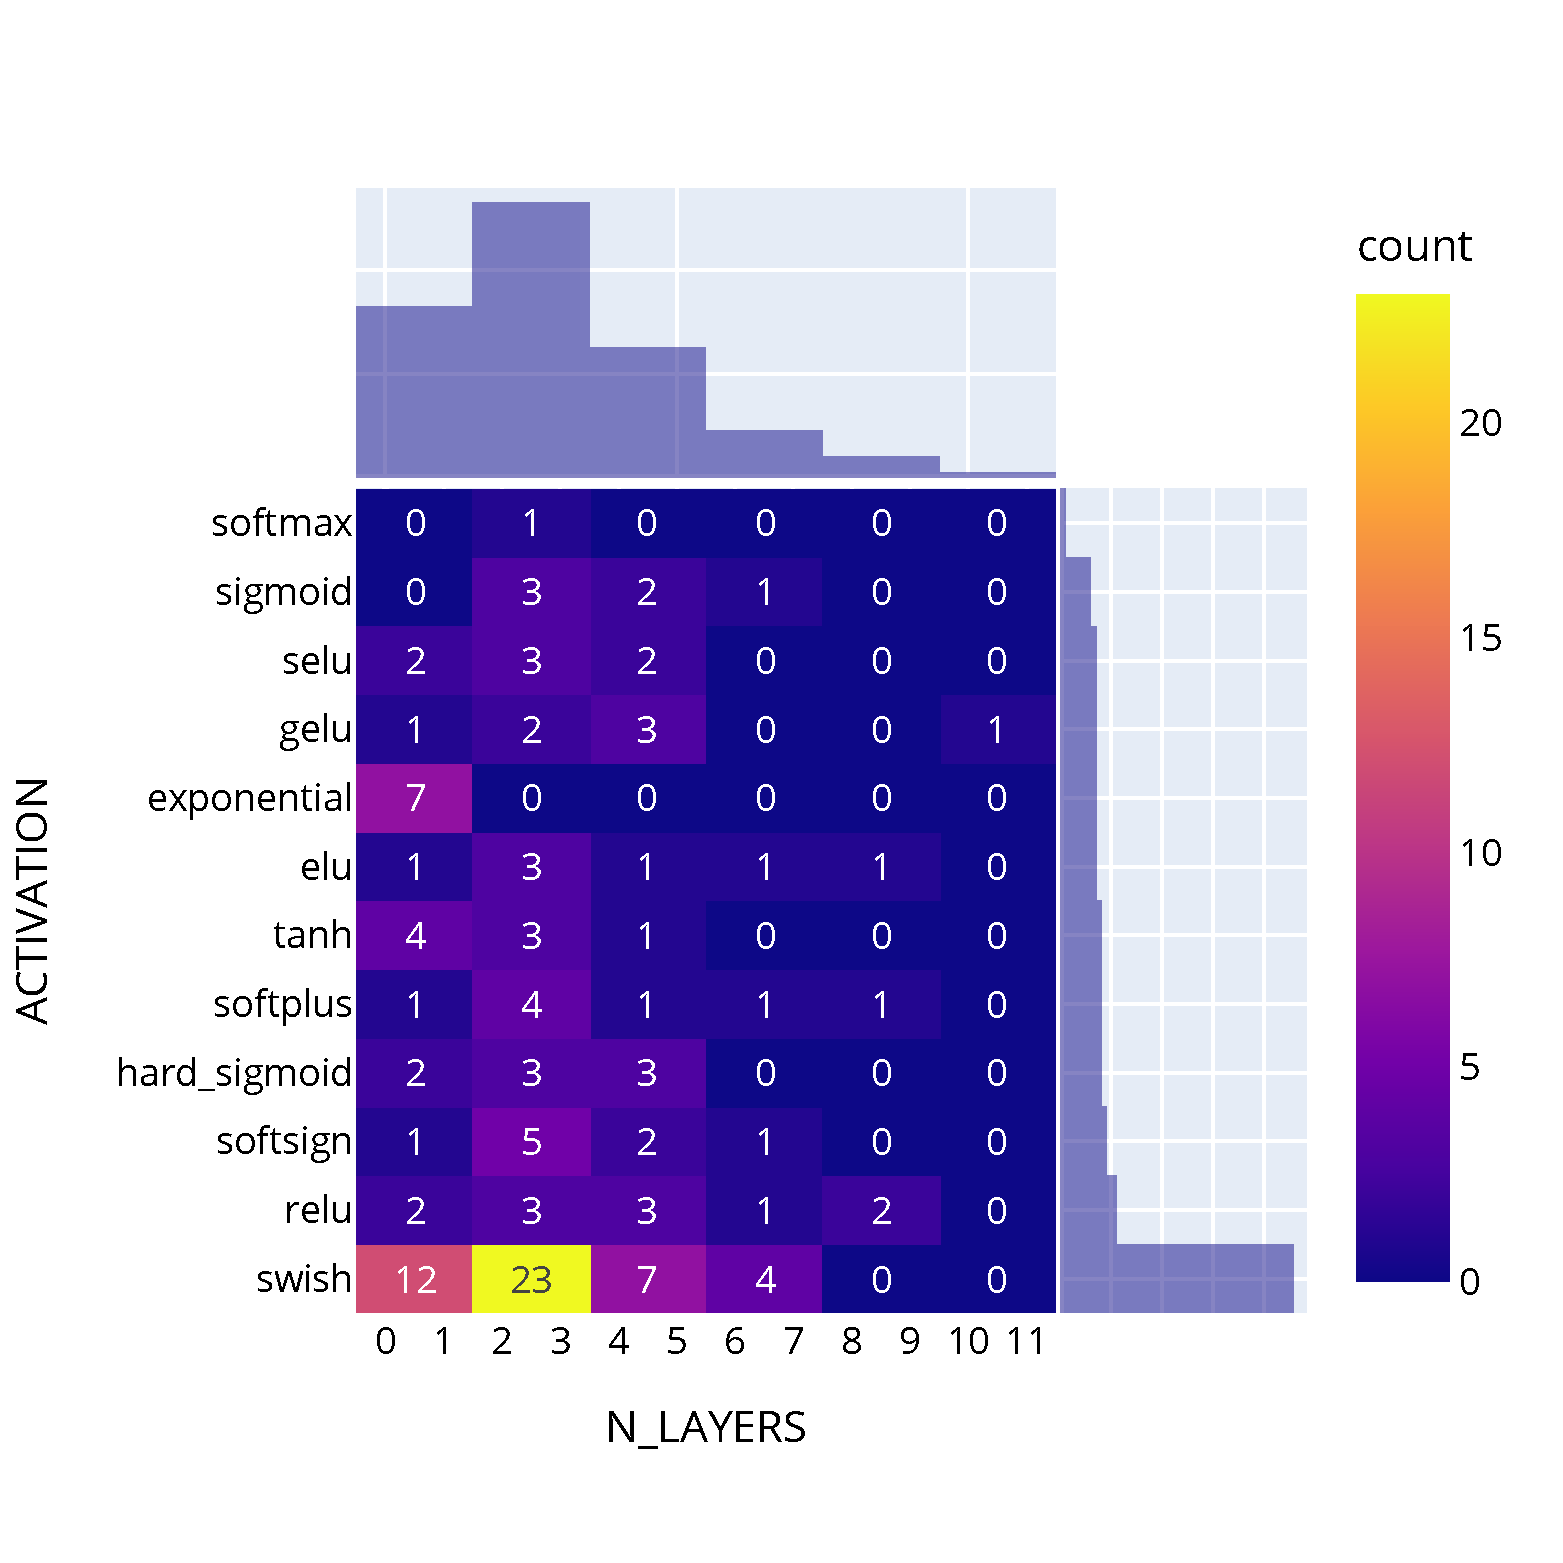
\includegraphics[width=\linewidth]{Figuras/hpo/hpo_plots_#1_#2/hpo_nn_activation_layers_count.pdf}  
        \caption{Histogram activation layers.}
        \label{fig:hpo_hist_activation_#1_#2}
    \end{subfigure}
    \begin{subfigure}{0.3\textwidth}
        \centering
        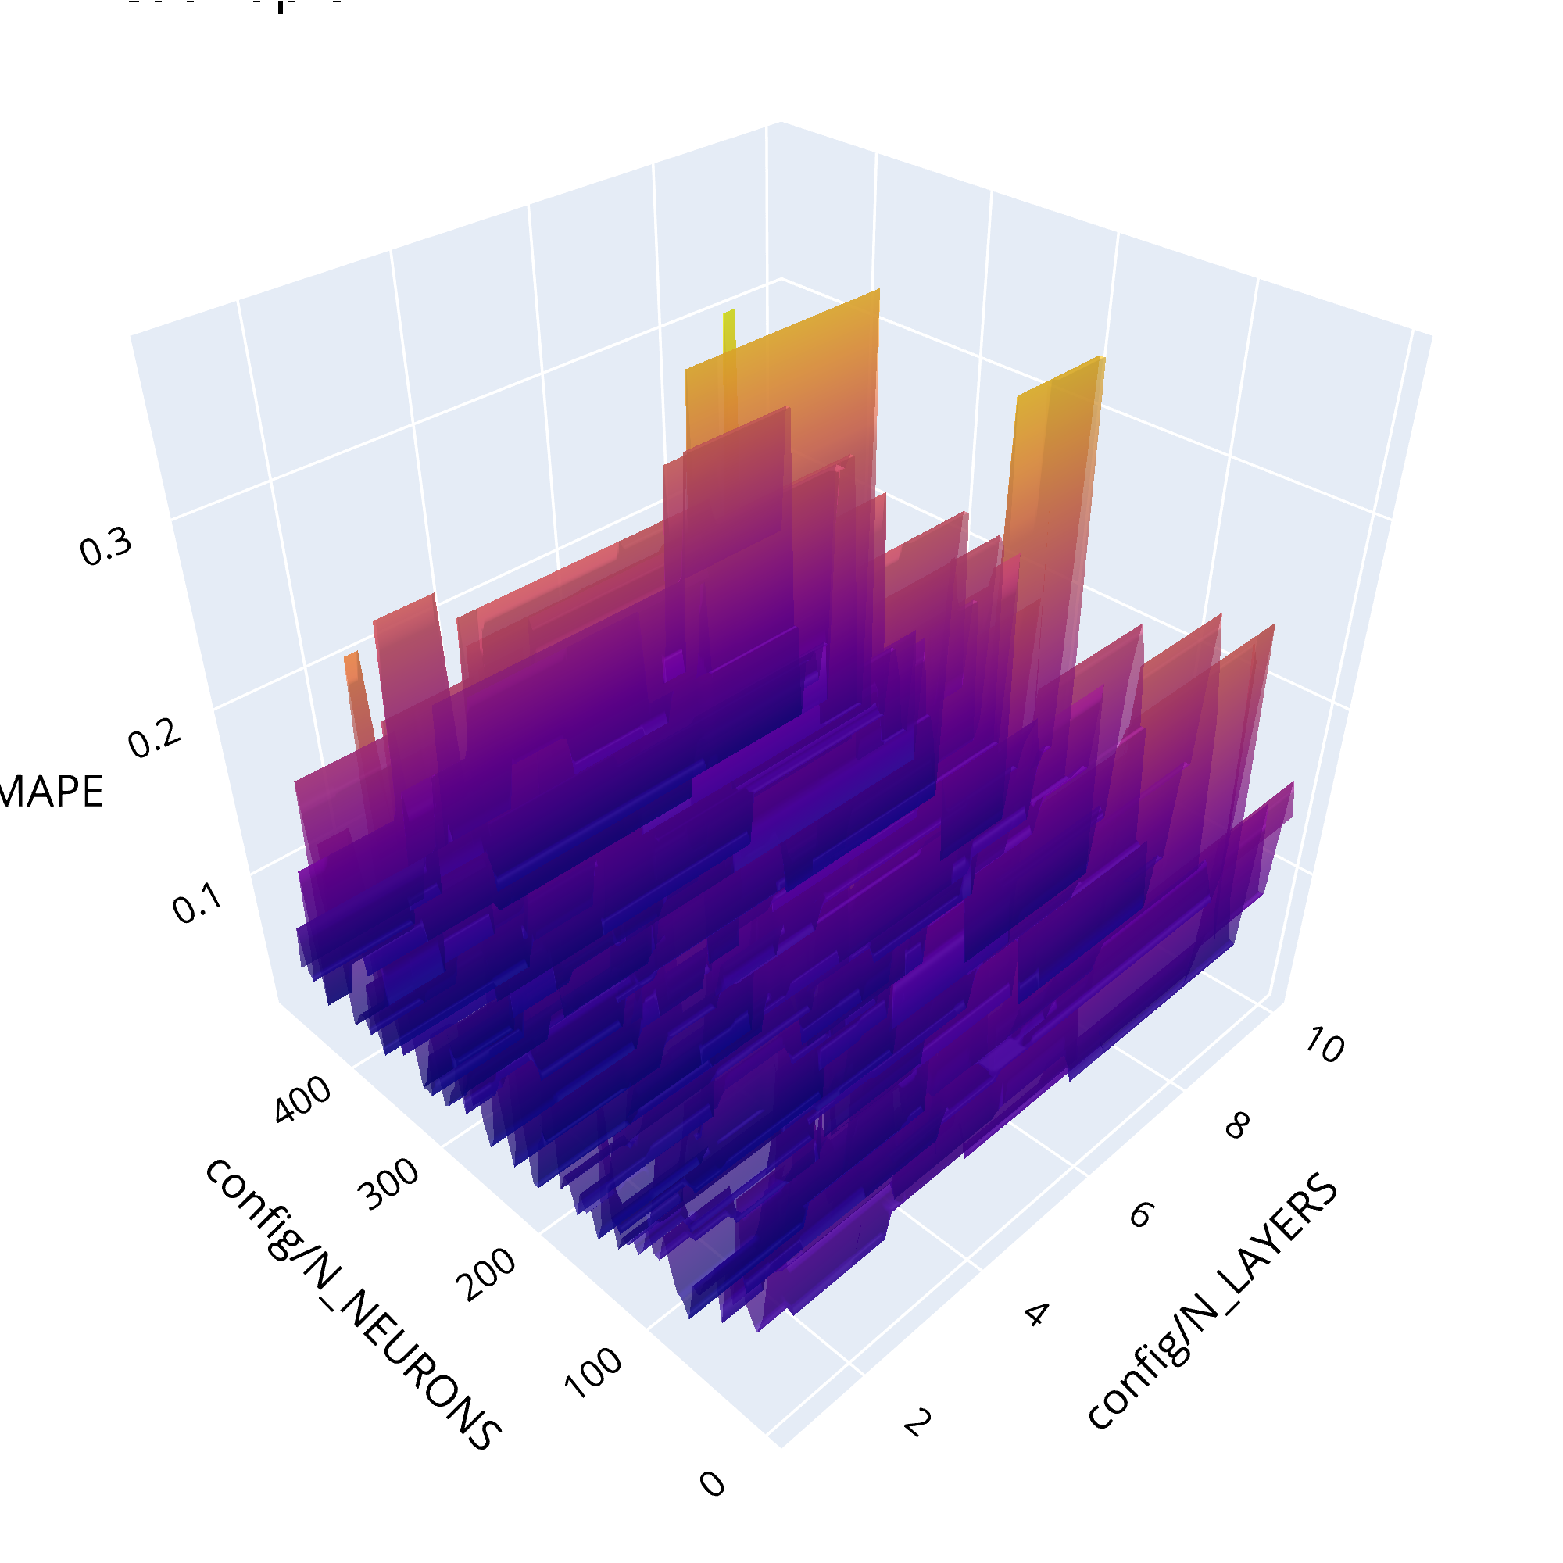
\includegraphics[width=\linewidth]{Figuras/hpo/hpo_plots_#1_#2/hpo_nn_activation_layers_surface.pdf}  
        \caption{Surface MAPE}
        \label{fig:hpo_surface_MAPE_#1_#2}
    \end{subfigure}
    \caption{#3}
    \label{fig:hpo_hist_#1_#2}
\end{figure}
}
%% =============================
%%      IMPORTANTE
%% ESTE ARQUIVO DEVE ESTAR SALVO COMO
%%      UTF - 8
%% =============================

% ----------------------------------------------------------
% Este capítulo é parte integrante do arquivo mestre
% Relatorio_TCC_Mestrado_Base_VERSÃO_SUBVERSÃO
% Formatos com \caption acima do \includegraphics conforme ABNT
% ----------------------------------------------------------

% -----------------------------------------
% Metodologia
%
% A ideia é utilizar a mesma sequência de entrada ter a opção de trocar a posição conforme a necessidade
% 
% O comando deve ser usado dentro do ambiente {figure} de forma que o comando \label{key} esteja dentro do ambiente e permita a melhor localização pelo editor LaTeX
%
% Forma de uso
%
% --------------------- Figuras Simples
%	\begin{figure}[H]
%		\figNameCommand{options includegraphics}{filename with path}{caption}
%		\label{label_figure_1}
%	\end{figure}
%
% --------------------- Figuras Compostas
%	\begin{figure}[H]
%		\figCapTwoSubfigInc{caption geral}
%		{subcaption (a) }
%		{width = 7cm, height = 6cm, trim = 0cm 0cm 0cm 0cm, clip = true}
%		{figure with path}
%		{subcaption (b) }
%		{width = 7cm, height = 6cm, trim = 0cm 0cm 0cm 0cm, clip = true}
%		{figure with path}
%		\label{fig_label}
%	\end{figure}
%
% --------------------- Comando Trim
% trim = left bottom right top
% -----------------------------------------

% -----------------------------------------
% Comandos para Figuras Simples
% -----------------------------------------
\newcommand{\figIncLongCap}[3]
{ 	
	\centering
	\caption{#3}
	\includegraphics[#1]{#2}
}

\newcommand{\figIncShortCap}[4]
{ 	
	\centering
	\caption[#4]{#3}
	\includegraphics[#1]{#2}
}

% -----------------------------------------
% Comandos para Figuras Duplas Com Subfigures
% -----------------------------------------
\newcommand{\figTwoSubfigIncLongCap}[7]
{ 	
	\centering
	\caption{#7}
	\subfigure[#1]
	{\includegraphics[#2]{#3}}
	\quad
	\subfigure[#4]
	{\includegraphics[#5]{#6}}
}

\newcommand{\figTwoSubfigIncShortCap}[8]
{ 	
	\centering
	\caption[#8]{#7}
	\subfigure[#1]
	{\includegraphics[#2]{#3}}
	\quad
	\subfigure[#4]
	{\includegraphics[#5]{#6}}
}

% -----------------------------------------
% Comandos para Figuras Triplas em Cascata Com Subfigures
% -----------------------------------------
\newcommand{\figThreeSubfigIncCap}[4]
{ 	
	\centering
	\SubfigSubcapSubfigInc{#1}
	\quad
	\SubfigSubcapSubfigInc{#2}
	\quad
	\SubfigSubcapSubfigInc{#3}
	\quad
	\caption{#4}
}

% -----------------------------------------
% Comandos Base para Figuras Múltiplas em Cascata Com Subfigures
% -----------------------------------------
\newcommand{\SubfigcapSubfigInc}[3]
{ 	
	\subfigure[#1]
	{\includegraphics[#2]{#3}} 
}

%%%%%%%%%%%%%%%%%%%%%%%%%%%%%%%%%%
% ===== Magno old versions ===== %
%%%%%%%%%%%%%%%%%%%%%%%%%%%%%%%%%%

% -----------------------------------------
% Comandos para Figuras Duplas sem Subfigure
% -----------------------------------------
\newcommand{\figDob}[5]
{   
	\centering
	\caption{#5}
	\includegraphics[#1]{#2}
	\includegraphics[#3]{#4} \\
	\vspace*{0.2cm}
	(a) \hspace{6.5cm} (b)
}

% -----------------------------------------
% Comandos para Figuras Triplas sem Subfigure
% -----------------------------------------
\newcommand{\figTre}[7]
{   
	\centering
	\caption{#7}
	\includegraphics[#1]{#2}
	\includegraphics[#3]{#4} \\
	\vspace*{0.2cm}
	(a) \hspace{6.5cm} (b) \\
	\includegraphics[#5]{#6} \\
	\vspace*{0.2cm}
	(c)
}

\newcommand{\figTreV}[7]
{   
	\centering
	\caption{#7}
	\includegraphics[#1]{#2}
	\includegraphics[#3]{#4}
	\includegraphics[#5]{#6}   \\
	\vspace*{0.2cm}
	(a) \hspace{4.cm} (b) \hspace{4.cm} (c)
}
% ----------------------------------------------------------
% Fim Arquivo
%%% =============================
%%      IMPORTANTE
%% ESTE ARQUIVO DEVE ESTAR SALVO COMO
%%      UTF - 8
%% =============================

% ----------------------------------------------------------
% Este capítulo é parte integrante do arquivo mestre
% Relatorio_TCC_Mestrado_Base_VERSÃO_SUBVERSÃO
% Formatos com \caption acima do \includegraphics conforme todos exceto ABNT, e.g., IEEE
% ----------------------------------------------------------

% -----------------------------------------
% Metodologia
%
% A ideia é utilizar a mesma sequência de entrada ter a opção de trocar a posição conforme a necessidade
% 
% O comando deve ser usado dentro do ambiente {figure} de forma que o comando \label{key} esteja dentro do ambiente e permita a melhor localização pelo editor LaTeX
%
% Forma de uso
%
% --------------------- Figuras Simples
%	\begin{figure}[H]
%		\figNameCommand{options includegraphics}{filename with path}{caption}
%		\label{label_figure_1}
%	\end{figure}
%
% --------------------- Figuras Compostas
%	\begin{figure}[H]
%		\figCapTwoSubfigInc{caption geral}
%		{subcaption (a) }
%		{width = 7cm, height = 6cm, trim = 0cm 0cm 0cm 0cm, clip = true}
%		{figure with path}
%		{subcaption (b) }
%		{width = 7cm, height = 6cm, trim = 0cm 0cm 0cm 0cm, clip = true}
%		{figure with path}
%		\label{fig_label}
%	\end{figure}
%
% --------------------- Comando Trim
% trim = left bottom right top
% -----------------------------------------

% -----------------------------------------
% Comandos para Figuras Simples
% -----------------------------------------
\newcommand{\figIncLongCap}[3]
{ 	
	\centering
	\includegraphics[#1]{#2}
	\caption{#3}
}

\newcommand{\figIncShortCap}[4]
{ 	
	\centering
	\includegraphics[#1]{#2}
	\caption[#4]{#3}
}

% -----------------------------------------
% Comandos para Figuras Duplas Com Subfigures
% -----------------------------------------
\newcommand{\figTwoSubfigIncLongCap}[7]
{ 	
	\centering
	\subfigure[#1]
	{\includegraphics[#2]{#3}}
	\quad
	\subfigure[#4]
	{\includegraphics[#5]{#6}}
	\caption{#7}
}

\newcommand{\figTwoSubfigIncShortCap}[8]
{ 	
	\centering
	\subfigure[#1]
	{\includegraphics[#2]{#3}}
	\quad
	\subfigure[#4]
	{\includegraphics[#5]{#6}}
	\caption[#8]{#7}
}

% -----------------------------------------
% Comandos para Figuras Triplas em Cascata Com Subfigures
% -----------------------------------------
\newcommand{\figThreeSubfigIncCap}[4]
{ 	
	\centering
	\SubfigSubcapSubfigInc{#1}
	\quad
	\SubfigSubcapSubfigInc{#2}
	\quad
	\SubfigSubcapSubfigInc{#3}
	\quad
	\caption{#4}
}

% -----------------------------------------
% Comandos Base para Figuras Múltiplas em Cascata Com Subfigures
% -----------------------------------------
\newcommand{\SubfigcapSubfigInc}[3]
{ 	
	\subfigure[#1]
	{\includegraphics[#2]{#3}} 
}

%%%%%%%%%%%%%%%%%%%%%%%%%%%%%%%%%%
% ===== Magno old versions ===== %
%%%%%%%%%%%%%%%%%%%%%%%%%%%%%%%%%%

% -----------------------------------------
% Comandos para Figuras Duplas sem Subfigure
% -----------------------------------------
\newcommand{\figDob}[5]
{   
	\centering
	\includegraphics[#1]{#2}
	\includegraphics[#3]{#4} \\
	\vspace*{0.2cm}
	(a) \hspace{6.5cm} (b) %\\
	\caption{#5}
}

% -----------------------------------------
% Comandos para Figuras Triplas sem Subfigure
% -----------------------------------------
\newcommand{\figTre}[7]
{   
	\centering
	\includegraphics[#1]{#2}
	\includegraphics[#3]{#4} \\
	\vspace*{0.2cm}
	(a) \hspace{6.5cm} (b) \\
	\includegraphics[#5]{#6} \\
	\vspace*{0.2cm}
	(c)
	\caption{#7}
}

\newcommand{\figTreV}[7]
{   
	\centering
	\includegraphics[#1]{#2}
	\includegraphics[#3]{#4}
	\includegraphics[#5]{#6}   \\
	\vspace*{0.2cm}
	(a) \hspace{4.cm} (b) \hspace{4.cm} (c)
	\caption{#7}
}
% ----------------------------------------------------------
% Fim Arquivo

% ==========

% ==========  Seleção de uso de links coloridos para visualização ou sem cor para impressão final
%\toggletrue{LinksComCores} 		% Opção links COM CORES => Forma para auxiliar na escrita do relatório
\togglefalse{LinksComCores} 		% Opção links SEM CORES => Forma correta para imprimir a versão final a ser entregue
% ==========

% ========== Pacotes
%% =============================
%%      IMPORTANTE
%% ESTE ARQUIVO DEVE ESTAR SALVO COMO
%%      UTF - 8
%% =============================

% ----------------------------------------------------------
% Este capítulo é parte integrante do arquivo mestre
% Relatorio_TCC_Mestrado_Base_VERSÃO_SUBVERSÃO
% ----------------------------------------------------------
\usepackage{natbib}
\usepackage[T1]{fontenc}
%\usepackage[latin1]{inputenc}
\usepackage[utf8]{inputenc}
% =========
\usepackage{pgfplots}
\usepackage{tabularx}
% -----------------------------------------
% Pacotes básicos 
% -----------------------------------------
\usepackage[section]{placeins}
\usepackage{lastpage}		% Usado pela Ficha catalográfica
\usepackage{indentfirst}	% Indenta o primeiro parágrafo de cada seção.
\usepackage{color}			% Controle das cores
\usepackage{microtype} 		% Melhorias de justificação \usepackage[section]{placeins}
% \usepackage{amsmath} 		% Referências de equações com parênteses automático usar \eqref
\usepackage{physics,amsmath}

\usepackage{amssymb} 		% Símbolos matemáticos, incluindo os principais conjuntos numéricos
\usepackage{cancel}
% -----------------------------------------

% -----------------------------------------
% Pacotes gráficos
% -----------------------------------------
\usepackage{ae}
\usepackage{aecompl}
\usepackage{graphicx, import}	% Inclusão de gráficos
\usepackage{float} 		% Permite que eu use "H" para a figura ficar entre os parágrafos que eu quero
%\usepackage{subfigure} % make it possible to include more than one captioned figure/table in a single float
%\usepackage[font=small,labelfont=bf]{caption}
\usepackage[font=footnotesize]{caption} % Reduz o tamanho de todos os ``captions''
%\usepackage{subcaption}
%\usepackage{subfloat} % make it possible to include more than one captioned 
\usepackage{epstopdf}
\usepackage{ulem}
\usepackage{nomencl}
\makenomenclature
% \usepackage{framed}
\usepackage{lipsum} % geração de texto inútil - dummy
\usepackage{morefloats}

% -----------------------------------------
% Pacotes gráficos - Formatação do título
% -----------------------------------------
% Se fncychap for adicionado como RequirePackage dentro de ufabcFHZ#.cls não gera o mesmo efeito.
\usepackage[Bjornstrup]{fncychap} % Formas elegantes de cabeçalho
%% ------------------------------------
% Referência: http://tex.stackexchange.com/questions/13357/fncychap-package-reduce-vertical-gap-space-between-header-and-chapter-heading
%% ------------------------------------
%% A única alteração feita é em ``\vspace'', por padrão será usado ``-1cm'', fica bom, maximiza o espaço  - Não é necessário editar esse trecho.
%% ------------------------------------
\makeatletter
\renewcommand*{\@makechapterhead}[1]{%
	%\vspace*{-5\p@}%
	\vspace*{-1cm}% Recuo vertical para maximizar aproveitamento da página
	{\parindent \z@ \raggedright \normalfont
		\ifnum \c@secnumdepth >\m@ne
		\if@mainmatter%%%%% Fix for frontmatter, mainmatter, and backmatter 040920
		\DOCH
		\fi
		\fi
		\interlinepenalty\@M
		\if@mainmatter%%%%% Fix for frontmatter, mainmatter, and backmatter 060424
		\DOTI{#1}%
		\else%
		\DOTIS{#1}%
		\fi
	}
}
% For the case \chapter*:
\renewcommand*{\@makeschapterhead}[1]{%
	\vspace*{-1cm}% Recuo vertical para maximizar aproveitamento da página
	{\parindent \z@ \raggedright
		\normalfont
		\interlinepenalty\@M
		\DOTIS{#1}
		\vskip 40\p@
	}
}
\makeatother
%% ------------------------------------

% -----------------------------------------
% Pacotes Ambiente de comentário
% -----------------------------------------
\usepackage{comment}

% ----------------------------------------- 
% Tabelas
% ----------------------------------------- 
\usepackage{booktabs} % for much better looking tables
\usepackage{multirow} % Permite uma célula de várias linhas
% ----------------------------------------- 

% ----------------------------------------- 
% Enumerate com letras pré-fixas
% ----------------------------------------- 
\usepackage{paralist} 		% very flexible & customisable lists (eg. enumerate/itemize, etc.)
\usepackage{enumitem}

% ----------------------------------------- 
% Equações
% ----------------------------------------- 
\usepackage{breqn} 		 % Garante quebra automático com \begin{dmath}, mesmo contador de \begin{equation}
\usepackage{array} 		 % for better arrays (eg matrices) in maths
\usepackage{subeqnarray} % Permite o use de subnumeração numa equação 1.a 1.b 1.c etc
\usepackage{cancel} 	 % Permite o corte numa simplificação de expressão:
% \cancel{expression}
% \cancelto{value}{expression}

% ----------------------------------------- 
% Links Coloridos - Com seleção de uso de cores pelo usuário no arquivo base usando \toogletrue ou \togglefalse
% ----------------------------------------- 
\usepackage[colorlinks=true,
linkcolor 		= red,
anchorcolor 	= black,
citecolor 		= green,
filecolor 		= cyan,
	% ==== Selecionando opção de links coloridos - Em parceria com comando "\newtoggle{LinksComCores}"
	\iftoggle{LinksComCores}{%
		%hidelinks
	}{%
		hidelinks
	}
	% ==== 
]{hyperref} %Pacote para hyperlinks
%hidelinks %opção para os links não serem coloridos, útil para a versão final do trabalho, também posso usar %linkcolor=black


% ----------------------------------------- 
% Links Coloridos - Com seleção de uso de cores (des)comentando "hidelinks"
%% - Este código está dentro da classe ufabcFHZ#.cls
%% - 	Ele é mantido aqui para conferência
% ----------------------------------------- 
%\usepackage[colorlinks=true,
%linkcolor 		= red,
%anchorcolor 	= black,
%citecolor 		= green,
%filecolor 		= cyan,
%hidelinks
%]{hyperref} %Pacote para hyperlinks
%%hidelinks %opção para os links não serem coloridos, útil para a versão final do trabalho, também posso usar %linkcolor=black

% ----------------------------------------- 
% Inserção de código do Matlab
% ----------------------------------------- 
\usepackage[numbered]{mcode} 		% configure listings for Matlab

%==== Pacote para url nas referências da ABNT
%\usepackage[num,abnt-url-package=url]{abntcite}
%====

% for subfigures
\usepackage{caption}
\usepackage{subcaption}
\usepackage{capt-of}

% to draw circuits
\usepackage{circuitikz}
\usepackage{tikz}

\usepackage{makecell}
% ----------------------------------------------------------
% Fim Arquivo

\usetikzlibrary{shapes.geometric,arrows.meta}
\usetikzlibrary{positioning}
\usetikzlibrary{calc}
\usetikzlibrary{backgrounds}
\usetikzlibrary{fit}

\tikzstyle{diam} = [diamond, aspect=2, draw, fill=red!40, text width=6em,text centered ]
\tikzstyle{block} = [rectangle, draw, fill=blue!20, text width=3cm,text centered, rounded corners, minimum height=2em ]
\tikzstyle{trap} = [trapezium, trapezium left angle=70, trapezium right angle=110, minimum height=2em, text centered, draw=red, fill=green!30]
\tikzstyle{rect} = [rectangle, minimum width=3cm, minimum height=1cm, text centered, draw=red, fill=orange!30]
\tikzstyle{line} = [draw, -latex]


% for pseudo codes
\usepackage{algorithm}
\usepackage[noend]{algpseudocode}

\makeatletter
\newcommand*{\algrule}[1][\algorithmicindent]{%
  \makebox[#1][l]{%
    \hspace*{.2em}% <------------- This is where the rule starts from
    \vrule height .75\baselineskip depth .25\baselineskip
  }
}
\newcount\ALG@printindent@tempcnta
\def\ALG@printindent{%
    \ifnum \theALG@nested>0% is there anything to print
    \ifx\ALG@text\ALG@x@notext% is this an end group without any text?
    % do nothing
    \else
    \unskip
    % draw a rule for each indent level
    \ALG@printindent@tempcnta=1
    \loop
    \algrule[\csname ALG@ind@\the\ALG@printindent@tempcnta\endcsname]%
    \advance \ALG@printindent@tempcnta 1
    \ifnum \ALG@printindent@tempcnta<\numexpr\theALG@nested+1\relax
    \repeat
    \fi
    \fi
}
% the following line injects our new indent handling code in place of the default spacing
\patchcmd{\ALG@doentity}{\noindent\hskip\ALG@tlm}{\ALG@printindent}{}{\errmessage{failed to patch}}
\patchcmd{\ALG@doentity}{\item[]\nointerlineskip}{}{}{} % no spurious vertical space
% end vertical rule patch for algorithmicx
\makeatother

% mathcal lowerletters
%\usepackage{dutchcal}

%\input{Pacotes/Input_Pacotes_for_IEEE}
%% =============================
%%      IMPORTANTE
%% ESTE ARQUIVO DEVE ESTAR SALVO COMO
%%      UTF - 8
%% =============================

% ----------------------------------------------------------
% Este capítulo é parte integrante do arquivo mestre
% Relatorio_TCC_Mestrado_Base_VERSÃO_SUBVERSÃO
% ----------------------------------------------------------


%================ Pacotes para inserir código
% ----------------------------------------- 
% Inserção de código do Matlab
% ----------------------------------------- 
\usepackage[numbered]{mcode} 		% configure listings for Matlab

% Deve estar na mesma pasta que o arquivo Base do relatório
%%%% *** Bloco adicionado em mcode.sty - FHZ
% % general definitions
% \lstset{%
% extendedchars = true,
% inputencoding = latin1, % funciona com latin1
%%%% ***

% ----------------------------------------- 
% en­ables the user to type­set pro­grams (pro­gram­ming code) 
% ----------------------------------------- 
\usepackage{listings}

%%%%% ++++++ Referências e explicações:
%http://tex.stackexchange.com/questions/68356/how-to-create-conditionals-in-a-document-class-for-latex
%http://tex.stackexchange.com/questions/30512/how-to-insert-code-with-accents-with-listings
%http://tex.stackexchange.com/questions/24528/having-problems-with-listings-and-utf-8-can-it-be-fixed
%http://tex.stackexchange.com/questions/30512/how-to-insert-code-with-accents-with-listings
%http://tex.searchalleasy.com/q/30512
%http://stackoverflow.com/questions/1116266/listings-in-latex-with-utf-8-or-at-least-german-umlauts
%http://www.mathworks.com/matlabcentral/fileexchange/8015-m-code-latex-package
%%%%% ++++++ 

% ----------------------------------------- 
% --- Comando para definir estilo da \lstinputlisting
% ----------------------------------------- 
\lstset{basicstyle=\footnotesize}

% ----------------------------------------- 
% --- Comando para garantir acentuação correta para \lstinputlisting[language = C].
% ----------------------------------------- 
\lstset{literate = %
	{Ö}{{\"O}}1
	{Ä}{{\"A}}1
	{Ü}{{\"U}}1
	{ß}{{\s{s}}}1
	{ü}{{\"u}}1
	{ä}{{\"a}}1
	{ö}{{\"o}}1
	{~}{{\textasciitilde}}1
	{ã}{{\~a}}1
	{á}{{\'a}}1
	{à}{{\`a}}1
	{â}{{\^a}}1
	{é}{{\'e}}1
	{ê}{{\^e}}1
	{í}{{\'\i}}1
	{õ}{{\~o}}1
	{ó}{{\'o}}1
	{ô}{{\^o}}1
	{ú}{{\'u}}1
	{ç}{{\c c}}1
	{Ã}{{\~A}}1
	{Á}{{\'A}}1
	{À}{{\`A}}1
	{Â}{{\^A}}1
	{É}{{\'E}}1
	{Ê}{{\^E}}1
	{Í}{{\'{I}}}1
	{Õ}{{\~O}}1
	{Ó}{{\'O}}1
	{Ô}{{\^O}}1
	{Ú}{{\'U}}1
	{Ç}{{\c {C}}}1
}
%================

% ----------------------------------------------------------
% Fim Arquivo
\usepackage{textcomp} % Fixes TS1 font shape for textbullet
% ========== 

% ========== Caminho das Figuras
\graphicspath{Figuras/}


% ------------------------------------------
% Cria Lista de Símbolos
% ------------------------------------------
\makelosymbols

% ------------------------------------------
% Cria Lista de Abreviações
% ------------------------------------------
\makeloabbreviations


% ------------------------------------------
% Início do documento
% ------------------------------------------
\begin{document}

% -----------------------------------------
% INFORMAÇÕES E DADOS - CAPA e FOLHA DE ROSTO
% -----------------------------------------
\title{Reduced Order Models for Parametric Domains: A Data-Driven Methodology for the Acceleration of Engineering Simulations}
\foreigntitle{Modelos de Ordem Reduzida para Domínios Paramétricos: Uma Metodologia Orientada por Dados para a Aceleração de Simulações em Engenharia}
\author{}{Allan Moreira de Carvalho}

% ------- Orientador e (se houver) Coorientador
\advisor{Prof. Dr.}{Daniel}{Jonas Dezan}{}
\advisor{Prof. Dr.}{Wallace}{Gusmão Ferreira}{}
\advisor{Prof. Dr.}{Alberto}{Costa Nogueira Junior}{}

% ------- Banca
\examiner{Prof. Dr.}{Marcia Maria Penteado Marchesini}{External Examiner}
\examiner{Prof. Dr.}{Wilson Carlos da Silva Júnior}{External Examiner}
\examiner{Prof. Dr.}{Franciane Freitas Silveira}{Internal Substitute Examiner}
\examiner{Prof. Dr.}{Rômulo Gonçalves Lins}{Chair}
% ------- Coordenador do curso
\coordinator{Prof.}{Dr.}{NomeCoordenador}{}
% ------ Data de entrega
\date{10}{07}{2025} % dia - mês - ano
% ------ Limite de 5 palavras chaves para ficha catalográfica
\keyword{Reduced Order Model}
\keyword{Machine Learning}
\keyword{Proper Orthogonal Decomposition (POD)}
\keyword{Parametric Modeling}
\keyword{Geometric Morphing}

% ------ Curso/Programa de pós-graduação
\department{EEN}


% ------------------------------------------
% Criar Capa
% ------------------------------------------
\maketitle

% -----------------------------
% ELEMENTOS PRÉ-TEXTUAIS
% -----------------------------
%%%%%%%%%%%================%%%%%%%%%%%
\frontmatter

% Dedicatória
% ------------------------------------------
\dedication{I dedicate it...}

% ------------------------------------------
% AGRADECIMENTOS - Input externo
% ------------------------------------------
\begin{agradecimentos}
	\vspace{5 mm}

  I thank to...
\end{agradecimentos}
% -----------------------------------------

% -----------------------------------------
% EPÍGRAFE - Input externo
% -----------------------------------------
\begin{epigrafe}
    \vspace*{\fill}
  \begin{flushright}
    \textit{``Learn from the mistakes of those who followed your advice'' \\ (Unknown author)}
  \end{flushright}
\end{epigrafe}

% --- resumo em inglês
\begin{foreignabstract}

This dissertation introduces a comprehensive and adaptable framework for the construction of data-driven, parametric reduced-order models (ROMs) to accelerate the analysis of complex physical systems. High-fidelity numerical simulations, while accurate, impose a prohibitive computational cost in multi-evaluation scenarios such as design optimization, uncertainty quantification, and real-time control. To overcome this bottleneck, this work develops a unified pipeline that combines techniques in data preprocessing, dimensionality reduction, and machine learning. The core methodology employs Proper Orthogonal Decomposition (POD) to extract dominant, energy-optimal spatial modes from high-dimensional simulation snapshot data, which are then mapped from the design parameters using regression models like Gaussian Process Regression (GPR) or Artificial Neural Networks (ANNs). A critical innovation, developed to address challenges with complex geometries, is a sophisticated technique for handling geometric variations, which ensures topological consistency across differing parametric domains.

The framework's efficacy was first established in a 2D context by conducting a comparative analysis of POD-GPR and POD-ANN models for the reconstruction of supersonic nozzle flows, which are characterized by strong shock-wave/boundary-layer interactions. This initial study introduced a novel hybrid loss function for ANN training and employed SHapley Additive exPlanations (SHAP) to enhance model interpretability. However, the subsequent challenge of applying the framework to a complex 3D case—the parametric reconstruction of pressure and temperature fields on the blade surfaces of the NASA Rotor 37—revealed a fundamental limitation: meshes of varying sizes and inconsistent topologies prevented the direct application of POD. This problem necessitated the development of the aforementioned geometric mesh morphing technique, which proved crucial for enabling the methodology's extension to variable 3D shapes.

Results from both studies demonstrate exceptional predictive accuracy, with coefficients of determination ($R^2$) consistently exceeding 0.95, and computational speed-ups of several orders of magnitude (50x to over 10,000x) compared to full-fidelity simulations. This work not only provides a robust and validated methodology for accelerating simulation-based design and analysis cycles but also offers practical guidelines on model selection and training, establishing a foundation for the next generation of intelligent simulation tools.

\end{foreignabstract}
\keywordeng{Reduced Order Model};
{Machine Learning};
{Proper Orthogonal Decomposition (POD)};
{Parametric Modeling};
{Geometric Morphing}

% --- resumo em português
\begin{abstract}
Esta dissertação introduz um framework abrangente e adaptável para a construção de modelos de ordem reduzida (ROMs) paramétricos e orientados por dados, visando acelerar a análise de sistemas físicos complexos. Simulações numéricas de alta fidelidade, embora precisas, impõem um custo computacional proibitivo em cenários de que necessitam de múltiplas avaliações, como otimização de forma, quantificação de incertezas e controle em tempo real. Para superar esse gargalo, este trabalho desenvolve um pipeline unificado que combina técnicas de pré-processamento de dados, redução de dimensionalidade e aprendizagem de máquina. A metodologia central emprega a Decomposição Ortogonal Própria (POD) para extrair modos espaciais dominantes, que são então mapeados a partir dos parâmetros de projeto usando modelos de regressão como a Regressão por Processo Gaussiano (GPR) ou Redes Neurais Artificiais (ANNs). Uma inovação crítica, desenvolvida para lidar com geometrias complexas, é uma técnica sofisticada para o tratamento de variações geométricas, que garante a consistência topológica entre diferentes domínios paramétricos.

A eficácia do framework foi primeiramente estabelecida em um contexto 2D, através de uma análise comparativa de modelos POD-GPR e POD-ANN para a reconstrução de escoamentos em bocais supersônicos. Este estudo inicial introduziu uma função de perda híbrida para o treinamento da ANN e empregou SHapley Additive exPlanations (SHAP) para aumentar a interpretabilidade do modelo. No entanto, o desafio subsequente de aplicar o framework a um caso 3D—a reconstrução paramétrica dos campos de pressão e temperatura nas pás do NASA Rotor 37—revelou uma limitação fundamental: malhas com tamanhos distintos e topologias inconsistentes impediram a aplicação direta do POD. Este problema tornou necessário o desenvolvimento da técnica de tratamento geométrico usando deformação de malha, que se mostrou crucial para permitir a extensão da metodologia a formas 3D variáveis.

Os resultados de ambos os estudos demonstram excepcional precisão preditiva, com coeficientes de determinação ($R^2$) consistentemente acima de 0.95, e uma aceleração computacional de várias ordens de magnitude (de 50x a mais de 10.000x) em comparação com as simulações de alta fidelidade. Este trabalho não apenas fornece uma metodologia robusta e validada para acelerar os ciclos de projeto e análise baseados em simulação, mas também oferece diretrizes práticas quanto a seleção e o treinamento de modelos, estabelecendo a base para a próxima geração de ferramentas de simulação inteligentes.
\end{abstract}
\palavrachave{Modelo de Ordem Reduzida};
{Aprendizado de Máquina};
{Decomposição Ortogonal Própria (POD)};
{Modelagem Paramétrica};
{Mapeamento de Malha}


% -----------------------------------------
% Inserir Lista de Figuras
% -----------------------------------------
\listoffigures

% -----------------------------------------
% Inserir lista de Tabelas
% -----------------------------------------
\listoftables

% -----------------------------------------
% Inserir lista de símbolos e abreviações
% -----------------------------------------
\printloabbreviations
\printlosymbols

% -----------------------------------------
% Inserir lista de Algoritmos
% -----------------------------------------
%\printlistofalgorithms

% -----------------------------------------
% Inserir Sumário
% -----------------------------------------
% ************
\makeatletter \let\ps@plain\ps@empty \makeatother % Remove #pag na 1ª pag do sumário
% ************
\tableofcontents
% -----------------------------------------

% ************ Salvar número da página - Para numeração contínua - Não edite esse bloco
\setcounter{pagenumber_frontmatter}{\number\value{page}}

% -----------------------------
% ELEMENTOS TEXTUAIS
% -----------------------------

%%%%%%%%%%%================%%%%%%%%%%%
\mainmatter
%%%%%%%%%%%================%%%%%%%%%%%

% ************ Retornar número da página salvo: + 1 no rascunho, + 2 na versão final - Não edite esse bloco
\iftoggle{toggleVersaoFinal}
{\setcounter{page}{\number\value{pagenumber_frontmatter} + 2}}
{\setcounter{page}{\number\value{pagenumber_frontmatter} + 1}}
% ************

% -----------------------------------------
% CAPÍTULOS Inseridos de arquivos externos
%% -----------------------------------------
%% ===================================================================
% CHAPTER 1: INTRODUCTION
% ===================================================================
\chapter{Introduction}

\section{The Grand Challenge: The Multi-Query Bottleneck in Computational Aerodynamics}


In the modern era of aerospace and turbomachinery engineering, Computational Fluid Dynamics (CFD) has become an indispensable tool for analysis and design \citep{Spalart2016}. High-fidelity numerical models, such as those based on the Reynolds-Averaged Navier-Stokes (RANS) equations, Large Eddy Simulation (LES), or even Direct Numerical Simulation (DNS), offer remarkable precision in predicting the behavior of fluid flows \citep{Pereira2021}. This capability allows engineers to investigate complex physical phenomena, from the turbulent wake behind an aircraft to the intricate shock structures within a supersonic engine, with a level of detail that is often hard to achieve through physical experimentation alone \citep{Schiestel2022}.

However, the high fidelity of these simulations comes at a price: computational expense. Solving the governing equations of fluid motion across complex geometries discretized into millions or even billions of grid cells requires immense computational resources and can take hours, days, or even weeks on high-performance computing (HPC) clusters \citep{Slotnick2014}. While the cost of a single simulation may be justifiable for final design verification, it becomes prohibitive in the context of the modern engineering design cycle. The core challenge is not merely that a single CFD simulation is slow, but that contemporary design and analysis workflows are inherently ``multi-evaluation'' or ``multi-query'' in nature \citep{Bekemeyer2025}.

Tasks such as design space exploration, aerodynamic shape optimization, uncertainty quantification (UQ), and sensitivity analysis require the evaluation of hundreds, if not thousands, of design variations \citep{Yondo2018}. For example, a gradient-based optimization algorithm may need to iteratively adjust dozens of geometric parameters to maximize lift or minimize drag, with each iteration demanding a new CFD simulation. Robust multipoint optimizations, which ensure good performance across a range of flight conditions, further compound this cost \citep{Kenway2016}. Similarly, a robust UQ analysis might involve propagating uncertainties from manufacturing tolerances or operational conditions through the model, a task that often relies on Monte Carlo methods requiring a vast number of simulations---potentially thousands to millions---to achieve statistical convergence \citep{Smith2014}. When each model evaluation involves a computationally expensive CFD run, these essential engineering tasks become computationally intractable \citep{Slotnick2014}. This ``multi-evaluation bottleneck'' represents a fundamental barrier to innovation, slowing down the design cycle and limiting the ability of engineers to explore novel concepts or quantify risks effectively.

To overcome this challenge, a paradigm shift is required, moving away from the direct, repeated use of high-fidelity models. The strategic solution lies in the development of surrogate models, also known as metamodels or response surfaces \citep{Hu2020}. A surrogate model is a computationally inexpensive, data-driven approximation of the complex, high-fidelity model. By learning the input-output relationship from a limited set of pre-computed high-fidelity simulations, a surrogate can provide near-instantaneous predictions for new design points, effectively replacing the expensive CFD solver within the multi-evaluation loop \citep{Yondo2018, EspinosaBarcenas2023}. This approach transforms an intractable problem into a feasible one, enabling fast design exploration and robust analysis without sacrificing the essential physical insights provided by the original high-fidelity data \citep{Hu2020}.



\section{A Data-Driven Paradigm: Reduced-Order Models (ROMs)}

Among the various classes of surrogate models, data-driven Reduced-Order Models (ROMs) have emerged as a particularly powerful paradigm for high-dimensional physical systems like fluid flows. The central philosophy of ROMs is an "offline-online" computational strategy. In the offline, or "training," stage, a set of computationally expensive, high-fidelity simulations is performed to generate a database of "snapshots" of the system's behavior across a range of parameters. This database is then used to train the ROM. Once trained, the ROM can be deployed in the online, or "prediction," stage, where it provides extremely fast approximations for new, unseen parameter inputs. This decouples the high computational cost of data generation from the rapid-query demands of the application.

The construction of a machine learning-based ROM (ML-ROM) for a parametric system typically follows a structured pipeline, which forms the backbone of this dissertation. This pipeline can be conceptualized in four primary stages:

\begin{itemize}
    \item Data Generation: A Design of Experiments (DoE) is created to strategically sample the parametric design space. A high-fidelity CFD solver is then run for each sample point to generate a database of high-dimensional solution snapshots.
    
    \item Dimensionality Reduction: The immense dimensionality of the snapshot data (often millions of degrees of freedom per snapshot) is reduced to a very low-dimensional latent space. This is typically achieved using techniques like Proper Orthogonal Decomposition (POD), which extracts a small set of dominant, energy-optimal basis functions, or "modes," that capture the essential dynamics of the flow.

    \item Latent-Space Regression: A machine learning model (the surrogate regressor) is trained to learn the mapping between the low-dimensional input design parameters (e.g., blade angle, Mach number) and the low-dimensional latent-space representation (e.g., the POD mode coefficients) of the flow field.

    \item Field Reconstruction: During the online phase, the trained regressor predicts the latent-space coefficients for a new set of design parameters. These coefficients are then used to reconstruct the full, high-dimensional flow field through a linear combination of the pre-computed basis functions.
\end{itemize}

This structured approach allows for the systematic deconstruction of a complex modeling problem into a series of more manageable tasks, each addressable with specialized mathematical and computational tools.

\section{Thesis Objectives and Contributions}

The primary objective of this dissertation is to develop, validate, and analyze a unified, flexible, and robust framework for creating parametric reduced-order models for complex aerodynamic flows. This work aims to move beyond ad-hoc solutions for specific problems and establish a comprehensive methodology that can be adapted to a wide range of challenges in computational aerodynamics, from internal supersonic flows to transonic turbomachinery.

The key contributions of this dissertation, which collectively advance the state-of-the-art in data-driven aerodynamic modeling, are as follows:

\begin{itemize}
    \item A Unified Methodological Framework: The development of a comprehensive, end-to-end computational pipeline that integrates parametric geometry definition, high-fidelity data generation, advanced mesh processing, Proper Orthogonal Decomposition, and a selection of machine learning regressors (Gaussian Process Regression and Artificial Neural Networks). This unified structure provides a coherent and reproducible approach to ROM construction.

    \item Enabling Technology for 3D Parametric ROMs: The introduction and validation of a mesh morphing technique, based on harmonic mapping, as a critical enabling technology. This method resolves the fundamental challenge of topological inconsistency in parametric studies, thereby allowing, for the first time in this context, the direct application of POD to complex 3D geometries with varying shapes, as demonstrated in the NASA Rotor 37 case study. 

    \item Systematic Comparative Analysis of Surrogate Models: An in-depth, empirical comparison of Gaussian Process Regression (GPR) and Artificial Neural Network (ANN) regressors for latent-space mapping. This analysis, conducted through rigorous cross-validation and noise robustness studies, provides practical, evidence-based guidelines for model selection based on factors such as dataset size, data quality, and the underlying physics of the problem.  

    \item Advancements in Model Training and Interpretability: The introduction of two novel techniques to enhance the fidelity and trustworthiness of ANN-based ROMs. First, a hybrid loss function is proposed that combines errors in both the latent and reconstructed physical spaces, improving the physical accuracy of the final predictions. Second, SHapley Additive exPlanations (SHAP) are employed to provide quantitative interpretability for the "black-box" models, linking their internal decision-making processes to fundamental physical principles. 

    \item Validation Across Diverse Flow Regimes: The rigorous validation and demonstration of the framework's versatility across two distinct and challenging aerodynamic case studies: the 3D transonic flow over the NASA Rotor 37 compressor blade, and the 2D internal supersonic flow within a de Laval nozzle, characterized by strong shock-wave/boundary-layer interactions.
\end{itemize}


\section{Dissertation Outline}

This dissertation is structured to guide the reader from foundational concepts to advanced applications and future possibilities.

\begin{itemize}
    \item Chapter 2 provides a comprehensive review of the theoretical foundations of reduced-order modeling and machine learning as applied to fluid dynamics, establishing the context and key concepts for the work.
    
    \item Chapter 3 details the unified methodological framework developed in this thesis, presenting each stage of the computational pipeline, from data generation and mesh morphing to the hybrid POD-ML regression and advanced validation strategies.
    
    \item Chapter 4 presents the first major case study, applying the framework to the parametric reconstruction of 3D surface fields on the NASA Rotor 37, with a focus on the critical role of the mesh morphing technique.
    
    \item Chapter 5 presents the second case study, a comparative analysis of GPR and ANN surrogates for reconstructing 2D supersonic nozzle flows, delving into advanced topics of hyperparameter tuning, robustness, and model interpretability.
    
    \item Chapter 6 synthesizes the findings from both case studies, summarizes the key contributions of the dissertation, discusses its limitations, and proposes promising directions for future research.
\end{itemize}
%%% =============================
%%      IMPORTANTE
%% ESTE ARQUIVO DEVE ESTAR SALVO COMO
%%      UTF - 8
%% =============================

% ----------------------------------------------------------
% Este capítulo é parte integrante do arquivo mestre
% Relatorio_TCC_Mestrado_Base_VERSÃO_SUBVERSÃO_FHZ
% ----------------------------------------------------------
\definecolor{pastelgray}{rgb}{0.81, 0.81, 0.77}

% ----------------------------------------------------------
\chapter{ Bibliography Review}
\label{chap:Bibliography_Review}
% ----------------------------------------------------------
% Melhorar introduçao, colocar revisao bibliografica separada capitulo 2

\section{Machine Learning Methods for Fluid Flow Reconstruction}

In recent years, there has been a significant rise in the interest of using Artificial Intelligence (AI), particularly Machine Learning (ML) and Deep Learning (DL), in diverse fields such as fluid dynamics and turbulence modeling. The integration of data-driven approaches with computational fluid dynamics (CFD) are promising for achieving faster predictions and optimizations previously unnimaginable. The transformation of fluid dynamics through ML and data-driven methods yields valuable new insights into complex flow phenomena and facilitates the development of efficient frameworks for characterization, prediction, and control, as exemplified by key contributions discussed in this review.

\section{Bibliography Review of Nozzle Flow}

\section{Bibliography Review of Machine Learning Methods}

A bibliometric review was conducted in Scopus and Web of Science databases. The goal was to identify the most relevant works within the scope of our current research themes while ensuring a broad search. To accomplish this, a series of boolean operations were used, resulting in the following search query:

\begin{lstlisting}[
    breaklines, 
    label={lst:query},
    basicstyle=\ttfamily, 
    columns=fullflexible, 
    keepspaces=true,
    backgroundcolor=\color{pastelgray}, 
    breakatwhitespace=true, 
    numbers=none,
    caption={Search query used to filter relevant works in the in \textit{Scopus} and \textit{Web of Science} databases.},
    captionpos=b
    ]
    ("flow reconstruction" OR "field reconstruction" OR "reconstruction" OR "flow field" OR "flow fields") AND ("surrogate" OR "metamodel" OR "meta model" OR "order reduction" OR "reduced order" OR "PCA" OR "POD" OR "SVD" OR "principal component analysis" OR "singular value decomposition" OR "proper orthogonal decomposition" OR "machine learning" OR "neural network" OR "neural networks" OR "gaussian process" OR "kriging" ) AND ("compressible" OR "viscous" OR "turbulent" OR "RANS" OR "Navier-Stokes" OR "inviscid" OR "Euler" OR "fluid dynamic" OR "fluid dynamics") AND ("data-driven" OR "data driven")    
\end{lstlisting} 

This resultant query assures the exploration of the area, covering main topics related to flow reconstruction, dimensionality reduction, surrogate modeling, and fluid dynamics methods. A schematic  representation of search strategy is provided to illustrate the logical structure of the query, highlighting the interaction of various concepts and methodologies involved.

\begin{figure}
\begin{circuitikz}\draw
    (-5,2.9) node (flow_reconsctruction) {flow reconsctruction}
    (-5,2.5) node (field_reconsctruction) {field reconsctruction}
    (-5,2.1) node (reconsctruction) {reconsctruction}
    (-5,1.7) node (flow field) {flow field}
    (-5,1.3) node (flow fields) {flow fields}
    (1,2.1) node[or port, yscale=1.75, xscale=1.75, number inputs=5] (myor1) {\fontsize{10}{10}\selectfont OR}
    (flow_reconsctruction) -- (myor1.in 1)
    (field_reconsctruction) -- (myor1.in 2)
    (reconsctruction) -- (myor1.in 3)
    (flow field) -- (myor1.in 4)
    (flow fields) -- (myor1.in 5)

    (-5,0.5)  node (surrogate) {surrogate}
    (-5,0.1) node (metamodel) {metamodel}
    (-5,-0.3) node (meta_model) {meta model}
    (-5,-0.7) node (order_reduction) {order reduction}
    (-5,-1.1) node (PCA) {PCA}
    (-5,-1.5)  node (POD) {POD}
    (-5,-1.9) node (SVD) {SVD}
    (-5,-2.3) node (principal_component_analysis) {principal component analysis}
    (-5,-2.7) node (proper_orthogonal_decomposition) {proper orthogonal decomposition}
    (-5,-3.1) node (machine_learning) {machine learning}
    (-5,-3.5) node (neural_network) {neural network}
    (-5,-3.9) node (neural_networks) {neural networks}
    (-5,-4.3) node (gaussian_process) {gaussian process}
    (-5,-4.7) node (kriging) {kriging}
    (2.5,-2.1) node[or port, yscale=5.0, xscale=3.0, number inputs=14] (myor2) {\fontsize{3.5}{0.5}\selectfont OR}
    (surrogate) -- (myor2.in 1)
    (metamodel) -- (myor2.in 2)
    (meta_model) -- (myor2.in 3)
    (order_reduction) -- (myor2.in 4)
    (PCA) -- (myor2.in 5)
    (POD) -- (myor2.in 6)
    (SVD) -- (myor2.in 7)
    (principal_component_analysis) -- (myor2.in 8)
    (proper_orthogonal_decomposition) -- (myor2.in 9)
    (machine_learning) -- (myor2.in 10)
    (neural_network) -- (myor2.in 11)
    (neural_networks) -- (myor2.in 12)
    (gaussian_process) -- (myor2.in 13)
    (kriging) -- (myor2.in 14)

    (-5,-5.5) node (compressible) {compressible}
    (-5,-5.9) node (viscous) {viscous}
    (-5,-6.3) node (turbulent) {turbulent}
    (-5,-6.7) node (RANS) {RANS}
    (-5,-7.1) node (Navier_Stokes) {Navier-Stokes}
    (-5,-7.5) node (inviscid) {inviscid}
    (-5,-7.9) node (Euler) {Euler}
    (-5,-8.4) node (fluid_dynamic) {fluid dynamic}
    (-5,-8.9) node (fluid_dynamics) {fluid dynamics}
    (1.5,-7.15) node[or port, yscale=3.35, xscale=3.0, number inputs=9] (myor3) {\fontsize{4.375}{4.375}\selectfont OR}
    (compressible) -- (myor3.in 1)
    (viscous) -- (myor3.in 2)
    (turbulent) -- (myor3.in 3)
    (RANS) -- (myor3.in 4)
    (Navier_Stokes) -- (myor3.in 5)
    (inviscid) -- (myor3.in 6)
    (Euler) -- (myor3.in 7)
    (fluid_dynamic) -- (myor3.in 8)
    (fluid_dynamics) -- (myor3.in 9)
    
    (4.5,-2.1) node[and port, number inputs=3] (myand1) {AND}
    (myor1.out) -- (myand1.in 1)
    (myor2.out) -- (myand1.in 2)
    (myor3.out) -- (myand1.in 3)

    (6.0,-2.1) node (final_query) {final query}
    (myand1.out) -- (final_query);
\end{circuitikz}
\caption{Boolean circuit representation of the search query of Listing ref{lst:query}.}
\label{fig:query}
\end{figure}
Following the bibliometric analysis, we examined the retrieved literature to consolidate key findings and insights relevant to our study. Subsequently, we provide a summary of the substantial discussion and literature review, focusing on various machine learning applications in fluid dynamics, the effectiveness of dimensionality reduction techniques and the future potential of such technologies in real-world applications. We present a the selection of contributions identified during the review process.

\begin{figure}[h]
    \centering
    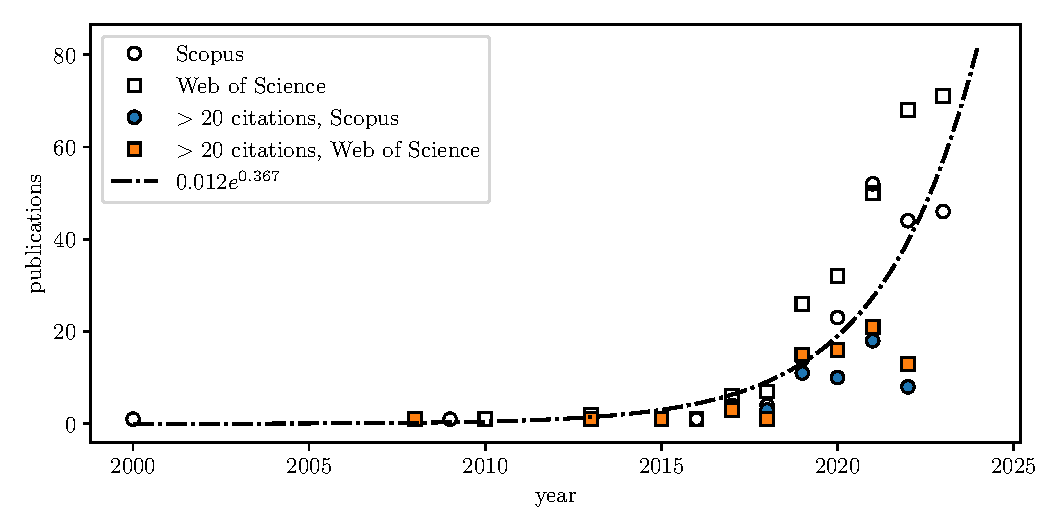
\includegraphics[width=\textwidth]{Figuras/bibliometric_review.pdf}
    \caption{Results of using the search query of Listing ref{lst:query} in \textit{Scopus} and \textit{Web of Science}. This figure displays how new this field of study is, and it also reveals an exponential rise in publications each year, both in terms of raw data and also when considering the more notable publications (those with more than 20 citations).}
    \label{fig:bibliometric_review}
\end{figure}

\citet{Bright2013} introduced a compressive sensing machine learning strategy for fluid dynamics, demonstrating efficient characterization of flow around a cylinder using sparse pressure measurements. This work paved the way for data-driven strategies in fluid mechanics, highlighting the potential of combining dimensionality reduction and convex optimization for flow field reconstructions. 

\citet{Zhang2015} advanced the field by examining machine learning models for data-driven turbulence modeling, focusing on reconstructing functions from high-fidelity simulation data. Their work addresses the importance of selecting appropriate learning algorithms and identified factors influencing model output, suggesting the strong potential of ML in augmenting traditional turbulence modeling approaches.

\cite{Wan2017a} introduced a reduced-space Gaussian Process Regression (GPR) for data-driven probabilistic forecasts of chaotic dynamical systems. By incorporating local interpolation error and phase space truncation uncertainties, they offered a novel perspective on forecasting complex systems, showing of the broader applicability of machine learning in uncertainty quantification and prediction within fluid dynamics.

In another work, \citet{Wang2017a} utilized detached eddy simulation (DES) and proper orthogonal decomposition (POD) to investigate unsteady flow behavior in steam turbine control valves. Their approach effectively demonstrated the synergy between simulation techniques and data-driven methods in understanding complex flow behaviors and their impact on valve performance.

The progression toward using evolutionary algorithms for the development of algebraic stress models, as explored by \citet{Weatheritt2017c}, further illustrates how machine learning methods can optimize fluid dynamics modeling beyond conventional approaches. This method offers a framework for creating tangible mathematical expressions of fluid dynamics phenomena, enhancing both accuracy and interpretability of turbulence models.

\citet{Bolton2019b} explored the use of convolutional neural networks for ocean data inference and subgrid parameterization. Their work demonstrated the capacity of deep learning models to replicate and predict subgrid-scale dynamics in oceanographic studies, marking a significant step forward in the use of ML for environmental fluid mechanics.

\citet{Demo2019c} combined POD with the active subspace property to enhance reduced order models (ROMs) for fluid dynamics. This innovative approach not only improved the accuracy of ROMs but also significantly reduced the computational cost of simulations .

Looking into fire safety, \cite{Hodges2019c} applied transpose convolutional neural networks for predicting compartment fire behaviors, showcasing how deep learning can offer rapid and robust predictions essential for safety assessments.

\cite{Jayaraman2019a, Zhu2019} delved into sparse reconstruction of fluid flows, demonstrating how learning from high-dimensional data can address challenges in aerodynamics and turbulence modeling. These contributions highlight the evolving landscape of fluid dynamics research, where data-driven methods are increasingly critical for advancing our understanding and capabilities in analyzing, predicting, and controlling fluid flows.

Complementing this, \citet{Geneva2020c} introduced a multi-fidelity deep learning model for surrogate modeling of turbulent flows. Their model, employing conditional invertible neural networks, marked a significant advance in capturing the complex dynamics of high Reynolds number flows, including turbulent wake behind bluff bodies. Such multi-fidelity approaches exhibit immense potential in providing accurate, yet computationally efficient, predictions of turbulent fluid flows.

On the search for efficient methodologies in data-driven predictions,\citet{Erichson2020b} presented a novel approach utilizing shallow neural networks for the reconstruction of fluid flow fields with limited sensors. Their methodology surpassed traditional modal approximation techniques in fluid mechanics, illustrating the effectiveness of neural networks in achieving high-quality flow field estimations from sparse datasets.

Another interesting application of ML is the reconstruction of velocity fields from experimental images, \cite{Barwey2022c}. They utilized CNNs to morph time-resolved experimental OH-PLIF images into corresponding three-component planar PIV fields, highlighting the powerful capability of CNNs in decoding complex fluid dynamics from experimental data, and to fill the gap between different types of experimental data, enhancing interpretability and utility.

The fast prediction of flow fields around airfoils using DL was tackled by \citet{Sekar2019}. By combining CNN and Multilayer Perceptron networks, they have demonstrated deep learning could offer fast and accurate flow field predictions, cutting down the time needed by traditional Navier-Stokes numerical solvers. This study highlighted the scalability and efficiency of using deep learning for aerodynamics research.

In a review that follows the above developments, \citet{Zhu2022a} provided an analysis of ML applications in multiphase flows and reactors. They enphasized the potential of ML in developing closure models, optimizing reaction conditions, and enhancing our understanding of complex flow and reaction mechanisms.

Further, the integration of Generative Adversarial Networks (GANs) in flow field prediction has received considerable attention. For instance, \citet{WU2022a} presented a data augmented GAN (daGAN) for efficient and accurate prediction of flow fields around airfoils, even with sparse training data. This work emphasizes the potential of GANs in augmenting existing datasets and enhancing the accuracy of prediction models, fostering advancements in aerodynamics and related fields.

\citet{Peters2023} presented an initial investigation into the application of a data-driven surrogate modeling technique, emphasizing rotor design applications. Their work demonstrated the capability of a proper orthogonal decomposition (POD)-based reduced-order model (ROM) derived from computational fluid dynamics (CFD) data for predicting rotor distributed loads across varying conditions with significantly reduced computational costs. On a related work, \citet{Lee2024} introduces an improved parametric model order reduction approach, particularly tailored for fluid-structure interaction analysis. Their methodology, a nonintrusive parametric model order reduction approach which combines POD with machine learning, demonstrated good performance on benchmark problems like the two-dimensional airfoil, showing of the potential in integrating machine learning with traditional model reduction techniques for fluid-structure interaction analysis.

In the realm of turbulence modeling, \citet{Li2024} illustrates the effectiveness of diffusion models (DMs) in reconstructing turbulent flow dynamics, showing superiority over classical generative adversarial networks (GANs) in both point-wise reconstruction and the statistical properties of inferred fields. \citet{Fujio2023} further explores Gaussian process latent variable modeling in conjunction with deep learning for robust predictions of scramjet flowfields, their ROM-based predictions showed the potential of the use of data-driven techniques for fast and accurate aerospace simulations.

In a similar way, \citet{Li2023a} developed a machine learning framework for modeling turbulent mixing flows within mechanically agitated vessels. Their approach, made use of supervised learning algorithms, show the potential of minimal data requirements to predict complex flow dynamics accurately, this could inspire further exploration into data-driven frameworks for multiphase flow systems. Additionally, \cite{Jin2024} introduced an extended dynamic mode decomposition framework integrated with an invertible dictionary learning, the method achieved enhanced performance in capturing the essential dynamics of data-driven systems. This work exemplifies the progress being made towards refining data-driven methodologies for better capturing physical systems' dynamics.

The exploration of indoor airflow fields through operator neural networks \cite{Gao2024}, represents a significant advance toward the fast prediction and efficient environmental control within building environments. Innovative computational strategies is further exemplified in \citet{Min2024}, where data-driven surrogate models where used in predicting the pressure fields around parallel twin cylinders, paving the way for computational savings in fluid dynamics (CFD) simulations.

Furthermore, the correction of coarse grid CFD simulations using machine learning post-processing tools as detailed by \citet{Kiener2023} lead to promising in blending data-driven methodologies with traditional simulation techniques to achieve greater accuracy in aerodynamic analysis. The time-variant prediction of flow over an airfoil using deep neural network models, as proposed by \cite{Peng2020b}, alongside the research by \citet{Reinbold2021d} on learning models from noisy and incomplete experimental data, show the transformative impact of machine learning in modeling complex physical phenomena from experimental observations.

Similarly, the employment of supervised learning for physical field reconstruction \cite{Liu2021c}, and the novel method of analyzing unsteady flow fields using deep autoencoders in \cite{Omata2019c}, illustrate the expanding frontiers of data-driven methods in capturing the intricacies of fluid dynamics. \citet{Liu2021c} introduced a method using deep convolutional neural networks (CNNs) to predict physical fields in a heat transfer problem, showcasing the effectiveness of data-driven approaches in capturing complex flow behaviors. Similarly, \citet{Riel2021c} developed a PINN framework to infer variations in drag across glacier beds, demonstrating the versatility of PINNs in geophysical flow applications. These studies underscore the adaptability of PINNs in accurately modeling fluid dynamics across diverse domains.

The work on neural network-based eddy-viscosity correction for RANS simulations by \cite{Volpiani2022}, and the challenges in fast flow field prediction of hydrofoils tackled through deep learning by \cite{Li2023}, offer valuable insights into the integration of computational techniques with machine learning for enhanced fluid dynamics modeling.

The afforementioned recent studies represent only a fraction of ongoing efforts to merge data-driven methodologies with fluid dynamics, promising to revolutionize predictions and control in fields like aerospace and environmental sciences. The literature review highlights a dynamic new era where machine learning (ML) and deep learning (DL) are increasingly applied, offering fresh insights, faster simulations, and enhanced predictive capabilities for complex flow phenomena. This integration of data-driven approaches with traditional fluid dynamics marks a revoltion, driving advancements in simulation efficiency. This body of work illuminates current trends and methodologies and also sets the stage for further exploration and discourse in the field.


\section{Bibliographic Review in Nozzle Flow}

\section{Conclusion}
%%% =============================
%%      IMPORTANTE
%% ESTE ARQUIVO DEVE ESTAR SALVO COMO
%%      UTF - 8
%% =============================

% ----------------------------------------------------------
% Este capítulo é parte integrante do arquivo mestre
% Relatorio_TCC_Mestrado_Base_VERSÃO_SUBVERSÃO_FHZ
% ----------------------------------------------------------


% ----------------------------------------------------------
\chapter{Methodology}
\label{chap:methodology}
% ----------------------------------------------------------
The flow reconstruction methodology concerns aligning intricate simulations with less detailed counterparts in a practical manner, enabling the recreation of detailed flow patterns based on simplified simulations. This process comprises two primary stages: the dimensionality reduction step and the regression step.

The aim of the dimensionality reduction step is to facilitate the subsequent regression process by substantially reducing the number of variables employed as both input and output.
aleviating the known and up to date \textit{curse of dimensionality} problem.

In the context of the regression step, various function approximators can be employed. Neural Networks are a favorable choice due to their longstanding presence in the field of machine learning and their capability to handle extensive datasets from simulations, even when confronted with a plethora of variables (constituting our inputs and outputs). Alternatively, Gaussian processes, particularly in the form of Kriging, present themselves as a viable option owing to their expedited computational efficiency and interpretability, facilitated by their closed-form formulation.

The present flow reconstrudtion methodology is a purely data-driven approach and should work seamsly with either experimental or numerical data. For the sake of reducing costs and time requirements, this work is limited to the data syntheticly generated using numerical solvers. The follwing sections will describe the steps involved in the data generation, pre-processing, and post-processing of the flow fields in order to obtain the reduced order surregate surrogate model.

The main objective of the flow reconstruction strategy is to build a surrogate model able of predicting high-fidelity flow fields by using low fidelity data. The low fidelity data can be either sparse measurments of experimental data or numerical data generated by using fast and inaccurate solvers, generally, this low fidelity solver disregard some dimensions, physics involved, or both.

% Numerical solvers often returns large filds with a huge number of deegre of freedom. This could be a problem for the training process of the surrogate models, this problem first described by  as the \textit{curse of dimensionality}.

% This surrogate model is data-driven and trained using a dataset of low- and high-fidelity simulations. As the number of features to be modeled can be high, we employ a dimensionality reduction strategy using Singular Value Decomposition (SVD) to compress the datasets of low- and high-fidelity simulations. The functional mapping between these two distinct spaces is performed using a regression strategy such as Kriging or Neural Networks.

% The flow reconstruction methodology concerns aligning intricate simulations with less detailed counterparts in a practical manner, enabling the recreation of detailed flow patterns based on simplified simulations. This process comprises two primary stages: the dimensionality reduction step and the regression step.

% The aim of the dimensionality reduction step is to facilitate the subsequent regression process by substantially reducing the number of variables employed as both input and output.

% In the context of the regression step, various function approximators can be employed. Neural Networks are a favorable choice due to their longstanding presence in the field of machine learning and their capability to handle extensive datasets from simulations, even when confronted with a plethora of variables (constituting our inputs and outputs). Alternatively, Gaussian processes, particularly in the form of Kriging, present themselves as a viable option owing to their expedited computational efficiency and interpretability, facilitated by their closed-form formulation.

\section{Data Driver Approach}

Since our method relies entirely on data, where the data comes from doesn't really mattet, it could be gathered through experiments or artificially created using any numerical method. In this study, we're using synthetic data because it makes it easier, quickier, and cheapier to control numerical experiments, especially it allow us to generate dataset with different sizes and also evalueate our methodoloty with respect to data availability.

Regardless of the situation, the first step is to gather two sets of data: one representing the low fidelity space, it is our input, denoted by $\mathbf{X}$ and the other represent the targed high fidelity data, denoted by $\mathbf{y}$. The low-fidelity data could be a simulation with a rough grid, shortened dimensions, or other simplifications, and it might only include global scalar variables like geometry parameters and averaged boundary conditions. In constrast, the high-fidelity dataset usually involves the results of multidimensional simulation, able to capture as much of the physics as possible.

\section{Defining Data Matrix}

\section{Dimensionality Reduction}

\subsection{Numerical/Aplied Linear Algebra}

Linaer algera can simply be estated as the mathematics of vector and matrix, as so it has a paramout importance in many fields, including machine learning.

Numerial Linear algebra study how to aply linear algera to perform fast and accurate calculations using computers. This to objectives encouter two main complications, machine precision and machine speed.

Multidimensional vectors can be used to represet a lot of different complicated things, like images, mearusrements, voice, data, text and so forth.

Matrix is a grid o number or a list of vectors.

The flow reconstruction technique is specifically devised for addressing fluid flow fields, where the number of degrees of freedom is intricately tied to the elements in a full-order numerical simulation. In 3D flow fields, this association can result in an exceedingly large number of degrees of freedom, often reaching millions or even billions. Even in the context of the simplified 2D numerical simulation presented in this study, the number of degrees of freedom is on the order of $10^4$. This numerical value signifies the variables that the surrogate model must encapsulate. Therefore, any reduction in this count not only reflects a judicious application of compressed data but also yields a more cost-effective model.

In addition to the computational efficiency gained by diminishing the computational burden required for modeling the flow field, the process of dimensionality reduction also enhances the model's fitting capabilities. This is owing to the substantial reduction in the number of coupled linear equations that need to be modeled. In essence, the streamlined approach not only contributes to computational economy but also augments the model's efficacy in representing the underlying fluid dynamics.

To enact data compression, the matrices that compile training snapshots for low-fidelity and high-fidelity simulations, denoted as $\mathbf{X}_{l}$ and $\mathbf{X}_h$ respectively, underwent compression utilizing the truncated Singular Value Decomposition (SVD) technique. In essence, the SVD factorization, expressed in equation \ref{eq:svd}, possesses the capability to precisely represent any matrix $\mathbf{X}$ if the number of elements in the diagonal of the square singular values matrix $\mathbf{\Sigma}$ equals the original rank of the matrix $\mathbf{X}$. 

\begin{equation}
    \mathbf{X} = \mathbf{U}\mathbf{\Sigma}\mathbf{V}^T   
\end{equation}

Data compression is then achieved by truncating the number of singular values, retaining only the most significant ones, those with higher absolute values arranged in decreasing order. This process serves to distill essential information from the matrices, offering an effective means of compression while maintaining fidelity to the underlying data structure.

\subsection{Truncated SVD}

The singular value decomposition (SVD) is one of the most relevant and widelty used matrix factorization algorithm in numerical linear algebria, with many application such as dimensionality reduction and approximate solution for linear system of equations. In the context of this work the SVD will be used to perform a low-rank approximation of a generic data matrix $\mathbf{X}$ containing $m$ samples with dimensiolaity $n$. Given a generic data matrix $\mathbf{X}$, with row dimension $m$ representing the samples count and the column dimension $n$ representing the dimension or degree of freedom of each sample, the inner dimension $r$, or  matrix \textit{rank},  If $\mathbf{X}$ is at full rank, its decomposition into $\mathbf{X}$ and $\mathbf{B}$ provides a unique solution to the equation.

\begin{equation}
    \mathbf{X}_{m \times n} = \mathbf{B}_{m \times r} \times \mathbf{C}_{r \times n}.
\end{equation}

In fact the matrix $\mathbf{X}$ can be stored efficiently if whe are able to find a low rank approximation, such that $k << r$. In this case storing both $\mathbf{B}$ and $\mathbf{C}$ requires $(m+n)k$ storage units, instead of $mn$ for the full rank $\mathbf{X}$. Analougously, a matrix-vector multiplication would require $(m+n)k$ operations insteady of $mn$. The factorization also reveals relevat properties of the data in matrix $\mathbf{X}$.

\begin{equation}
    \mathbf{X}_{m \times n} \approx \mathbf{B}_{m \times k} \times \mathbf{C}_{k \times n}.
\end{equation}

This approximatio is extremely usefful to tackle the \textit{curse of dimensionality} problem. The low-rank approximation can be obtained by factoring the matrix $\mathbf{X}$ into orthonormal left $\mathbf{U}$ and right $\mathbf{V}^\dagger$ singular vectors and an $r$-dimensional non-negative diagonal matrix $\mathbf{\Sigma}$, of singular values ordered in descending order.

\begin{equation}
    \mathbf{X}_{m \times n} = \mathbf{U}_{m \times k} \mathbf{\Sigma}_{k \times k} {\mathbf{V}^\dagger}_{k \times n}
\end{equation}

This task can be performed by forming a small matrix $\mathbf{B}$, such that

\begin{equation}
    \mathbf{B}_{m \times k} = \mathbf{Q}_{m \times k}^\dagger \mathbf{X}_{k \times k} 
\end{equation}

And the computing the singular value decomposition of $\mathbf{B}$

\begin{equation}
    \mathbf{B}_{m \times k} =  \mathbf{\tilde U}_{m \times k}^\dagger \mathbf{\Sigma}_{k \times k} \mathbf{V}_{k \times k}^\dagger
\end{equation}

Finally projecting 

\begin{equation}
    \mathbf{U}_{m \times n} = \mathbf{Q}_{m \times k}\mathbf{U}_{k \times k}
\end{equation}

The matrix $\mathbf{Q}$ is the orthonormal matrix that forms a basis for the range of $\mathbf{X}$, it can be efficiently computed using randomized algorithms to solve the problem of given $k < min(m,n)$, finding a $m \times k$ matrix such that

\begin{equation}
    \mathbf{X} \approx \mathbf{Q} \mathbf{Q}^\dagger \mathbf{X}
\end{equation}

Matrix $\mathbf{Q}$ can be computed directly by a QR factorization in the form of $\mathbf{X} \approx \mathbf{Q}\mathbf{R}\mathbf{P}$ and then setting $\mathbf{B} = \mathbf{P}^\dagger \mathbf{R}$. Instead, to solve it using a randomized sampling we start by building random matrix $\mathbf{\Omega}_{n \times k}$, suppose it to be Gaussian. Then pré-multiply it

\begin{equation}
    \mathbf{Y} = \mathbf{X} \mathbf{\Omega}
\end{equation}

Construct a orthonormal matrix $\mathbf{Q}$ such that

\begin{equation}
    \mathbf{Y} = \mathbf{Q} \mathbf{Q}^dagger \mathbf{X}
\end{equation}

the basis vector $\mathbf{Q}$ and its self adjoint or conjugate transpose matrix $\mathbf{Q}^{\dagger}$, satisfying

\begin{equation}
    \mathbf{X} \approx \mathbf{Q}^{\dagger} \mathbf{Q} \mathbf{X}
\end{equation}

A randomized algorithm is used to find $\mathbf{Q}$ tha minimizaes

\begin{equation}
    \norm{\mathbf{X} - \mathbf{Q}^{\dagger} \mathbf{Q} \mathbf{X}} 
\end{equation}

\begin{equation}
    \mathbf{B} = \mathbf{Q}^{\dagger} \times \mathbf{X}
\end{equation}

Continue to compile due to autosave. New entry. 

\section{POD}

POD, also known as principal component analysis (PCA), empirical orthogonal functions (EOF), the Hotelling transform, or a Karhunen-Loeve expansion in various domains, is a technique to reduce the dimensionality of complex data sets. This method is extensively used in numerical simulations and physical experiments to extract dominant patterns of variability from a high-dimensional dataset.

%%% Local Variables:
%%% mode: LaTeX
%%% TeX-master: "../thesis_allan"
%%% End:

%\chapter{Transonic Nozzle Flow Reconstruction}
\label{chap:Case_Study}

To evaluate the performance of the method, a case study was selected for the reconstruction of supersonic flow of hot air inside a nozzle. The availability of experimental data and a comprehensive apparatus description \citep{Back1965a} provided us with the necessary resources to validate the numerical methods used to generate training and test datasets. This case study also poses a challenging scenario for the surrogate model, involving the reconstruction of flow fields with discontinuous shock wave structures.

In this case study we perform a dimensiolaity reduction study to investigate the impact of the reduced basis dimension on the overall reconstruction strategy, the model accuracy was also evaluate in function of three diffent data set sizes and also with respect to the construction of the entry quantities in the low fidelity data matrix $\mathbf{x}$. We also performed neural network hyperparameter optimization and compared the results agains the Gaussian process method.

\section{The Nozzle Geometry}

The fluid behavior inside the nozzle is largely dependent not only on thermodynamic boundary conditions on its entrance and exits, but also on the geometric configuration of the walls. To made the surrogate model sentive to the geometric configuration the nozzle was constructed in parametrically in a CAD software (opensource FreeCAD), following the parameters of the $45^\circ-15^\circ$ nozzle described in \cite{Back1965a} and listed in Table \ref{tab:geom_params}.

\begin{table}[h]
    \centering
        \begin{tabular}{ r l r l }
            \hline
            \textbf{description}               & \textbf{parameter} & \textbf{value} & \textbf{units} \\ 
            \hline
            \hline
            \symbl{$L_i$}{Distante to $r_i$ center}
            {Distante to $r_i$ center}           & $L_{i}$         & 7.874   & mm \\
            \symbl{$L_{tht1}$}{Convergent $r_c$ tangency distance}
            {Convergent $r_c$ tangency distance} & $L_{tht1}$      & 55.880  & mm \\
            \symbl{$L_{tht2}$}{Divergent $r_c$ tangency distance}
            {Divergent $r_c$ tangency distance}  & $L_{tht2}$      & 68.148  & mm \\
            \symbl{$L_{th}$}{Length to throat}
            {Length to throat}                   & $L_{th}$        & 64.872  & mm \\
            \symbl{$L_{ti}$}{Length to $r_i$ tangency}
            {Length to $r_i$ tangency}           & $L_{ti}$        & 22.250  & mm \\
            \symbl{$L_{to}$}{Length to $r_o$ tangency}
            {Full length}                        & $L$             & 185.039 & mm \\
            \symbl{$r_{c}$}{Curvature radius at contraction}
            {Curvature radius at contraction}    & $r_{c}$         & 12.700  & mm \\
            \symbl{$r_{i}$}{Curvature radius at inlet}
            {Curvature radius at inlet}          & $r_{i}$         & 20.320  & mm \\
            \symbl{$r_{in}$}{Inlet radius}
            {Inlet radius}                       & $r_{in}$        & 63.500  & mm \\
            \symbl{$r_{th}$}{Throat radius}
            {Throat radius}                      & $r_{th}$        & 20.320  & mm \\
            \symbl{$r_{out}$}{Outlet radius}
            {Outlet radius}                      & $r_{out}$       & 63.298  & mm \\
            \symbl{$\theta_{div}$}{Divergence angle}
            {Divegence angle}                    & $\theta_{div}$  & 15.000  & deg \\
            \symbl{$\theta_{conv}$}{Convergence angle}
            {Convergence angle}                  & $\theta_{conv}$ & 45.000  & deg \\
            \hline
        \end{tabular}
    \caption{Geometric parameters and values for baseline model of reference \cite{Back1965a}.}
    \label{tab:geom_params}
\end{table}

The parameters in Table \ref{tab:geom_params} specifies a conical nozzle with a $\theta_{conv}$ angle of convergence,  $\theta_{div}^\circ$ angle of divergence, and a fixed circular inlet radius $r_{in}$. The overval nozzle lenght $L_{th}$ and throat nozzle lenght $L_{th}$ is also fixed. Due to axisymmetry, only the specification of the upper contour is sufficient to construd a parametric CAD model as show in Figure \ref{fig:geom_params}.

\begin{figure}[h]
    \centering
        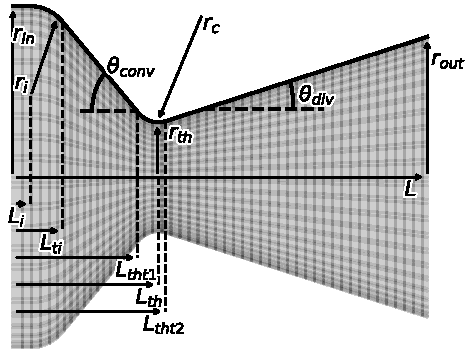
\includegraphics[width=0.50\linewidth]{Figuras/geometry_figures/nozzle_15_xy.pdf}
        \caption{Parametrized nozzle geometry.}
        \label{fig:geom_params}
\end{figure}

The geometry variability is obtained by varying the divergence angle $\theta_{div}$ and as a consequence the outlet radius $r_{out}$ while kepting the all remaining geometric paremeters constant. Such modification alter the area ratio after the troat as show in Figures \ref{fig:nozzle_10}, \ref{fig:nozzle_15} and \ref{fig:nozzle_20}, and is sufficient to impact the flow acceleration or deceleration, after the throat, determining if a shock is likely to form, and if it is the case the position of normal shock and structure of oblique shocks.

\begin{figure}[t]
    \centering
    \begin{subfigure}{0.3\textwidth}
        \centering
        % include second image
        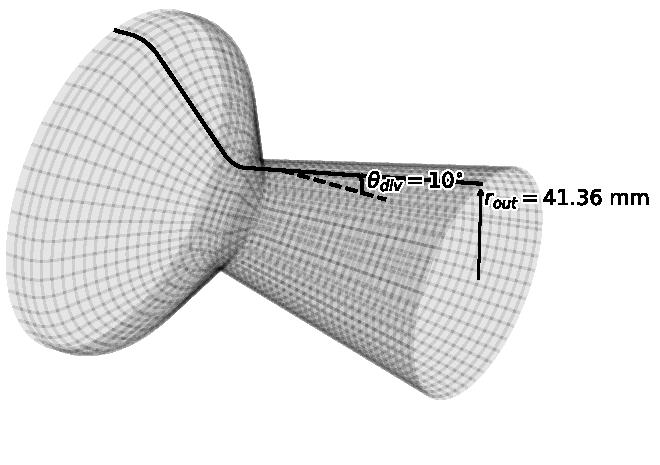
\includegraphics[width=\linewidth]{Figuras/geometry_figures/nozzle_10.pdf}  
        \caption{$\theta_{div}=10^{\circ}$.\label{fig:nozzle_10}}
    \end{subfigure}
    \begin{subfigure}{0.3\textwidth}
        \centering
        % include second image
        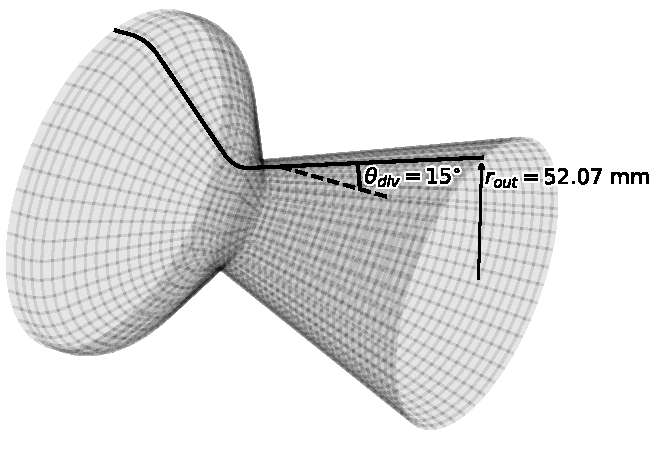
\includegraphics[width=\linewidth]{Figuras/geometry_figures/nozzle_15.pdf}  
        \caption{$\theta_{div}=15^{\circ}$.\label{fig:nozzle_15}}
    \end{subfigure}
    \begin{subfigure}{0.3\textwidth}
        \centering
        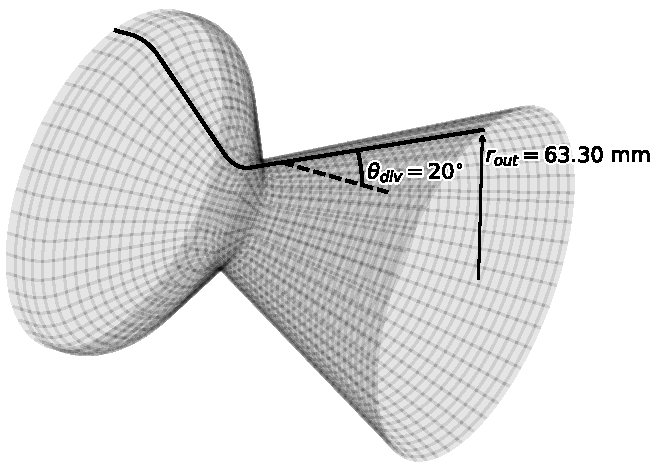
\includegraphics[width=\linewidth]{Figuras/geometry_figures/nozzle_20.pdf}  
        \caption{$\theta_{div}=20^{\circ}$.\label{fig:nozzle_20}}
    \end{subfigure}
    \caption{Parametrized Nozzle geometries, (b) is the baseline.}
\end{figure}

The CAD model is encapsulated into an abstract class, from withinh the nozzle area variation is conputed to be input in thw low fidelity cfd model and also a numerical domain is build for the high fidelity model.

\section{Numerical Methods}

The \textit{low fidelity} solutions  were obtained using a finite volume solver for the steady-state Euler equations, with a detailed description provided in Section \ref{sec:q1d_euler}. This method saves computing time by assuming the flow to be non-viscous and the domain to be one-dimensional, with only the cross-sectional area of the nozzle allowed to vary along the symmetry axis.

For the \textit{high fidelity} solutions, the steady-state compressible Reynolds-Averaged Navier-Stokes equations were solved using the open-source finite volume solver SU2, with details of the implementation provided in Section \ref{sec:2d_navier_stokes_solver}. Due to intrinsic axisymmetry, the domain was assumed to be two-dimensional. This method is able to model turbulence effects using the shear stress transport closure, and also, boundary conditions other than adiabatic could be used on the nozzle walls.

\subsection{Quasi-1D Euler Solver}
\label{sec:q1d_euler}

The hot flowing air inside the nozzle is considered to be a compressible and calorically perfect gas. The set of equations for conservation of mass, momentum, and energy forms the well-known quasi-1D Euler equations, written compactly in vector notation as Equation \eqref{eq:q1d_euler_vec}.

\begin{equation}
    \symbl{$\partial$}{Partial derivative}
    \frac{\partial}{\partial t}{\mathbf{U}}  + \frac{\partial }{\partial x}\mathbf{F} = \mathbf{S} 
    \label{eq:q1d_euler_vec}
\end{equation}

Denoting the primitive variables specific mass as $\rho$, x-component velocity as $u$, pressure as $p$, and the specific total energy as $e$, and with the cross-sectional area denoted as $A$, these vectors are formed as shown in Equation \eqref{eq:q1d_euler_vectors}.

\begin{eqnarray}
    \symbl{$\partial$}{Partial derivative}
    \mathbf{U} = \begin{bmatrix} \rho \\ \rho u \\ e \end{bmatrix} & \mathbf{F} = \begin{bmatrix} \rho u \\ \rho u^2 + p \\ (e+p)u \end{bmatrix} & \mathbf{S} = \begin{bmatrix} 0 \\ \frac{p}{A} \frac{dA}{dx} \\ 0 \end{bmatrix}
    \label{eq:q1d_euler_vectors}
\end{eqnarray}

A steady state numerical solution for this system of equations is found by usign a time marching numerical scheme, as in equation \eqref{eq:time_marching}

\begin{equation}
   \mathbf{U}^{n+1} = \mathbf{U}^{n} + \Delta t^n \mathbf{R} (\Delta t^n, U^n) 
   \label{eq:time_marching}
\end{equation}

, the residual, \eqref{eq:q1d_euler_res}, for each time step is computed using a finite volume method discretization over the 1D domain, represented graphically in Figure \ref{fig:1d_domain}.

\begin{figure}
\centering
\begin{tikzpicture}[scale=1.9]
	\draw [thick] (0,0) -- (6,0);
	\draw [dashed,thick] (-1,0) -- (0,0);
	\draw [->,dashed,thick] (6,0) -- (7,0);

	\node at (7.2,0) {$x$};

    \def\celllabel[#1](#2){
        \node[fill=black,circle, scale=0.0, label={[yshift=2mm]above:$#2$}] at (#1+0.5,0) {};
    }

    \def\cell(#1){
        \node[fill=black,circle, scale=0.5] at (#1+0.5,0) {};
    }

    \def\ghostcell(#1){
        \node[circle, draw=black, fill=white, scale=0.5] at (#1+0.5,0) {};
    }

    \def\face(#1){
        \draw (#1,0.1) -- (#1, -.1); 
    }

    \def\facelabel[#1](#2){
        \node[scale=0.0, label={[yshift=-2mm]below:$#2$}] at (#1,0) {};
    }

    % draw faces
	\foreach \i in {0,1,...,6}{
		\face(\i);	
	}

    % draw face labels
    \facelabel[3](i-1/2);
    \facelabel[4](i+1/2);

    % draw cell centers
    \foreach \i in {0,1,...,5}{
        \cell(\i);
	}

    % draw ghost cells
    \ghostcell(-1);
    \ghostcell(6);

    % draw cell labels
    \celllabel[-1](0);
    \celllabel[0](1);
    \celllabel[1]($\ldots$);
    \celllabel[2](i-1);
    \celllabel[3](i);
    \celllabel[4](i+1);
    \celllabel[5]($\ldots$);
    \celllabel[6](N);
\end{tikzpicture}
\label{fig:1d_domain}
\caption{Quasi one dimensional domain discretization for the cell-centered finite volume method.}
\end{figure}

\begin{equation}
\mathbf{R}(\Delta t^n, U^n) = \mathbf{S}_i^n - \frac{1}{\Delta x_i} \left( \mathbf{F}^{n}_{i+1/2} - \mathbf{F}^{n}_{i-1/2} \right) 
\label{eq:q1d_euler_res}
\end{equation}

The system of equations is then integrated in time using a 4th-order Runge-Kutta scheme, whit timestep $\Delta t$ determined by imposiv a CFL number

\begin{align}
    k_1 &= \mathbf{R}(t^n, U^n)  \\
    k_2 &= \mathbf{R}(t^n + \frac{\Delta t^n}{2}, U^n +  \Delta t^n \frac{k_1}{2}) \\
    k_3 &= \mathbf{R}(t^n + \frac{\Delta t^n}{2}, U^n +  \Delta t^n \frac{k_2}{2}) \\
    k_4 &= \mathbf{R}(t^n + \Delta t^n, U^n + \Delta t^n k_3) \\
    \mathbf{U}^{n+1} &= \mathbf{U}^n + \frac{1}{6}(k_1 + 2k_2 + 2k_3 + k_4)
\end{align}

The quasi one-dimensional numerical method used in this work is an in-house cfd solver for the compressible Euler equations \eqref{eq:q1d_euler_vec}. Altough the method can capture compressible effects and shock formation, the shock is sharper than the viscous one. The method is also unable to predict the diamond structure of oblique shocks. The method also does not take into account any prescribed tempeture in the wall. 

\subsubsection{Numerical Verification and Validation}

To evaluate the validity of the method, results from our implementation was compered with numerical results obtained by

NUMERICAL VALIDATAION/VERIFICATION

\subsection{2D Navier-Stokes Solver}
\label{sec:2d_navier_stokes_solver}

The compressible Navier-Stokes equation \eqref{eq:ns_equations} was solved in 2D.

\begin{equation}
    \mathbf{R(\mathbf{U})} = \frac{\partial \mathbf{U}}{\partial t} + \nabla \cdot \mathbf{F}^c(\mathbf{U}) - \nabla \cdot \mathbf{F}^v(\mathbf{U}, \nabla \mathbf{U}) - \mathbf{S}
    \label{eq:navier-stokes}
\end{equation}


\begin{eqnarray}
   %\symbl{$\partial$}{Partial derivative}
   \mathbf{U} = \begin{bmatrix} \rho \\ \rho \mathbf{v} \\ \rho E \end{bmatrix} 
   & \mathbf{F}^c = \begin{bmatrix} \rho \mathbf{v}  \\ \rho \mathbf{v}\otimes \mathbf{v} + \mathbf{1} p \\ \rho E \mathbf{v} + p \mathbf{v} \end{bmatrix} 
   & \mathbf{F}^v = \begin{bmatrix} \cdot \\ \boldsymbol{\tau} \\ \boldsymbol{\tau} \cdot \mathbf{v} + \kappa \nabla T \end{bmatrix} 
   %& \mathbf{S} = \begin{bmatrix} 0 \\ 0  \\ 0 \end{bmatrix}
   \label{eq:ns_equations}
\end{eqnarray}

, with a viscous stress tensor given by 

\begin{equation}
    \boldsymbol{\tau} = \mu \left( \nabla \mathbf{v} + \nabla \mathbf{v}^T \right) - \mu \frac{2}{3} \mathbf{1} \left( \nabla \cdot \mathbf{v} \right)
    \label{eq:ns_stress_tensor}
\end{equation}

The viscosity is

\begin{equation}
    \mu = \mu_d + \mu_t
    \label{eq:mu}
\end{equation}

and the thermal conductivity

\begin{equation}
    \kappa = \frac{\mu_d + c_p}{Pr_d} + \frac{\mu_t c_p}{Pr_t}
    \label{eq:kappa}
\end{equation}

where $\rho$ is the fluid density, $\mathbf{v} = \left\{ u , v \right\}^T \in \mathbb{R}$ is the flow velocity vector, with $u$ and $v$ being its components. $E$ is the total energy per unit mass, $p$ the static pressure, $\boldsymbol{\tau}$ the viscous stress tensor, $T$ the static temprature, $\kappa$ the thermal conductivity, and $\mu$ the viscosity.

With an assumption of a perfect gas, with constant specific heat ratios $\gamma$, and gas constant $R$, the system can be closed using the relation for pressure

\begin{equation}
    p = \rho \left( \gamma - 1 \right) \left[ E - \frac{1}{2} \left( \mathbf{v} \cdot \mathbf{v} \right) \right]
    \label{eq:pressure}
\end{equation}

The SU2 software \cite{Economon2016a} was employed, the Reynolds Averaged Navier-Stokes equations were solved using the finite volume method and the SST (Shear Stress Transport) turbulence model. To obtain the steady-state solution, the implicit Euler integration method was utilized in conjunction with time marching.

\subsubsection{Grid Independence Study}

A Grid Independence Study using the Grid Convergence Index (GCI) \cite{Roache1994} was performed to assess numerical accuracy. Table 1 lists the three mesh levels used and Table 2 shows the results. Positive p and small GCI values indicate a monotonic and asymptotic convergence, respectively. A GCIasymptotic close to 1 indicates grid-independent solutions, so Medium was chosen for further analysis (shown in Figure 2).

\begin{table}
\centering
\begin{tabular}{lccccccc}
\toprule
        & $ \bar{p} $ & $ N_{cells} $ & $ r $ & $ GCI $ & $ \bar{p}_{extrapolated} $ & $ order $ &  $ GCI_{asymp.} $ \\ \midrule
Fine    & $9.995\times10^4$ & $6000$  & $1.5$ & $0.17$ \% &  \multirow{3}{*}{$1.00\times10^5$} &  \multirow{3}{*}{$1.99$} &  \multirow{3}{*}{$1.002$} \\ 
Medium  & $9.980\times10^4$ & $2500$  & $1.3$ & $0.41$ \% & & & \\ 
Coarse  & $9.950\times10^4$ & $1500$  & -     & -         & & & \\ 
        & $ \bar{T} $ & $ N_{cells} $ & $ r $ & $ GCI $ & $ \bar{T}_{extrapolated} $ & $ order $ &  $ GCI_{asymp.}$ \\ \midrule 
Fine    & $6.909\times10^2$ & $6000$  & $1.5$ & $0.00$ \% &  \multirow{3}{*}{$6.91\times10^2$}  &   \multirow{3}{*}{$8.14$} &   \multirow{3}{*}{$1.000$} \\ 
Medium  & $6.910\times10^2$ & $2500$  & $1.3$ & $0.04$ \% & & & \\ 
Coarse  & $6.930\times10^2$ & $1500$  & -     & -         & & & \\ 
\bottomrule
\end{tabular}
\caption{Grid convergence study over 3 grids.}
\label{tab:gci_study}
\end{table}

\begin{figure}[h]
  \centering
  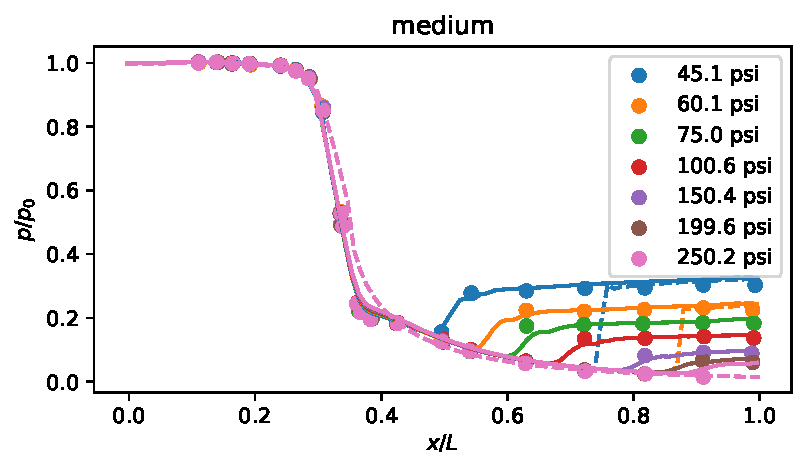
\includegraphics[width=\linewidth]{Figuras/validation/validation_medium.pdf}
  \caption{Validation using all experimental data of reference \cite{Back1965a} for the nozzle in question.}
  \label{fig:validation_su2}
\end{figure}

\section{Design of Eperiments}

As the method is data driven, data must be gattered or generated. In this study three distincts datasets was generated using a Latin Hypercube Sampling using 1000 iterations to maximize the minimal \textit{pdist}. The ranges for the independent variables is described in Table \ref{tab:doe_lhs}. The surrogate model should be able to reconstruct any flow field of simulations within the precribed design of experiment space of parameters. The dataset consist onluy of converged simulations, the convergence criteria utilized is the maximum residue of $10^{-8}$ for the mass, momementum and energy equation. The dataset was also split into training, validation and test, using $90$ \% of total data for training, 5 \% for validation and the remaining 5 \% for testing.

\begin{table}[h!]
  \centering
  \begin{tabular}{lrlcccc} 
   \toprule
   \multirow[b]{3}{*}{\makecell[l]{Wall \\ Boundary \\ Condition}} & \multirow[b]{3}{*}{\makecell[r]{Dataset \\ Size}} &  \multirow[b]{3}{*}{\makecell[l]{\makecell[l]{(Training, \\Validation, \\Test)} }} & \multicolumn{4}{c}{Independent Parameters} \\
    &  & & $p_0$ [MPa] & $T_0$ [K] & $\theta_{div}$ [$^\circ$] & $T_w$ [K]\\
    &  &  & \makecell{(min,\\max)} & \makecell{(min,\\max)} & \makecell{(min,\\max)} & \makecell{(min,\\max)} \\
   \midrule
   \multirow{3}{*}{\makecell[l]{Prescribed \\ Temperature}} & Small & $(130,17,16)$ & \multirow{3}{*}{\makecell{$(0.35$,\\$1.70)$}} & \multirow{3}{*}{\makecell{$(300.00,$\\$ 800.00)$}} & \multirow{3}{*}{\makecell{$(10.00$,\\$20.00)$}} & \multirow{3}{*}{\makecell{$(120.00$,\\$300.00)$}} \\ 
   & Medium & $(332,42,41)$ &  &  & & \\
   & Large & $(652,82,82)$ &  &  & & \\
   \midrule
   \multirow{3}{*}{Adiabatic} & Small & $(128,17,16)$ & \multirow{3}{*}{\makecell{$(0.35$,\\$1.70)$}} & \multirow{3}{*}{\makecell{$(300.00,$\\$ 800.00)$}} & \multirow{3}{*}{\makecell{$(10.00$,\\$20.00)$}} &  \\ 
   & Medium & $(323,41,40)$ &  &  & & \\
   & Large & $(644,81,81)$ &  &  & & \\ 
   \bottomrule
  \end{tabular}
  \caption{Dataset ranges for design variables and final dataset sizes retaining converged simlation.}
  \label{tab:doe_lhs}
\end{table}

Since our method relies entirely on data, where the data comes from doesn't matter—it could be gathered through experiments or artificially created using any numerical method. In this study, we're using synthetic data because it makes it easy and quick to control numerical experiments, especially in terms of the number of experiments and the quality of the data.

Regardless of the situation, the first step is to gather two sets of data: one with low fidelity and the other with high fidelity. The low-fidelity data could be a simulation with a rough grid, shortened dimensions, or other simplifications, and it might only include global scalar variables like geometry parameters and averaged boundary conditions. In the world of fluid dynamics, the high-fidelity dataset usually involves multidimensional simulations, trying to capture as much of the physics as possible.

\begin{figure}[t]
    \centering
    \begin{subfigure}{0.3\textwidth}
        \centering
        % include second image
        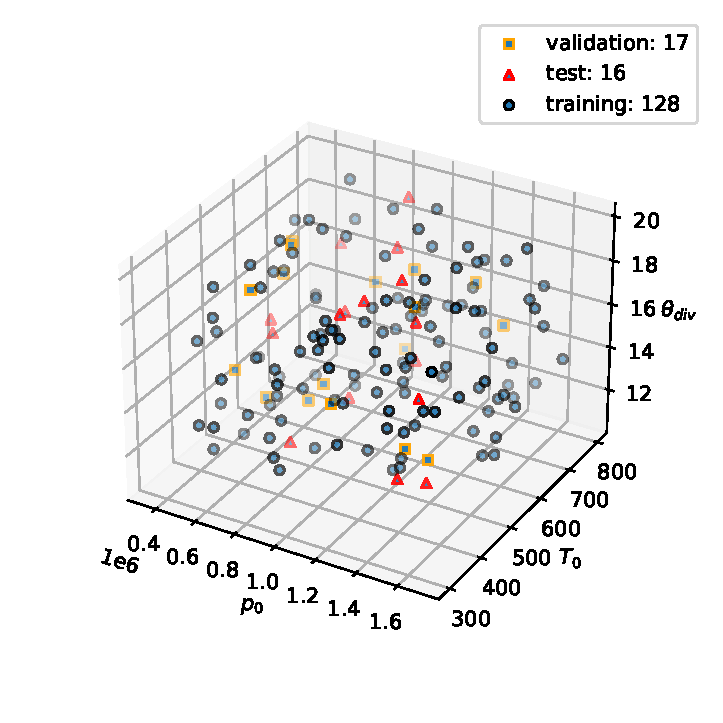
\includegraphics[width=\linewidth]{Figuras/lhs/data_adiabatic/doe_200/lhs_all.pdf}  
        \caption{Small dataset.}
        \label{fig:lhs_adiabatic_200}
    \end{subfigure}
    \begin{subfigure}{0.3\textwidth}
        \centering
        % include second image
        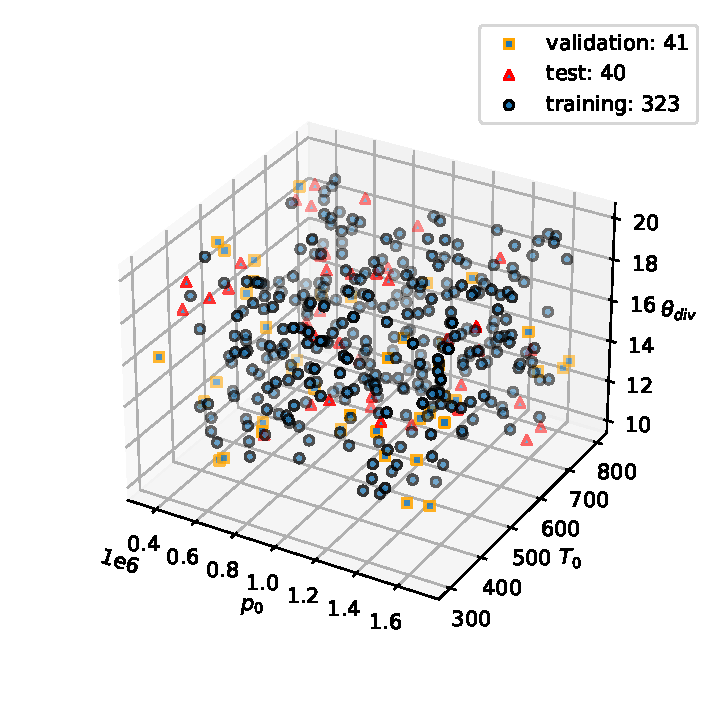
\includegraphics[width=\linewidth]{Figuras/lhs/data_adiabatic/doe_500/lhs_all.pdf}  
        \caption{Medium dataset.}
        \label{fig:lhs_adiabatic_500}
    \end{subfigure}
    \begin{subfigure}{0.3\textwidth}
        \centering
        \includegraphics[width=\linewidth]{Figuras/lhs/data_adiabatic/doe_1000/lhs_all.pdf}  
        \caption{Large dataset.}
        \label{fig:lhs_adiabatic_1000}
    \end{subfigure}
    \caption{Latin Hypercube Sampling for Design of Experiments with adiabatic wall.}
    \label{fig:lhs_adiabatic}
\end{figure}

\begin{figure}[t]
    \centering
    \begin{subfigure}{0.3\textwidth}
        \centering
        % include second image
        \includegraphics[width=\linewidth]{Figuras/lhs/data_Tw/doe_200/lhs_all.pdf}  
        \caption{Small dataset.}
        \label{fig:lhs_Tw_200}
    \end{subfigure}
    \begin{subfigure}{0.3\textwidth}
        \centering
        % include second image
        \includegraphics[width=\linewidth]{Figuras/lhs/data_Tw/doe_500/lhs_all.pdf}  
        \caption{Medium dataset.}
        \label{fig:lhs_Tw_500}
    \end{subfigure}
    \begin{subfigure}{0.3\textwidth}
        \centering
        \includegraphics[width=\linewidth]{Figuras/lhs/data_Tw/doe_1000/lhs_all.pdf}  
        \caption{Large dataset}
        \label{fig:lhs_Tw_1000}
    \end{subfigure}
    \caption{Latin Hypercube Sampling for Design of Experiments with prescribed wall temperature.}
    \label{fig:lhs_Tw}
\end{figure}

\section{Dimensionality Reduction Study}


\subsection{Dimensionality Reduction}

The flow reconstruction technique is specifically devised for addressing fluid flow fields, where the number of degrees of freedom is intricately tied to the elements in a full-order numerical simulation. In 3D flow fields, this association can result in an exceedingly large number of degrees of freedom, often reaching millions or even billions. Even in the context of the simplified 2D numerical simulation presented in this study, the number of degrees of freedom is on the order of $10^4$. This numerical value signifies the variables that the surrogate model must encapsulate. Therefore, any reduction in this count not only reflects a judicious application of compressed data but also yields a more cost-effective model.

In addition to the computational efficiency gained by diminishing the computational burden required for modeling the flow field, the process of dimensionality reduction also enhances the model's fitting capabilities. This is owing to the substantial reduction in the number of coupled linear equations that need to be modeled. In essence, the streamlined approach not only contributes to computational economy but also augments the model's efficacy in representing the underlying fluid dynamics.

To enact data compression, the matrices that compile training snapshots for low-fidelity and high-fidelity simulations, denoted as $\mathbf{X}_{l}$ and $\mathbf{X}_h$ respectively, underwent compression utilizing the truncated Singular Value Decomposition (SVD) technique. In essence, the SVD factorization, expressed in equation \ref{eq:svd}, possesses the capability to precisely represent any matrix $\mathbf{X}$ if the number of elements in the diagonal of the square singular values matrix $\mathbf{\Sigma}$ equals the original rank of the matrix $\mathbf{X}$. 

\begin{equation}
    \mathbf{X} = \mathbf{U}\mathbf{\Sigma}\mathbf{V}^T  
    \label{eq:svd}
\end{equation}

Data compression is then achieved by truncating the number of singular values, retaining only the most significant ones, those with higher absolute values arranged in decreasing order. This process serves to distill essential information from the matrices, offering an effective means of compression while maintaining fidelity to the underlying data structure.

\subsection{Projection Error Analysis}

It is a commonplace procedure to determine the appropriate number of singular values for truncation by assessing the energy or explained variance of the reconstructed matrix $\mathbf{\tilde{X}}$ following reprojection with a truncated basis. However, our investigations reveal that this method is less effective than evaluating the sensitivity of surrogate model accuracy concerning the number of principal components employed. This is due to the fact that a more accurate basis does not necessarily correspond to a more accurate surrogate. To gauge model sensitivity regarding the number of principal components utilized, a series of numerical studies was undertaken. Kriging served as the surrogate model in these studies, with the objective of identifying the minimal number of principal components required to maintain high accuracy.

The search space for this study is the truncated rank of SVD decomposition for the low and high fidelity simulation datasets. The maximum allowed rank is determined by the full matrix of snapshots rank, and could be bounded by the number of samples or the full dimension of each sample. 

\subsection{Grid Search}

A dimensionality reduction study was conducted to investigate the performance of the reduced order models with respect to the input and output dimensions in terms os R2, NRMSE and MAPE metrics. The Gaussian Process was used to map from the input space to the output space. A simple grid search algorithm was used to find the optimal pair of input and output dimensions.

\begin{algorithm}
    \caption{Grid Search Algorithm in trial space $\Omega = \left\{\mathcal{N_X}, \mathcal{N_Y}\right\} $}
    \label{alg:grid_search}
    \begin{algorithmic}[1]
        \Require{trials for input dimension $\mathcal{N_X}=\{{n_{\mathcal{X}}}_1, \ldots, {n_{\mathcal{X}}}_N\}$; trials for output dimension $\mathcal{N_Y}=\{{n_{\mathcal{Y}}}_1, \ldots, {n_{\mathcal{Y}}}_M\}$; training functions $\mathcal{F}$,  metric evalators $\mathcal{M}=\{m_1, \ldots, m_K\}$}
        \Ensure{Tensor of metrics $\mathcal{M}$ and hyperparameters $\boldsymbol{\mu}$}
        \State $i \gets 1$
        \State $j \gets 1$
        \For {${n_{\mathcal{X}}}_i \in \mathcal{N_X}$}
            \For {${n_{\mathcal{Y}}}_j \in \mathcal{N_Y}$}
                \State $\boldsymbol{\mu} \gets \boldsymbol{\mu}_0 \cup \{{n_{\mathcal{X}}}_i,  {n_{\mathcal{Y}}}_j\}$
                \State $\mathbf{\Phi} \gets  \mathcal{F}(\mathbf{\Phi},\mathbf{X}_{tr}, \mathbf{y}_{tr} , \boldsymbol{\mu})$
                \State $\tilde{\mathbf{y}} \gets \mathbf{\Phi}(\mathbf{X}_{te})$
                \State $k \gets 1$
                \For {$m_k \in \mathcal{M}$}
                    \State $\mathbf{\Xi}(i,j) \gets \mathbf{\Xi}(i,j) \cup m_k(\mathbf{y}_{te}, \tilde{\mathbf{y}})$
                    \State $k \gets k + 1$
                \EndFor
                \State $\mathbf{\Xi}(i,j) \gets \mathbf{\Xi}(i,j) \cup \boldsymbol{\mu}$     
                \State $i \gets i + 1$
            \EndFor
            \State $j \gets j + 1$
        \EndFor
    \end{algorithmic}
\end{algorithm}

\plotdrs{data_Tw}{fields}{MAPE}{MAPE for prediction using only one dimensional fields.}

\plotdrs{data_Tw}{fields}{NRMSE}{NRMSE for prediction using only one dimensional fields.}

\plotdrs{data_Tw}{fields}{R2}{R2 for prediction using only one dimensional fields.}

\plotdrs{data_adiabatic}{fields}{MAPE}{MAPE for prediction using only one dimensional fields, adiabatic wall.}

\plotdrs{data_adiabatic}{fields}{NRMSE}{NRMSE for prediction using only one dimensional fields, adiabatic wall.}

\plotdrs{data_adiabatic}{fields}{R2}{R2 for prediction using only one dimensional fields, adiabatic wall.}

% \begin{table}[h!]
%     \centering
%     \begin{tabular}{c c c c c}
%     \toprule
%     \textbf{Input} & \textbf{Dataset Size} & \textbf{NRMSE} & \textbf{R2} & \textbf{MAPE} \\
%     \midrule
%     \addlinespace[1em]
%     \multirow[b]{3}{*}{$\begin{bmatrix}p \\ T \\ M \\ A \\ T_{wd}\end{bmatrix}$} & Small & 0.01 & 0.98 & 0.01 \rule{0pt}{5pt} \\
%     \addlinespace[1em]
%     & Medium & 0.01 & 0.98 & 0.01 \\
%     \addlinespace[1em]
%     & Large & 0.01 & 0.98 & 0.01 \\
%     \addlinespace[1em]
%     \midrule 
%     \addlinespace[1em]
%     \multirow[b]{3}{*}{$\begin{bmatrix}p_0 \\ T_0 \\ T_w \\ \theta_{div}\end{bmatrix}$} & Small & 0.01 & 0.98 & 0.01 \\
%     \addlinespace[1em]
%     & Medium & 0.01 & 0.98 & 0.01 \\
%     \addlinespace[1em]
%     & Large & 0.01 & 0.98 & 0.01 \\
%     \addlinespace[1em]
%     \bottomrule
%     \end{tabular}
% \end{table}

\begin{table}[h!]
    \centering
    \begin{tabular}{c c c c c} 
     \toprule
     \textbf{Input} & \textbf{Dataset Size}  &\textbf{Input Components} &  \textbf{Output}  & \textbf{Output Components}\\ 
     \hline
     \hline
     \multirow{15}{*}{$\begin{bmatrix} p \\ T \\ M \\ A \\ T_{wd} \\ p_0 \\ T_0 \\ T_w \\ \theta_{div} \end{bmatrix}^{}$ } & \multirow{5}{*}{Small}  & \multirow{5}{*}{\{2,7,12,...,162\}} & $\begin{bmatrix} p \end{bmatrix}$    & \multirow{4}{*}{\{2,7,12,...,162\}} \\ 
                            & &                                     & $\begin{bmatrix} T \end{bmatrix}$ & \\ 
                            & &                                     & $\begin{bmatrix} M \end{bmatrix}$        & \\ 
                            & &                                     & $\begin{bmatrix} p & T & M & q \end{bmatrix}$  & \\ \cline{4-5}
                            & &                                     & $\begin{bmatrix} q \end{bmatrix}$   & \{2,7,12,...,98\} \\ \cline{2-5}
                        
      & \multirow{5}{*}{Medium} & \multirow{5}{*}{\{2,7,12,...,418\}} & $\begin{bmatrix} p \end{bmatrix}$    & \multirow{4}{*}{\{2,7,12,...,418\}} \\ 
                            & &                                     & $\begin{bmatrix} T \end{bmatrix}$ & \\ 
                            & &                                     & $\begin{bmatrix} M \end{bmatrix}$       & \\ 
                            & &                                     & $\begin{bmatrix} p & T & M & q \end{bmatrix}$  & \\ \cline{4-5}
                            & &                                     & $\begin{bmatrix} q \end{bmatrix}$   & \{2,7,12,...,98\} \\ \cline{2-5}

     & \multirow{5}{*}{Large} & \multirow{5}{*}{\{2,7,12,...,497\}} & $\begin{bmatrix} p \end{bmatrix}$    & \multirow{4}{*}{\{2,7,12,...,794\}} \\ 
                            & &                                     & $\begin{bmatrix} T \end{bmatrix}$ & \\ 
                            & &                                     & $\begin{bmatrix} M \end{bmatrix}$        & \\ 
                            & &                                     & $\begin{bmatrix} p & T & M & q \end{bmatrix}$ & \\ \cline{4-5}
                            & &                                     & $\begin{bmatrix} q \end{bmatrix}$   & \{2,7,12,...,98\} \\
    \hline
    \end{tabular}
    \caption{Table to test captions and labels.}
    \label{table:1}
\end{table}


\section{Hyperparameter Optimization}

\begin{table}[htbp]
    \centering
    \caption{Hyperparameter Search Space}
    \label{tab:hyperparameter_search_space}
    \begin{tabularx}{\textwidth}{r X}
    \toprule
    \textbf{Hyperparameter} & \textbf{Search Space} \\ \midrule
    \midrule
    Input Dimension & $[2,3, \ldots, 95]$ \\
    Output Dimension & $[2,3, \ldots, 95]$ \\
    Number of Layers & $[1,2,3,4,5,6,7,8,9,10]$ \\
    Neurons in Hidden Layers & $[2, 3, \ldots, 475]$ \\
    Activation Function & \textsc{tanh}, \textsc{relu}, \textsc{gelu}, \textsc{exponential},  \textsc{rhard_sigmoid}, \textsc{selu}, \textsc{elu}, \textsc{sigmoid}, \textsc{softmax}, \textsc{softplus}, \textsc{softsign}, \textsc{swish} \\
    \bottomrule
    \end{tabularx}
\end{table}

\plothpoboxplot{all}{all}{Hyperparameter optimization.}
\plothpoboxplot{all}{200}{Hyperparameter optimization.}
\plothpoboxplot{all}{500}{Hyperparameter optimization.}
\plothpoboxplot{all}{1000}{Hyperparameter optimization.}
\plothpoboxplot{adiabatic}{all}{Hyperparameter optimization.}
\plothpoboxplot{adiabatic}{200}{Hyperparameter optimization.}
\plothpoboxplot{adiabatic}{500}{Hyperparameter optimization.}
\plothpoboxplot{adiabatic}{1000}{Hyperparameter optimization.}
\plothpoboxplot{Tw}{all}{Hyperparameter optimization.}
\plothpoboxplot{Tw}{200}{Hyperparameter optimization.}
\plothpoboxplot{Tw}{500}{Hyperparameter optimization.}
\plothpoboxplot{Tw}{1000}{Hyperparameter optimization.}

\plothpomap{all}{all}{Hyperparameter optimization.}
\plothpomap{all}{200}{Hyperparameter optimization.}
\plothpomap{all}{500}{Hyperparameter optimization.}
\plothpomap{all}{1000}{Hyperparameter optimization.}
\plothpomap{adiabatic}{all}{Hyperparameter optimization.}
\plothpomap{adiabatic}{200}{Hyperparameter optimization.}
\plothpomap{adiabatic}{500}{Hyperparameter optimization.}
\plothpomap{adiabatic}{1000}{Hyperparameter optimization.}
\plothpomap{Tw}{all}{Hyperparameter optimization.}
\plothpomap{Tw}{200}{Hyperparameter optimization.}
\plothpomap{Tw}{500}{Hyperparameter optimization.}
\plothpomap{Tw}{1000}{Hyperparameter optimization.}

\plothpohistogram{all}{all}{Histogram and Surface.}
\plothpohistogram{all}{200}{Histogram and Surface.}
\plothpohistogram{all}{500}{Histogram and Surface.}
\plothpohistogram{all}{1000}{HHistogram and Surface.}
\plothpohistogram{adiabatic}{all}{Histogram and Surface.}
\plothpohistogram{adiabatic}{200}{Histogram and Surface.}
\plothpohistogram{adiabatic}{500}{Histogram and Surface.}
\plothpohistogram{adiabatic}{1000}{Histogram and Surface.}
\plothpohistogram{Tw}{all}{Histogram and Surface.}
\plothpohistogram{Tw}{200}{Histogram and Surface.}
\plothpohistogram{Tw}{500}{Histogram and Surface.}
\plothpohistogram{Tw}{1000}{Histogram and Surface.}

\section{Results}


\begin{table}[h!]
\centering
\begin{tabular}{c c c c c c}
    \toprule
    \textbf{\makecell{Wall \\ Boundary \\ Condition}} & \textbf{Dataset Size} & \textbf{Input Variables} & \textbf{NRMSE} & \textbf{MAPE} & \textbf{R2} \\
    \midrule
    %\multirow{2}{*}{Prescribed Temperature} & \mulirow{2}{*}{Small} & & & & \\
    \multirow{9}{*}{\makecell{Prescribed\\Temperature}} & \multirow{3}{*}{Small} & Scalars & 0.144 & 0.138 & 0.772 \\
     & & Fields & 0.144 & 0.138 & 0.773 \\
     & & Mixed & 0.147 & 0.138 & 0.751 \\
     & \multirow{3}{*}{Medium} & Scalars & 0.106 & 0.105 & 0.912 \\
     & & Fields & 0.106 & 0.105 & 0.912 \\
     & & Mixed & 0.092 & 0.106 & 0.900 \\
     & \multirow{3}{*}{Large} & Scalars & 0.060 & 0.080 & 0.954 \\
     & & Fields & 0.060 & 0.080 & 0.954 \\
     & & Mixed & 0.061 & 0.089 & 0.944 \\
    \multirow{9}{*}{Adiabatic} & \multirow{3}{*}{Small} & Scalars & 0.024 & 0.037 & 0.961 \\
    & & Fields & 0.025 & 0.036 & 0.963 \\
    & & Mixed & 0.022 & 0.033 & 0.963 \\
    & \multirow{3}{*}{Medium} & Scalars & 0.027 & 0.033 & 0.969 \\
    & & Fields & 0.028 & 0.034 & 0.968 \\
    & & Mixed & 0.024 & 0.032 & 0.966 \\
    & \multirow{3}{*}{Large} & Scalars & 0.019 & 0.022 & 0.984 \\
    & & Fields & 0.018 & 0.022 & 0.983 \\
    & & Mixed & 0.017 & 0.021 & 0.986 \\
    \bottomrule
\end{tabular}
\end{table}


\subsubsection{Hyperband Bayesian Optimization}


















% &&&&&\\
% &&&&&\\
% &\mulirow{3}{*}{Small}&&&&\\
% &&&&&\\
% &&&&&\\
% &\mulirow{3}{*}{Small}&&&&\\
% &&&&&\\
% &&&&&\\
% \multirow{9}{*}{Adiabatic} &\mulirow{3}{*}{Small}&&&\\   
% &&&&&\\
% &&&&&\\
% &\mulirow{3}{*}{Small}&&&&\\
% &&&&&\\
% &&&&&\\
% &\mulirow{3}{*}{Small}&&&&\\
% &&&&&\\
% &&&&&\\      


% ===================================================================
% ACKNOWLEDGEMENTS
% ===================================================================
% \chapter*{Acknowledgements}
% \addcontentsline{toc}{chapter}{Acknowledgements}

% We gratefully acknowledge the support of the RCGI—Research Centre for Greenhouse Gas Innovation, hosted by the University of São Paulo (USP) and sponsored by FAPESP—São Paulo Research Foundation (2014/50279-4 and 2020/15230-5) and Shell Brasil, and the strategic importance of the support given by ANP (Brazil's National Oil, Natural Gas, and Biofuels Agency) through the R\&D levy regulation. Also, the support of the UFABC—Federal University of ABC, which provides all the computational and physical infrastructure.

% ===================================================================
% CHAPTER 1: INTRODUCTION
% ===================================================================
\chapter{Introduction}

\section{The Grand Challenge: The Multi-Query Bottleneck in Computational Aerodynamics}


In the modern era of aerospace and turbomachinery engineering, Computational Fluid Dynamics (CFD) has become an indispensable tool for analysis and design \citep{Spalart2016}. High-fidelity numerical models, such as those based on the Reynolds-Averaged Navier-Stokes (RANS) equations, Large Eddy Simulation (LES), or even Direct Numerical Simulation (DNS), offer remarkable precision in predicting the behavior of fluid flows \citep{Pereira2021}. This capability allows engineers to investigate complex physical phenomena, from the turbulent wake behind an aircraft to the intricate shock structures within a supersonic engine, with a level of detail that is often hard to achieve through physical experimentation alone \citep{Schiestel2022}.

However, the high fidelity of these simulations comes at a price: computational expense. Solving the governing equations of fluid motion across complex geometries discretized into millions or even billions of grid cells requires immense computational resources and can take hours, days, or even weeks on high-performance computing (HPC) clusters \citep{Slotnick2014}. While the cost of a single simulation may be justifiable for final design verification, it becomes prohibitive in the context of the modern engineering design cycle. The core challenge is not merely that a single CFD simulation is slow, but that contemporary design and analysis workflows are inherently ``multi-evaluation'' or ``multi-query'' in nature \citep{Bekemeyer2025}.

Tasks such as design space exploration, aerodynamic shape optimization, uncertainty quantification (UQ), and sensitivity analysis require the evaluation of hundreds, if not thousands, of design variations \citep{Yondo2018}. For example, a gradient-based optimization algorithm may need to iteratively adjust dozens of geometric parameters to maximize lift or minimize drag, with each iteration demanding a new CFD simulation. Robust multipoint optimizations, which ensure good performance across a range of flight conditions, further compound this cost \citep{Kenway2016}. Similarly, a robust UQ analysis might involve propagating uncertainties from manufacturing tolerances or operational conditions through the model, a task that often relies on Monte Carlo methods requiring a vast number of simulations---potentially thousands to millions---to achieve statistical convergence \citep{Smith2014}. When each model evaluation involves a computationally expensive CFD run, these essential engineering tasks become computationally intractable \citep{Slotnick2014}. This ``multi-evaluation bottleneck'' represents a fundamental barrier to innovation, slowing down the design cycle and limiting the ability of engineers to explore novel concepts or quantify risks effectively.


This research is directly motivated by these challenges, framed within the context of Project 77 - Design Optimization and Experimental Evaluation of Centrifugal Compressors for CO2 and CO2-CH4 Mixtures under Supercritical Conditions of the Research Centre for Greenhouse Gas Innovation (RCGI), a critical technologies for carbon capture, utilization, and storage (CCS) /cite{Design Optimization and Experimental Evaluation of Centrifugal Compressors for CO2 and CO2-CH4 Mixtures under Supercritical Conditions \citep{RCGI_Project77}. The path to simulating these complex machines requires a foundational methodology capable of handling representative physical phenomena—such as compressibility, high Reynolds numbers, turbulence, and complex geometric variations—in a computationally efficient manner.

\section{A Data-Driven Paradigm: Reduced-Order Models (ROMs)}

To overcome the multi-evaluation bottleneck, a paradigm shift is required, moving away from the direct, repeated use of high-fidelity models. The strategic solution lies in the development of surrogate models, also known as metamodels or response surfaces \citep{Hu2020}. A surrogate model is a computationally inexpensive, data-driven approximation of the complex, high-fidelity model. By learning the input-output relationship from a limited set of pre-computed high-fidelity simulations, a surrogate can provide near-instantaneous predictions for new design points, effectively replacing the expensive CFD solver within the multi-evaluation loop \citep{Yondo2018, EspinosaBarcenas2023}. This approach transforms an intractable problem into a feasible one, enabling fast design exploration and robust analysis without sacrificing the essential physical insights provided by the original high-fidelity data \citep{Hu2020}.

Among the various classes of surrogate models, data-driven Reduced-Order Models (ROMs) have emerged as a particularly powerful paradigm for high-dimensional physical systems like fluid flows. The central philosophy of ROMs is an "offline-online" computational strategy. In the offline, or "training," stage, a set of computationally expensive, high-fidelity simulations is performed to generate a database of "snapshots" of the system's behavior across a range of parameters. This database is then used to train the ROM. Once trained, the ROM can be deployed in the online, or "prediction," stage, where it provides extremely fast approximations for new, unseen parameter inputs. This decouples the high computational cost of data generation from the rapid-query demands of the application.

The construction of a machine learning-based ROM (ML-ROM) for a parametric system typically follows a structured pipeline, which forms the backbone of this dissertation. This pipeline can be conceptualized in four primary stages:

\begin{itemize}
    \item Data Generation: A Design of Experiments (DoE) is created to strategically sample the parametric design space. A high-fidelity CFD solver is then run for each sample point to generate a database of high-dimensional solution snapshots.
    
    \item Dimensionality Reduction: The immense dimensionality of the snapshot data (often millions of degrees of freedom per snapshot) is reduced to a very low-dimensional latent space. This is typically achieved using techniques like Proper Orthogonal Decomposition (POD), which extracts a small set of dominant, energy-optimal basis functions, or "modes," that capture the essential dynamics of the flow.

    \item Latent-Space Regression: A machine learning model (the surrogate regressor) is trained to learn the mapping between the low-dimensional input design parameters (e.g., blade angle, Mach number) and the low-dimensional latent-space representation (e.g., the POD mode coefficients) of the flow field.

    \item Field Reconstruction: During the online phase, the trained regressor predicts the latent-space coefficients for a new set of design parameters. These coefficients are then used to reconstruct the full, high-dimensional flow field through a linear combination of the pre-computed basis functions.
\end{itemize}

This structured approach allows for the systematic deconstruction of a complex modeling problem into a series of more manageable tasks, each addressable with specialized mathematical and computational tools.

\section{Thesis Objectives and Contributions}

The primary objective of this dissertation is to develop, validate, and analyze a unified, flexible, and robust framework for creating parametric reduced-order models for complex fluid dynamics problems. This work aims to move beyond ad-hoc solutions for specific problems and establish a comprehensive methodology that can be adapted to a wide range of challenges in computational aerodynamics, from internal supersonic flows to transonic turbomachinery. And alto to addresses critical gaps in the existing literature. 

The research is structured as a progression of case studies with increasing complexity, chosen to be computationally tractable while serving as fundamental steps toward the final objective. The key contributions of this dissertation, which collectively advance the state-of-the-art in data-driven aerodynamic modeling, are as follows:

\begin{itemize}
    \item \textbf{A Unified and Validated Methodological Framework:} Developed a comprehensive, end-to-end computational pipeline for creating parametric ROMs. This reproducible framework integrates geometry parameterization, data generation, advanced mesh processing, POD, and machine learning regression (GPR and ANNs). Its versatility and robustness were rigorously validated across distinct and challenging flow regimes: a 2D supersonic nozzle with strong shock-wave interactions and a 3D transonic compressor blade.

    \item \textbf{Advanced Model Training and Physical Fidelity:} Introduced novel techniques to enhance the fidelity and trustworthiness of ANN-based ROMs:
        \begin{itemize}
            \item \textbf{A Differentiable, Physics-Informed Loss Function:} Developed a hybrid loss function that incorporates error from the reconstructed physical field directly into the training process. This acts as a physical regularizer, improving the capture of high-gradient features like shock waves without needing explicit PDE constraints.
            \item \textbf{Model Interpretability:} Employed SHapley Additive exPlanations (SHAP) to provide quantitative insight into the "black-box" models, linking their predictions to fundamental physical principles and building confidence in their results.
        \end{itemize}

    \item \textbf{Enabling Technology for Complex 3D Parametric ROMs:} Introduced and validated a mesh morphing technique based on harmonic mapping. This critical method resolves the fundamental challenge of topological inconsistency in parametric studies, enabling the direct application of POD to complex 3D geometries with varying shapes.

    \item \textbf{Integrated Geometry and Flow Field Prediction:} Developed a novel surrogate model that \textbf{simultaneously predicts both the high-dimensional aerodynamic fields and the underlying 3D physical geometry} from a single set of abstract design parameters. This addresses a major gap in the literature and is a significant step towards truly generative design.

    \item \textbf{Systematic Comparative Analysis for Model Selection:} Performed an in-depth, empirical comparison of GPR and ANN regressors. The analysis, supported by rigorous cross-validation and noise robustness studies, provides practical, evidence-based guidelines for selecting the appropriate surrogate model based on dataset size, data quality, and the complexity of the underlying physics.
\end{itemize}


\section{Dissertation Outline}

This dissertation is structured to guide the reader from foundational concepts to advanced applications and future possibilities.


\begin{itemize}
    \item \textbf{Chapter 2} provides a comprehensive review of the state-of-the-art, establishing the strategic context for this research by aligning it with the grand challenges of computational science and identifying specific gaps in the academic literature on reduced-order modeling.
    \item \textbf{Chapter 3} provides a comprehensive review of the theoretical foundations of reduced-order modeling and machine learning as applied to fluid dynamics, establishing the context and key concepts for the work.
    \item \textbf{Chapter 4} presents the first major case study, applying the framework to the parametric reconstruction of 2D supersonic nozzle flows, with a focus on the development of the hybrid loss function and a comparative analysis of surrogate regressors.
    \item \textbf{Chapter 5} presents the second case study, tackling the parametric reconstruction of 3D surface fields and geometry on the NASA Rotor 37, with a focus on the critical role of the mesh morphing technique.
    \item \textbf{Chapter 6} synthesizes the findings from both case studies, summarizes the key contributions of the dissertation, discusses its limitations, and proposes promising directions for future research.
\end{itemize}
  
\chapter{A Review of the State-of-the-Art in Computational Science and Reduced-Order Modeling}

\section{The Grand Challenges of Modern Computational Simulation}

To effectively position the contributions of this dissertation, it is essential to understand the strategic landscape of computational science. The "CFD Vision 2030 Study", a comprehensive roadmap developed by a multidisciplinary team from the aerospace community, provides an authoritative framework by articulating the grand challenges and critical technology gaps that must be overcome to enable a revolutionary leap in simulation-based engineering \citep{Slotnick2014}. While originating in the aerospace sector, these challenges are universal to any field relying on high-fidelity Computational Fluid Dynamics (CFD), including the energy and turbomachinery sectors central to this thesis. This section analyzes these key challenges and establishes how the methodologies developed herein directly address them, thereby framing the research not as an incremental improvement but as a targeted response to the field's most pressing needs.

\subsection{Physical Modeling of Complex Flows}

The Vision 2030 study identifies the inability to accurately and reliably predict turbulent flows with significant separation as the "single most critical pacing item" in the advancement of CFD \citep{Slotnick2014}. This fundamental deficiency limits the reliable use of simulation to a narrow band of near-design conditions, hampering the development of advanced systems that must operate in complex, off-design regimes where flow separation is prevalent. This dissertation contributes directly to this area by demonstrating that Machine Learning-enhanced Reduced-Order Models (ML-ROMs) can serve as a powerful tool for modeling such complex physics. The nozzle case study presented in a subsequent chapter specifically utilizes a flow case with strong shock wave-boundary layer interaction (SWBLI)—a canonical example of separated flow—as a rigorous benchmark to validate the surrogate model's predictive capabilities. Furthermore, the work on the NASA Rotor 37 tackles the inherently complex, three-dimensional, and shock-laden flow field of a transonic axial compressor, demonstrating the applicability of these methods to industrially relevant problems where accurate physical modeling is paramount.

\subsection{The Geometry and Grid Generation Bottleneck}

The Vision 2030 report unequivocally frames geometry preprocessing and mesh generation as a primary bottleneck in the entire CFD workflow, often consuming the majority of an engineer's time and effort \citep{Slotnick2014, Park2016}. This problem is severely exacerbated in the context of parametric studies, design space exploration, and multidisciplinary analysis and optimization (MDAO), where hundreds or thousands of geometric variants must be meshed and simulated. The research presented in this dissertation offers a novel and direct solution to this challenge. The proposed mesh morphing pipeline, detailed in Chapter 4, provides a method to bypass the remeshing step entirely for a given class of geometric variations. By creating a consistent, regularized data structure from a collection of topologically disparate meshes, it enables the direct parametric mapping from design variables to full-field flow solutions, effectively eliminating the meshing bottleneck within an optimization or design exploration loop. This represents a significant step towards the autonomous and reliable CFD simulation environments envisioned by the 2030 study \citep{Park2016}.


\subsection{Knowledge Extraction from Large-Scale Data}

With the advent of petascale and exascale computing, the volume of data generated by high-fidelity simulations is becoming overwhelming. The Vision 2030 study highlights the urgent need for technologies that can distill these massive datasets into "knowledge"—that is, compact, predictive, and interpretable models that can inform engineering decisions in real-time \citep{Slotnick2014}. ML-ROMs are the quintessential embodiment of this goal. The frameworks developed in this thesis transform large ensembles of high-fidelity Reynolds-Averaged Navier-Stokes (RANS) solutions into lightweight surrogate models that can be evaluated in milliseconds. The reported computational speed-ups, reaching as high as 7,374x for the nozzle study and 12,000x for the compressor study, demonstrate the profound potential of these methods to convert raw simulation data into actionable engineering insight, directly addressing this grand challenge. 

\section{Gaps in the State-of-the-Art of Reduced-Order Modeling}

While ROMs are a promising field, a critical review of the current literature reveals several significant gaps that this dissertation aims to address \citep{Lu2021}. Identifying these deficiencies is crucial for understanding the novelty and necessity of the proposed research, as it highlights the barriers that currently prevent ROMs from achieving their full potential in industrial practice \citep{benner2015survey}.

\subsection{Lack of Parametric Flow Field Reconstruction}

A significant portion of the existing literature on surrogate modeling, particularly in the domain of turbomachinery, focuses on predicting low-dimensional, integrated quantities of interest (QoIs), such as overall efficiency, pressure ratio, or airfoil forced response \citep{brown2009reduced, Kelly2021}. While valuable for system-level analysis, this approach discards the vast majority of the rich spatial information contained within the full flow field. There remains a significant and largely unmet need for robust methodologies that can accurately reconstruct the entire high-dimensional flow field—including pressure, temperature, and velocity distributions—parametrically across a design space \citep{ye2024data}. Such models are essential for detailed design and analysis, allowing engineers to interrogate features like shock position, boundary layer separation, and wake structures without the expense of running a new CFD simulation \citep{crispo2023reduced}. This thesis directly addresses this gap by developing frameworks explicitly for the parametric reconstruction of 2D and 3D fields.

\subsection{Under-Exploration of Compressor Applications}

While ROMs have been applied to various turbomachinery problems, the academic literature shows a strong focus on turbine applications or aeroelastic phenomena such as flutter.[13, 14, 15, 16] There is a notable scarcity of parametric studies dedicated to the complex, three-dimensional aerodynamics of axial compressors, which are critical components in modern propulsion and power generation systems.[17, 18, 19, 20, 21] The development of predictive models for compressors represents a challenging and underexplored frontier for ML-ROMs, and the work on the Rotor 37 in Chapter 4 makes a direct contribution to this area.


\subsection{Scarcity of Integrated Geometry and Flow Prediction Models}

Existing surrogate models almost universally assume a fixed computational domain or require a separate, often manual, process to generate the geometry and mesh for each new set of design parameters.[11, 22] A truly transformative step towards automated MDAO would be a model capable of simultaneously predicting both the aerodynamic fields and the underlying physical geometry from a set of abstract design variables. Such models are exceptionally rare in the literature and represent a critical research gap.[1] The framework developed in Chapter 4, which predicts both the 3D blade coordinates and the surface pressure and temperature fields, is a novel contribution that directly addresses this deficiency.



\subsection{Innovations in Physically Consistent Model Training}
A central challenge in data-driven modeling is ensuring that predictions are not only mathematically accurate but also physically consistent. This concern has led to the field of physics-informed machine learning (PIML), most prominently through Physics-Informed Neural Networks (PINNs), which incorporate the governing partial differential equation (PDE) residuals into the loss function during training.[23, 24, 25, 26]. While powerful, this "hard constraint" approach can be complex to implement and computationally expensive to train, as it requires evaluating derivatives of the neural network output with respect to its spatial and temporal inputs.

The hybrid loss function developed in the nozzle study of this dissertation represents a novel and pragmatic implementation of the PIML philosophy. Standard loss functions for POD-based ROMs operate exclusively in the low-dimensional latent space, minimizing the error on the POD coefficients. However, this provides no explicit guarantee about the quality of the final, reconstructed high-dimensional field. The proposed hybrid loss function incorporates a differentiable physical-space reprojection term, which directly penalizes the error in the fully reconstructed flow field. This forces the neural network to learn a latent space representation that is not just mathematically optimal but also physically reconstructible, significantly improving the model's ability to capture high-gradient features like shock waves. This approach acts as a powerful physical regularizer without the full computational overhead of a traditional PINN approach, offering a practical bridge between purely data-driven methods and fully physics-constrained models.

\begin{table}[htbp]
    \centering
    \caption{Dissertation Contributions to CFD Vision 2030 Grand Challenges}
    \label{tab:cfd_vision_contributions}
    \begin{tabular}{|p{3cm}|p{4cm}|p{7cm}|}
        \hline
        \textbf{Grand Challenge (CFD Vision 2030)} & \textbf{Core Problem} & \textbf{Dissertation Contribution \& Relevant Chapter(s)} \\
        \hline
        Physical Modeling & Inability to reliably predict complex, separated flows. & Development of Machine Learning Reduced-Order Models (ML-ROMs) capable of accurately capturing high-gradient, nonlinear flow physics (e.g., SWBLI, transonic shocks). (Ch. 5, 6) \\
        \hline
        Geometry/Grid Bottleneck & Manual, time-consuming mesh generation for parametric studies. & The novel Mesh Morphing Pipeline that bypasses remeshing by creating a topologically consistent data structure for families of geometries. (Ch. 4, 6) \\
        \hline
        Knowledge Extraction & Overwhelming data volume; need for compact, predictive, interpretable models. & The entire end-to-end framework, which systematically converts large CFD ensembles into lightweight, fast, and interpretable surrogate models using POD, ML, and SHAP. (Ch. 4) \\
        \hline
    \end{tabular}
\end{table}

\chapter{Foundations of Reduced-Order Modeling and Machine Learning in Fluid Dynamics}
\label{chap:lit_review}

\section{ The Imperative for Model Reduction in Computational Aerodynamics}


The governing equations of fluid motion, the Navier-Stokes equations, are a set of coupled, nonlinear partial differential equations whose analytical solutions are unknown for all but the simplest cases. Their numerical solution in a discretized domain representing a complex engineering geometry results in a system with an huge number of degrees of freedom, often on the order of millions or billions. When considering parametric studies, where design variables such as geometry or boundary conditions are varied, the dimensionality of the problem space explodes further. This leads to the well-known "curse of dimensionality," where the number of samples required to adequately explore a design space grows exponentially with the number of parameters. A brute-force approach, involving a grid search over this this high-dimensional parameter space and running a full-order simulation at each point, is computationally infeasible.

This reality underscores the fundamental imperative for model reduction. The challenge is not merely one of computational cost, but one of the inherent complexity and high dimensionality of the solution manifold—the set of all possible solutions as the input parameters vary. The central hypothesis of reduced-order modeling is that despite the high dimensionality of the discretized system, the essential dynamics of many physical systems evolve on or near a much lower-dimensional, intrinsic manifold embedded within the high-dimensional state space. A successful ROM, therefore, is one that can discover and exploit this low-dimensional structure. The task of a ROM is not just to compress data, but to identify the underlying coherent patterns and structures that govern the system's behavior, thereby creating a compact, physically meaningful, and computationally tractable representation of the original complex system.

\section{Dimensionality Reduction for Fluid Flows: Proper Orthogonal Decomposition (POD)}

Proper Orthogonal Decomposition (POD) is arguably the most established and widely used technique for dimensionality reduction in fluid dynamics. Also known in other fields as Principal Component Analysis (PCA) or the Karhunen-Loève expansion, POD provides a systematic method for finding the most efficient linear basis to represent a high-dimensional dataset. 


\subsection{Theoretical Formulation}

The application of POD in CFD typically begins with the ``method of snapshots,'' a technique pioneered for fluid dynamics applications by Sirovich (REFERENCIAR). A set of $N_s$ high-fidelity simulation results, or ``snapshots,'' are collected. Each snapshot, representing a flow field at a specific parameter value, is reshaped into a column vector $u_j \in \mathbb{R}^{N_g}$, where $N_g$ is the number of grid points in the mesh. These snapshot vectors are then assembled into a snapshot matrix $S=[u_1, u_2, ..., u_{N_s}] \in \mathbb{R}^{N_g \times N_s}$.

POD seeks a set of orthonormal basis vectors, or ``modes,'' $\{\phi_k\}_{k=1}^r$, that are optimal in the sense that they maximize the projection of the snapshot data onto them. Mathematically, this is equivalent to finding the basis that minimizes the mean squared error of the projection for any given rank of approximation. The solution to this optimization problem is found by solving the eigenvalue problem of the data covariance matrix, $C=SS^T$. However, since $N_g$ is typically much larger than $N_s$, it is computationally more efficient to solve the eigenvalue problem for the smaller matrix $K=S^TS \in \mathbb{R}^{N_s \times N_s}$. The POD modes $\phi_k$ are then recovered from the eigenvectors of $K$. In practice, this entire procedure is most robustly and efficiently performed using the Singular Value Decomposition (SVD) of the snapshot matrix, $S=U\Sigma V^T$, where the columns of the matrix $U$ are the POD modes $\phi_k$.

\subsection{The "Energy-Optimal" Basis}

A key property of POD is that the modes form an "energy-optimal" basis. The singular values $\sigma_k$ (the diagonal entries of $\Sigma$) are related to the eigenvalues of the covariance matrix and represent the "energy" (or variance in a statistical sense) captured by each corresponding mode $\phi_k$. The modes are ordered hierarchically, such that the first mode $\phi_1$ captures the most energy, $\phi_2$ captures the most of the remaining energy, and so on. This hierarchy allows for a highly efficient low-rank approximation of the original data. Any snapshot $u_j$ can be approximated as a linear combination of the first $M$ modes:

$$u_j \approx \sum_{k=1}^{M} a_{jk} \phi_k$$

where $M \ll N_s$, and the coefficients $a_{jk} = u_j^T \phi_k$ are the projections of the snapshot onto the modes. By retaining only a small number of modes that capture a vast majority of the system's energy (e.g., 99.9\%), the dimensionality of the problem is dramatically reduced from $N_g$ to $M$.

\subsection{Implementation and Preprocessing}

Before applying POD, raw snapshot data must be preprocessed to ensure numerical stability and physical relevance. Two steps are crucial. First, the data is typically mean-centered by subtracting the ensemble-averaged field, $\bar{u} = \frac{1}{N_s}\sum_{j=1}^{N_s} u_j$, from each snapshot. POD is then performed on the fluctuation fields, $u_j' = u_j - \bar{u}$. This separates the mean behavior from the dynamic variations, which are often the primary interest of the model. Second, data scaling, for instance using a MinMaxScaler to bring all values into a uniform range like $[0, 1]$, is often applied. This prevents fields with large physical magnitudes (like pressure) from dominating the variance calculation over fields with smaller magnitudes (like temperature or Mach number), ensuring an equitable contribution from all physical quantities to the final modes.


\subsection{Limitations and Future Directions}

The power of POD lies in its simplicity and optimality for linear systems. However, its linearity is also its most fundamental weakness. POD finds the optimal linear subspace on which to project the data. Many important fluid dynamics phenomena, particularly those dominated by advection or featuring moving discontinuities like shock waves, are better described as evolving on a nonlinear manifold. Projecting a curved manifold onto a flat, linear subspace is an inherently inefficient representation. It often requires a large number of POD modes to accurately capture the nonlinear dynamics, diminishing the benefits of the model reduction.

This limitation has been a major driver of recent research in the field. The recognition that POD is suboptimal for strongly nonlinear systems has motivated the exploration of nonlinear dimensionality reduction techniques and, crucially for this work, the use of powerful nonlinear regression models. While the POD basis vectors $(\phi_k)$ are fixed and define a linear space, the coefficients $(a_k)$ must vary in a highly nonlinear fashion with respect to the input parameters to trace out the path of the solution on the nonlinear manifold. This establishes the core challenge that the framework in this dissertation is designed to address: learning the complex, nonlinear mapping from physical parameters to the linear POD coefficients. This insight justifies the focus on sophisticated nonlinear regressors like Artificial Neural Networks, as they are uniquely capable of approximating this difficult mapping. The exploration of nonlinear dimensionality reduction methods, such as those based on autoencoders, represents the next frontier, promising even greater efficiency by learning a more compact, nonlinear basis itself.

Chief among these are methods based on deep learning, such as Convolutional Autoencoders (CAEs). A CAE uses a neural network (the encoder) to learn a nonlinear mapping from the high-dimensional input space to a low-dimensional latent space, and another network (the decoder) to map back. By training the network to minimize reconstruction error, the CAE can learn a compact, nonlinear representation that is potentially far more efficient than the linear subspace found by POD. This thesis, while focused on the robust application of POD, acknowledges this trajectory and provides a foundational framework upon which such future advancements can be built. 


\section{Surrogate Modeling for Latent Space Dynamics}

Once dimensionality reduction has been performed, the original problem of mapping high-dimensional inputs to high-dimensional outputs is transformed into a more tractable one: mapping low-dimensional inputs (the design parameters) to a low-dimensional latent space (the POD coefficients). This is a classical regression problem, for which a variety of machine learning techniques can be employed. This work focuses on two of the most powerful and widely used methods: Gaussian Process Regression and Artificial Neural Networks.

\subsection{Gaussian Process Regression (GPR)}

Gaussian Process Regression is a non-parametric, Bayesian regression method that has gained significant popularity in engineering and machine learning. Unlike parametric models that fit a single function to the data, GPR defines a probability distribution over a space of functions. A Gaussian Process is a collection of random variables, any finite number of which have a joint Gaussian distribution. It is fully specified by a mean function and a covariance function, or kernel.

The kernel is the heart of a GPR model. It encodes the assumptions about the function being modeled, such as its smoothness and correlation structure. A common choice, used in this work, is the \textbf{Radial Basis Function (RBF) kernel}, also known as the squared exponential kernel. This kernel assumes that input points that are "close" in the parameter space will have similar output values, with the notion of "closeness" controlled by a length-scale hyperparameter.

The key advantages of GPR are twofold. First, as a Bayesian method, it provides not only a point prediction (the posterior mean) but also a measure of predictive uncertainty (the posterior variance). This is invaluable in engineering design, as it allows for principled uncertainty quantification and risk assessment. Second, the Bayesian framework provides a natural defense against overfitting, making GPR particularly robust for problems with small or sparse training datasets. However, GPR is not without its drawbacks. The primary limitation is its computational complexity, which scales as $O(N^3)$ with the number of training points $N$, due to the need to invert the covariance matrix. This makes standard GPR computationally challenging for very large datasets.

\subsection{Artificial Neural Networks (ANNs)}

Artificial Neural Networks, and specifically the Multi-Layer Perceptron (MLP), are powerful function approximators inspired by the structure of the biological brain. The universal approximation theorem states that a feedforward network with a single hidden layer containing a finite number of neurons can approximate any continuous function to an arbitrary degree of accuracy, given enough neurons. This makes ANNs an extremely flexible and powerful tool for regression.

An ANN consists of interconnected layers of nodes, or "neurons." Each neuron performs a weighted sum of its inputs, adds a bias, and then passes the result through a nonlinear activation function (e.g., sigmoid, ReLU, tanh). By stacking multiple layers, ANNs can learn hierarchical representations of data and model highly complex, nonlinear relationships.

The primary advantages of ANNs are their scalability to very large datasets and their unparalleled flexibility in modeling complex functions. Unlike GPR, their training time can scale more favorably with the number of samples, especially when using modern GPU hardware and stochastic gradient descent-based optimizers. However, this flexibility comes at a cost. ANNs are often considered "black-box" models, making their internal reasoning difficult to interpret. They are also prone to overfitting if not properly regularized (e.g., using techniques like dropout or weight decay), and they typically have a large number of hyperparameters (e.g., number of layers, number of neurons, learning rate) that require careful and often extensive tuning to achieve optimal performance. 

The choice between GPR and ANNs represents a fundamental trade-off in surrogate modeling. GPR offers probabilistic rigor, built-in uncertainty quantification, and robustness on small datasets, making it an excellent choice for well-posed problems where quantifying uncertainty is paramount. ANN, on the other hand, offers scalable flexibility and the raw power to model extremely complex, high-dimensional, and noisy phenomena, provided that sufficient data and computational resources are available for training and tuning. As demonstrated in Chapter 5 of this dissertation, the empirical evidence gathered from comparative studies is crucial for navigating this trade-off. The results suggest that there is no single "best" model; rather, the optimal choice depends on the specific characteristics of the problem at hand, including the size and quality of the available data and the nature of the underlying physics.

\begin{table}[htbp]
    \centering
    \caption{This table provides a comparative overview of Gaussian Process Regression (GPR) and Artificial Neural Networks (ANN), highlighting their fundamental principles, key advantages, inherent limitations, and primary use cases within machine learning applications. This comparison aids in understanding their suitability for different types of data and modeling objectives.}
    \label{tab:gpr_ann_comparison}
    \begin{tabular}{|p{3cm}|p{5.5cm}|p{5.5cm}|}
        \hline
        \textbf{Characteristic} & \textbf{Gaussian Process Regression (GPR)} & \textbf{Artificial Neural Network (ANN)} \\
        \hline
        \textbf{Principle} & Bayesian, non-parametric probability over functions. & Parametric universal function approximator. \\
        \hline
        \textbf{Key Strengths} & Built-in uncertainty quantification; Robust on small/sparse data; Fewer hyperparameters. & Highly scalable to large datasets; Models highly complex/nonlinear functions; Fast prediction post-training. \\
        \hline
        \textbf{Key Weaknesses} & Poor scalability with dataset size (O(N$^3$)); Kernel choice is critical. & "Black-box" nature lacks interpretability; Prone to overfitting; Requires extensive hyperparameter tuning. \\
        \hline
        \textbf{Primary Use Case} & Benchmarking, problems where Uncertainty Quantification (UQ) is critical. & High-dimensional, complex mapping problems; primary workhorse model. \\
        \hline
    \end{tabular}
\end{table}

\section{Toward Physically Consistent and Interpretable Models}

As machine learning models become more integrated into safety-critical engineering workflows, two challenges have come to the forefront of the research community: physical consistency and interpretability. A model that is purely data-driven, with no knowledge of the underlying physics, may produce predictions that are highly accurate on average but violate fundamental physical laws, making them unreliable for engineering decisions. Similarly, a "black-box" model that provides accurate predictions without any explanation of its reasoning is difficult to trust, debug, or certify for use in critical applications.


\subsection{The Rise of Physics-Informed Machine Learning (PIML)}


To address the first challenge, the field of Physics-Informed Machine Learning (PIML) has emerged as a major area of research. The core idea of PIML is to embed physical domain knowledge, often in the form of governing partial differential equations (PDEs), directly into the machine learning algorithm. The seminal work in this area introduced Physics-Informed Neural Networks (PINNs), where the residuals of the governing PDEs are added as a penalty term in the model's loss function. This forces the model to learn not only from the data but also to satisfy the physical constraints, leading to better data efficiency, improved generalization, and more physically plausible solutions.


The work in this dissertation aligns with the PIML philosophy through a practical, "soft" implementation. The novel hybrid loss function introduced in Chapter 5 for training ANN surrogates includes a term, $L_{\text{reconstructed}}$, which directly measures the prediction error in the reconstructed physical space. By minimizing this term, the training process implicitly pushes the model to generate solutions that are physically accurate, as any significant deviation from the true physical field would incur a large penalty. This approach bridges the gap between the abstract latent space, where the model operates, and the physical space, which is the domain of interest for the engineer.


\section{The Interpretability Imperative}

To address the second challenge of trust, methods for model interpretability have become essential. It is no longer sufficient for a model to be accurate; it must also be explainable. Techniques like SHapley Additive exPlanations (SHAP) provide a powerful framework for peering inside the black box. Based on principles from cooperative game theory, SHAP assigns a quantitative "importance value" to each input feature, representing its contribution to a specific prediction. This allows one to understand which factors the model is weighing most heavily in its decision-making process. 

The application of SHAP analysis in Chapter 5 is a direct response to this interpretability imperative. By analyzing the feature importances of the trained surrogate models, it is possible to verify that their behavior aligns with physical intuition. For instance, the finding that the model identifies inlet total pressure as the most critical parameter for nozzle flow builds confidence that the model has learned a physically meaningful relationship, rather than just spurious correlations in the data. Therefore, this dissertation does not simply apply machine learning as a black-box tool; it actively engages with two of the most critical and contemporary conversations in the field of scientific machine learning: the pursuit of physical consistency and the establishment of trust through interpretability. 


\chapter{A Unified Framework for Parametric Field Reconstruction}

This chapter formalizes the comprehensive, end-to-end computational framework developed in this dissertation. The framework is designed to be modular and adaptable, providing a systematic pipeline for constructing parametric reduced-order models for a wide range of aerodynamic problems. The methodology is presented as a sequence of five stages, moving from initial problem definition and data generation to the final validation of a trained surrogate model. The subsequent chapters will demonstrate the application of this unified framework to two distinct and challenging case studies.

\section{Overview of the End-to-End Pipeline}

The proposed framework integrates several advanced computational techniques into a cohesive workflow. The process begins with the parameterization of a baseline geometry and the use of a Design of Experiments (DoE) methodology to sample the design space. High-fidelity CFD simulations are performed at these sample points to generate a snapshot database. A critical and innovative step, particularly for 3D applications, is the use of a mesh morphing pipeline to harmonize the topology of the disparate snapshot meshes, making them suitable for Proper Orthogonal Decomposition (POD). POD is then used to extract a low-dimensional basis from the high-dimensional field data. Finally, a machine learning regressor—either a Gaussian Process (GPR) or an Artificial Neural Network (ANN)—is trained to map the input design parameters to the low-dimensional POD coefficients. The trained model can then be used for rapid prediction of the full aerodynamic field for any new design within the parameterized space. This entire process is designed with reproducibility and rigor in mind, incorporating advanced strategies for model tuning and validation.


\section{Stage 1: Parametric Data Generation}

The foundation of any data-driven model is the data itself. The quality, quantity, and diversity of the training data directly determine the accuracy and robustness of the final surrogate model. This first stage focuses on the systematic generation of a high-quality snapshot database.


\subsection{Geometry Parameterization}

The process begins by defining a parametric design space. This involves identifying the key variables that control the geometry of the object under study and defining their range of variation. For aerodynamic applications, these variables often relate to the shape of an airfoil or blade. Techniques such as using control points to define Bézier splines or other curves are commonly employed to smoothly and intuitively vary features like blade thickness distributions, camber lines, or angle of attack schedules along the span. In the NASA Rotor 37 case study, for example, 28 design variables were used to control the blade angle and thickness distributions at the hub and shroud sections, fully defining the parametric space for the optimization study.

\subsection{Design of Experiments (DoE)}

Once the parameter space is defined, it must be sampled efficiently to select the points at which expensive high-fidelity simulations will be run. Given the high dimensionality of many design spaces, a simple gridding approach is infeasible. Instead, advanced DoE techniques are used to ensure that the sample points provide maximum information with a minimum of computational effort. Latin Hypercube Sampling (LHS) is a particularly effective statistical method for this purpose. LHS generates a set of sample points that are well-distributed across the parameter space, avoiding clustering and ensuring that the full range of each parameter is explored. This space-filling property is crucial for training a surrogate model that can generalize well to unseen regions of the design space.

\subsection{High-Fidelity Simulation}

With the sample points defined by the DoE, the final step in data generation is to execute the full-order numerical model (e.g., a RANS CFD solver) for each point. This is the most computationally expensive part of the entire offline phase. Each simulation produces a "snapshot" of the steady-state solution, which includes the full-field data (e.g., pressure, temperature, velocity) across the entire computational mesh. The collection of all snapshots from the DoE constitutes the raw database that will be used to train the reduced-order model. 

\section{Stage 2: Topological Harmonization via Mesh Morphing}

A fundamental prerequisite for the application of Proper Orthogonal Decomposition is that all snapshots must reside on a common grid with a consistent topology. This means that the number of points and their connectivity must be identical across all snapshots, such that the i-th entry in each snapshot vector corresponds to the same spatial location or entity. In parametric CFD studies, where the geometry is altered for each design point, this condition is inherently violated, as each simulation is performed on a unique, individually generated mesh. This topological inconsistency poses a major barrier to the application of POD for parametric ROMs, especially for complex 3D shapes. 

This pipeline directly solves what the CFD Vision 2030 study identifies as the "Geometry and Grid Generation Bottleneck". By creating a consistent data structure for a family of geometric variations, it enables a direct parametric mapping from design variables to flow solutions, bypassing the need to remesh for each new design within an optimization loop. This is a fundamental contribution to automating the design-analysis cycle.   

To overcome this critical challenge, this framework incorporates a sophisticated mesh morphing pipeline. This pipeline acts as a preprocessing stage that transforms a collection of topologically inconsistent surface meshes into a set of regularized meshes that share a common structure. This process is not merely a data-cleaning step; it is the fundamental enabling technology that makes the subsequent application of POD possible for parametric 3D geometries. The process consists of three sequential steps:

\begin{itemize}
    \item Harmonic Mapping (3D-to-2D Projection): The first step is to create a common reference frame for all the irregular 3D surface meshes. This is achieved by mapping each 3D mesh onto a canonical 2D parametric domain, such as a unit square $ \times $. This is done by computing a harmonic map, $\Phi$, which is the solution to Laplace's equation ($\Delta\Phi=0$) with Dirichlet boundary conditions that map the boundary of the 3D mesh to the boundary of the 2D square. The solution to this elliptic PDE results in a smooth, one-to-one "flattening" of the 3D surface onto the 2D plane, preserving local angles and minimizing distortion. 

    \item Interpolation onto a Regular Grid: With all snapshots now represented as unstructured triangular meshes within the same 2D parametric domain, the associated scalar fields (e.g., pressure, temperature) and the original 3D coordinates (X,Y,Z) are interpolated onto a new, common, structured grid (e.g., a uniform 100 by 100 grid). This interpolation is typically performed using barycentric coordinates within the triangles of the 2D mapped mesh. This step effectively resamples all the field data from their original, inconsistent meshes onto a single, shared grid structure. 
    

    \item 3D Reconstruction (Lifting): The final step is to "lift" the new structured grid, now populated with the interpolated field data and 3D coordinates, back into physical 3D space. This creates a new, regularized 3D surface mesh that is topologically identical for every snapshot in the database. The connectivity of this new mesh is implicitly defined by the structure of the 2D grid. 
\end{itemize}

\section{Stage 3 and 4: The Hybrid POD-ML Regression Pipeline}

With the data properly generated and preprocessed, the core of the reduced-order modeling process can begin. This involves the coupled application of dimensionality reduction and machine learning regression to create the final surrogate model.

\begin{itemize}
    \item \textbf{Snapshot Matrix Construction:} The regularized, mean-centered, and scaled field data from all $N_s$ snapshots are vectorized and assembled into the final snapshot matrix $S \in \mathbb{R}^{N_g \times N_s}$, where $N_g$ is now the number of points in the common regularized grid.

    \item \textbf{POD Projection:} Singular Value Decomposition (SVD) is applied to the snapshot matrix $S$ to obtain the orthogonal POD modes, $\Phi$ (the left singular vectors), which form the reduced basis. The original high-dimensional snapshots are then projected onto this basis to obtain the low-dimensional modal coefficients, $a$. This projection is a simple matrix multiplication: $a = \Phi^T S'$, where $S'$ is the matrix of mean-centered snapshots. The result is a matrix of coefficients $a \in \mathbb{R}^{M \times N_s}$, where $M$ is the number of retained modes.

    \item \textbf{ML Regression:} The task is now to learn the nonlinear mapping from the input design parameters, $g$, to the POD coefficients, $a$. A machine learning surrogate model, $f_{\text{ML}}$, is trained on the pairs of design parameters and their corresponding POD coefficients from the training set: $\{(g_j, a_j)\}_{j=1}^{N_{\text{train}}}$. This model can be a GPR, an ANN, or another suitable regression technique. The goal is to find a function $f_{\text{ML}}$ such that $a_{\text{predicted}} \approx f_{\text{ML}}(g)$.

    \item \textbf{Field Reconstruction:} In the online phase, the trained model is used for prediction. For a new, unseen set of design parameters $g^*$, the surrogate model is first evaluated to predict the corresponding POD coefficients: $a^{*} = f_{\text{ML}}(g^{*})$. The full, high-dimensional fluctuation field is then reconstructed by taking a linear combination of the POD basis modes weighted by these predicted coefficients: $u^{\prime *} = \Phi a^{*}$. Finally, the mean field is added back, and the scaling transformation is reversed to obtain the final prediction of the physical field, $u^{*}$.
\end{itemize}

\section{Stage 5: Advanced Strategies for Model Training and Validation}

To ensure the development of a high-fidelity and trustworthy ROM, particularly when using flexible models like ANNs, advanced strategies for training and validation are essential. This framework incorporates three such strategies, which were explored in depth in the nozzle flow case study, demonstrating a commitment to methodological rigor.

\subsection{Hyperparameter Optimization (BOHB)}


ANNs have numerous hyperparameters (e.g., number of layers, number of neurons, learning rates) that significantly affect their performance. Manually tuning these parameters is time-consuming and often suboptimal. To address this, the framework employs a systematic and automated approach: Bayesian Optimization with Hyperband (BOHB). BOHB is a state-of-the-art algorithm that efficiently searches the hyperparameter space by combining the strengths of Bayesian optimization (which builds a probabilistic model of the objective function to guide the search) and Hyperband (which uses an early-stopping strategy to quickly discard poorly performing configurations). This allows for a rigorous and computationally efficient exploration of a wide range of architectures to find the optimal configuration for a given problem.


\subsection{ The Hybrid Loss Function for ANNs}

A key innovation for improving the physical fidelity of ANN-based ROMs is the introduction of a novel hybrid loss function. Standard ANN training minimizes the error (e.g., Mean Squared Error) between the predicted and true POD coefficients in the abstract latent space. However, small errors in the latent space can sometimes amplify into large, physically significant errors in the reconstructed field. The proposed hybrid loss function addresses this by combining two terms, weighted by a tunable parameter $w_{\text{recon}}$:


$$L = w_{\text{recon}} L_{\text{reduced}} + (1 - w_{\text{recon}}) L_{\text{reconstructed}}$$

Here, $L_{\text{reduced}}$ is the standard loss in the latent space (the MSE of the coefficients), while $L_{\text{reconstructed}}$ is the MSE calculated on the fully reconstructed physical fields. By penalizing errors in both the latent and physical spaces, this loss function forces the network to learn a mapping that is not only accurate in the low-dimensional representation but also leads to a high-fidelity reconstruction of the final physical quantity of interest. This is a practical form of physics-informed learning that improves the model's generalization and physical consistency without the full overhead of traditional PINN methods.

\subsection{Rigorous Validation Protocols}

A single train-test split can give a misleadingly optimistic or pessimistic view of a model's performance. To obtain a more robust and reliable assessment of the models, the framework employs a suite of rigorous validation protocols:


\begin{itemize}
    \item \textbf{K-Fold Cross-Validation:} The dataset is partitioned into $k$ folds. The model is trained $k$ times, each time using a different fold as the test set and the remaining $k-1$ folds as the training set. The results are then averaged across all $k$ runs. This provides a more stable estimate of the model's generalization performance and its variance.

    \item \textbf{Noise Robustness Analysis:} To simulate real-world conditions where input data may be uncertain or noisy, a robustness analysis is performed. Controlled levels of Gaussian noise are systematically added to the input parameters of the test set, and the degradation in the model's predictive accuracy is measured. This assesses how gracefully the model handles imperfect inputs.

    \item \textbf{Interpretability with SHAP:} To build trust and gain insight into the model's behavior, SHapley Additive exPlanations (\textbf{SHAP}) are used. SHAP analysis provides a quantitative measure of each input feature's contribution to the final prediction, allowing for a check of whether the model's reasoning aligns with known physical principles.
\end{itemize}


By incorporating these advanced strategies, the framework ensures that the resulting ROMs are not only accurate but also robust, stable, and interpretable, making them suitable for deployment in demanding engineering applications. This entire five-stage pipeline can be viewed as a complete "Knowledge Extraction" engine, providing a concrete, step-by-step implementation of the abstract goal articulated in the CFD Vision 2030 study to transform massive simulation data into compact, predictive, and interpretable models.   


\chapter{Case Study I: Parametric Reconstruction of 3D Turbomachinery Blade Surfaces}

This chapter presents the first major validation of the unified framework, applying it to a challenging problem in turbomachinery aerodynamics: the parametric reconstruction of pressure and temperature fields on the surfaces of the NASA Rotor 37 compressor blade. This case study serves to demonstrate the framework's capability to handle complex, three-dimensional, external transonic flows and, most critically, showcases the indispensable role of the mesh morphing pipeline in enabling the application of POD to parametric geometries. The work detailed here is based on the research presented in. 

\section{Problem Definition: Aerodynamics of the NASA Rotor 37}

The NASA Rotor 37 is a transonic axial-flow compressor rotor that has served for decades as a canonical benchmark problem for the validation of CFD codes for turbomachinery applications. Its design and performance have been extensively documented, providing a rich source of experimental and computational data for comparison. The flow physics associated with Rotor 37 are highly complex, featuring a combination of phenomena that pose a significant challenge for any numerical or data-driven model. These include transonic operating conditions leading to the formation of strong shock waves on the blade surfaces, intricate tip-leakage vortex structures, and significant three-dimensional flow effects. The accurate prediction of surface pressure and temperature distributions is critical for assessing aerodynamic performance (e.g., efficiency, pressure ratio) and structural loads. 

For this study, the blade geometry was parameterized to create a design space for a potential optimization study. A total of 28 design variables were defined to control the blade's shape. These variables governed the angle and thickness distributions at both the hub and shroud sections of the blade, using control points to define the shape profiles. The exact definition of these parameters and their bounds, essential for the reproducibility of this work, are detailed in Table 4.1.

\begin{table}[htbp]
  \centering
  \caption{Geometric Design Parameters for Rotor 37}
  \label{tab:rotor_37_parameters}
  \small % Adjust font size if needed
  \begin{tabular}{|l|l|c|c|}
    \hline
    \textbf{Parameter} & \textbf{Description} & \textbf{Lower Bound} & \textbf{Upper Bound} \\
    \hline
    P1-ha\_y0 [deg] & Hub angle at leading edge & -11.3031 & -10.2040 \\
    P2-ha\_x1 & Chordwise position of hub angle control point 1 (M') & 0.0766 & 0.1003 \\
    P3-ha\_y1 [deg] & Hub angle control point 1 value & -5.3507 & -4.2550 \\
    P4-ha\_x2 & Chordwise position of hub angle control point 2 (M') & 0.1050 & 0.1287 \\
    P5-ha\_y2 [deg] & Hub angle control point 2 value & -2.9413 & -1.8367 \\
    P6-ha\_x3 & Chordwise position of hub angle control point 3 (M') & 0.1843 & 0.2082 \\
    P7-ha\_y3 [deg] & Hub angle control point 3 value & -0.8358 & 0.2621 \\
    P8-ha\_y4 [deg] & Hub angle at trailing edge & -0.2203 & 0.8832 \\
    P9-ht\_x1 & Chordwise position of hub thickness control point 1 (M') & 0.0417 & 0.0654 \\
    P10-ht\_y1 [m] & Hub thickness control point 1 value & 0.0051 & 0.0056 \\
    P11-ht\_x2 & Chordwise position of hub thickness control point 2 (M') & 0.1072 & 0.1309 \\
    P12-ht\_y2 [m] & Hub thickness control point 2 value & 0.0054 & 0.0059 \\
    P13-ht\_x3 & Chordwise position of hub thickness control point 3 (M') & 0.1807 & 0.2042 \\
    P14-ht\_y3 [m] & Hub thickness control point 3 value & 0.0036 & 0.0041 \\
    P15-sa\_y0 [deg] & Shroud angle at leading edge & -10.3665 & -9.2546 \\
    P16-sa\_x1 & Chordwise position of shroud angle control point 1 (M') & 0.0356 & 0.0470 \\
    P17-sa\_y1 [deg] & Shroud angle control point 1 value & -6.1648 & -5.0541 \\
    P18-sa\_x2 & Chordwise position of shroud angle control point 2 (M') & 0.0511 & 0.0624 \\
    P19-sa\_y2 [deg] & Shroud angle control point 2 value & -4.1653 & -3.0501 \\
    P20-sa\_x3 & Chordwise position of shroud angle control point 3 (M') & 0.0770 & 0.0883 \\
    P21-sa\_y3 [deg] & Shroud angle control point 3 value & -1.1108 & -0.0012 \\
    P22-sa\_y4 [deg] & Shroud angle at trailing edge & 0.8325 & 1.9477 \\
    P23-st\_x1 & Chordwise position of shroud thickness control point 1 (M') & 0.0151 & 0.0265 \\
    P24-st\_y1 [m] & Shroud thickness control point 1 value & 0.0012 & 0.0015 \\
    P25-st\_x2 & Chordwise position of shroud thickness control point 2 (M') & 0.0520 & 0.0634 \\
    P26-st\_y2 [m] & Shroud thickness control point 2 value & 0.0014 & 0.0016 \\
    P27-st\_x3 & Chordwise position of shroud thickness control point 3 (M') & 0.0765 & 0.0879 \\
    P28-st\_y3 [m] & Shroud thickness control point 3 value & 0.0027 & 0.0030 \\
    \hline
  \end{tabular}
\end{table}

\section{Application of the POD-GPR Pipeline}

The unified framework was applied systematically to the Rotor 37 problem, with a specific instantiation using GPR as the surrogate regressor.


\subsection{ Data Generation and Preprocessing}

A dataset of 410 unique blade geometries was generated by sampling the 28-dimensional parameter space using Latin Hypercube Sampling (LHS). For each geometric sample, a steady-state RANS simulation was performed using the commercial solver ANSYS CFX. The simulations employed the k-omega SST turbulence model. The boundary conditions were set to standard sea-level atmospheric conditions at the inlet (total pressure of 101.325 kPa, total temperature of 288 K) with a static pressure of 138 kPa at the outlet and a rotational speed of 17,189 RPM. Each simulation yielded the surface pressure and temperature distributions, as well as the 3D coordinates of the blade's pressure and suction surfaces. Of the 410 total samples, 369 were used for training the model, and 41 were held out as a validation set to test its predictive accuracy on unseen data. 

\subsection{Mesh Morphing in Action}

The raw output from the CFD simulations consisted of 410 pairs of surface meshes (one for the pressure side, one for the suction side), each with a slightly different number of vertices and connectivity due to the geometric variations. To apply POD, these meshes were first processed using the harmonic mapping pipeline described in Chapter 3. Each irregular 3D surface mesh was flattened into a 2D unit square. The field data (pressure, temperature, and 3D coordinates) were then interpolated onto a common, regular 100 by 100 grid in this 2D parametric space. Finally, this regular grid was lifted back to 3D, resulting in a dataset where every snapshot for a given surface (e.g., all 410 suction surface pressure fields) resided on an identical grid structure with 10,000 points. This crucial step ensured the topological consistency required for the subsequent POD analysis.  

\subsection{ POD Dimensionality Reduction}

With the data harmonized onto a common grid, snapshot matrices were constructed for each of the six fields of interest: pressure, temperature, and geometry (X, Y, Z coordinates) on both the blade suction surface (BS) and pressure surface (BP). POD was then applied to each of these matrices. Modes were retained until 99.9 \% of the cumulative energy (variance) of the dataset was captured. This resulted in a dramatic reduction in dimensionality, as quantified in Table 4.2. For example, the pressure field on the pressure surface, originally defined by 10,000 points, could be accurately represented by just 73 POD modes—a reduction of over 99 \%. This quantification of the dimensionality reduction is central to understanding the efficiency gains of the ROM, as the surrogate model only needs to predict these few coefficients instead of the entire high-dimensional field.

\begin{table}[htbp]
  \centering
  \caption{Retained POD Modes for Rotor 37 Fields}
  \label{tab:retained_pod_modes}
  \begin{tabular}{|l|c|c|}
    \hline
    \textbf{Field} & \textbf{Suction Surface (BS)} & \textbf{Pressure Surface (BP)} \\
    \hline
    Pressure & 57 & 73 \\
    Temperature & 86 & 102 \\
    Geometry (Vertices) & 21 & 20 \\
    \hline
  \end{tabular}
\end{table}

\subsection{GPR Surrogate Modeling}

The final step in the model construction was to train a surrogate to predict the POD coefficients from the geometric parameters. For this case study, Gaussian Process Regression was chosen. An independent GPR model was trained for each POD coefficient of each field. For example, for the pressure field on the suction surface, 57 separate GPR models were trained. Each GPR model learned the mapping from the 28 input geometric design parameters to one specific POD coefficient. A squared exponential (RBF) kernel was used, which is a standard and effective choice for modeling smooth, nonlinear functions. The hyperparameters of each kernel were optimized by maximizing the log-marginal likelihood on the training data.  

\section{Performance Analysis and Validation}

The trained POD-GPR model was evaluated on the 41-case validation set, which was not used during the training process. The assessment included qualitative visual comparisons, quantitative error metrics, and a computational cost analysis.


\subsection{Qualitative Assessment}

Figures 3 and 4 from the source paper  provide a visual comparison of the reconstructed pressure and temperature fields against the ground-truth CFD results for a representative validation case. The model demonstrates a remarkable ability to capture the complex, spatially varying features of the flow. Key structures, such as the location of the shock wave on the suction surface (visible as a sharp pressure rise) and the strong temperature gradients near the leading edge, are accurately reproduced. The pointwise relative error plots show that the largest errors are, as expected, concentrated in regions of high flow gradients, such as at the shock and near the leading and trailing edges. However, even in these challenging regions, the relative error remains small, confirming the model's high fidelity from a qualitative perspective. 

\subsection{Quantitative Accuracy}

To quantify the model's predictive performance, two statistical metrics were computed across the entire validation set: the \textbf{coefficient of determination ($R^2$)} and the \textbf{Normalized Root Mean Squared Error (NRMSE)}. The $R^2$ value measures the proportion of the variance in the true data that is predictable from the model, with a value of 1.0 indicating a perfect fit. The NRMSE expresses the root mean squared error as a percentage of the total range of the field's values, providing an intuitive measure of the average prediction error.

The results, summarized in Table 4.3, confirm the excellent predictive capability of the surrogate model. For the aerodynamic fields (pressure and temperature), the $R^2$ values are consistently above 0.95, and the NRMSE values are below 4\%. This indicates a very strong correlation and low average error.

\begin{table}[htbp]
  \centering
  \caption{Métricas de Precisão do Modelo Substituto para Rotor 37}
  \label{tab:surrogate_model_accuracy}
  \begin{tabular}{|l|l|c|c|}
    \hline
    \textbf{Campo} & \textbf{Superfície} & \textbf{R$^2$ [-]} & \textbf{NRMSE [\%]} \\
    \hline
    Pressão & Sucção & 0.959 & 3.81 \\
    Pressão & Pressão & 0.978 & 1.41 \\
    Temperatura & Sucção & 0.963 & 3.46 \\
    Temperatura & Pressão & 0.965 & 2.31 \\
    Geometria & Sucção & $>$0.999 & 0.09 \\
    Geometria & Pressão & $>$0.999 & 0.13 \\
    \hline
  \end{tabular}
\end{table}


A particularly noteworthy result is the near-perfect accuracy of the geometry reconstruction, with R2
values exceeding 0.999 and NRMSE values around 0.1 \%. This indicates that the POD-GPR model is extremely effective at learning the mapping from the 28 abstract design parameters to the physical shape of the blade. The slightly lower, though still excellent, accuracy for the aerodynamic fields suggests that the primary modeling challenge is not in predicting the geometry itself, but in capturing the highly nonlinear and sensitive relationship between that geometry and the resulting flow physics. The high geometric accuracy is crucial, as it provides a high-fidelity foundation upon which the aerodynamic predictions are built.

\subsection{Computational Efficiency}


The ultimate justification for developing a surrogate model is the gain in computational efficiency. Table 4.4 provides a stark comparison of the computational cost per design evaluation. A single high-fidelity CFD simulation on a high-performance computing cluster took approximately 10 minutes to converge. In contrast, a full field reconstruction using the trained POD-GPR surrogate model on a standard desktop machine took approximately 0.05 seconds.

This represents a computational speed-up of approximately 12,000 times. Such dramatic acceleration transforms multi-query tasks from intractable to routine. An optimization study requiring 10,000 evaluations, which would take nearly 70 days with direct CFD, could be completed in under 10 minutes using the surrogate model. This is the practical, high-impact outcome of the ROM framework.

\begin{table}[htbp]
    \centering
    \caption{Computational Cost Comparison}
    \label{tab:computational_cost_comparison}
    \begin{tabular}{|l|c|c|c|c|}
        \hline
        \textbf{Method} & \textbf{Time per Evaluation} & \textbf{Speed-up} & \textbf{Total Dataset Generation Time} & \textbf{Model Training Time} \\
        \hline
        CFD Simulation & 10 min & $1\times$ & $\sim$68.3 h & -- \\
        POD-GPR Surrogate & 0.05 s & $12,\!000\times$ & -- & 15 min \\
        \hline
    \end{tabular}
\end{table}

\section{Discussion}

The application of the POD-GPR framework to the NASA Rotor 37 case study successfully demonstrates its capability to create fast and accurate surrogate models for complex, three-dimensional, parametric aerodynamic problems. The results show high predictive fidelity for both surface geometry and the associated pressure and temperature fields, coupled with a massive reduction in computational cost.

This success hinges critically on the mesh morphing pipeline. Without the ability to harmonize the disparate mesh topologies from the parametric CFD runs, a direct application of POD would not have been feasible. This technique, therefore, stands out as a key contribution, providing a general-purpose solution to a long-standing problem in parametric ROM development.

The choice of GPR as the regressor proved to be highly effective for this problem. This is likely attributable to several factors. The RANS simulations provide high-quality, low-noise training data. For the moderate geometric deformations considered, the relationship between the parameters and the POD coefficients, while nonlinear, is likely smooth enough to be well-captured by the RBF kernel of the GPR. The inherent regularization of the Bayesian GPR framework also prevents overfitting, which is important given the relatively modest size of the training dataset (369 samples) compared to the number of input parameters (28). This case study establishes a strong baseline for the framework's performance and sets the stage for the next chapter, which will explore scenarios with more complex physics and conduct a direct comparison of GPR with the more flexible, but also more complex, ANN approach.

\chapter{Case Study II: Multi-Fidelity Reconstruction and Regressor Comparison for 2D Supersonic Nozzle Flows}

This second case study shifts focus from external 3D turbomachinery to internal 2D compressible flows, specifically the flow through a convergent-divergent de Laval nozzle. This problem is characterized by different physical challenges, namely the formation of strong shock waves and their interaction with the boundary layer (SWBLI), a highly nonlinear phenomenon. This chapter, based on the research in , serves several purposes. First, it validates the framework's versatility on a different class of flow problem. Second, it performs a deep, systematic comparison between GPR and ANN as surrogate regressors. Finally, it delves into advanced topics of model training, robustness, and interpretability, introducing a novel hybrid loss function for ANNs and leveraging SHAP analysis to connect data-driven predictions with physical understanding. 

\section{Problem Definition: Shock-Wave/Boundary-Layer Interaction in a de Laval Nozzle}

The flow of a supersonic hot gas stream through a de Laval nozzle is a canonical problem in aerospace propulsion. The expansion of the flow in the divergent section can lead to complex phenomena, including the formation of oblique and normal shock waves, flow separation, and significant thermal effects. The interaction between these shock waves and the viscous boundary layer at the nozzle wall is a particularly challenging phenomenon to model accurately, as it governs nozzle performance and efficiency.

To create a rich testbed for surrogate modeling, a dual-fidelity numerical setup was established. High-fidelity ground-truth data was generated by solving the 2D steady-state RANS equations using the open-source SU2 CFD solver, which accounts for viscous and thermal effects. For comparison, and to test the model's ability to learn from simplified physics, a low-fidelity representation was created using a custom-developed solver for the quasi-1D Euler equations. This low-fidelity model captures basic compressibility effects like shock formation but neglects viscosity and 2D effects.

The problem was parameterized by varying four key inputs: the inlet total pressure ($p_0$), the inlet total temperature ($T_0$), the nozzle divergence angle ($\theta_{\text{div}}$), and, in some cases, a prescribed wall temperature ($T_w$). The ranges for these parameters were chosen to induce a variety of flow regimes, from fully expanded to over- or under-expanded flows with different shock structures. The baseline nozzle geometry and parameter ranges are summarized in Table 5.1.

\begin{table}[htbp]
  \centering
  \caption{Nozzle Geometry and Boundary Condition Parameters}
  \label{tab:nozzle_parameters}
  \begin{tabular}{|l|c|l|l|}
    \hline
    \textbf{Parameter} & \textbf{Valor / Intervalo} & \textbf{Unidades} & \textbf{Descrição} \\
    \hline
    L (Comprimento Total) & 185.039 & mm & Comprimento da tubeira de referência \\
    $r_{\text{th}}$ (Raio da Garganta) & 20.320 & mm & Raio da garganta de referência \\
    $\theta_{\text{conv}}$ (Ângulo de Convergência) & 45.000 & deg & Ângulo de convergência de referência \\
    $p_0$ (Pressão Total) & Variável & kPa & Pressão total de entrada variável \\
    $T_0$ (Temperatura Total) & Variável & K & Temperatura total de entrada variável \\
    $\theta_{\text{div}}$ (Ângulo de Divergência) & Variável & deg & Ângulo de divergência variável \\
    $T_w$ (Temperatura da Parede) & Variável & K & Temperatura da parede prescrita variável \\
    \hline
  \end{tabular}
\end{table}

\section{A Comparative Analysis of Surrogate Regressors: ANN vs. GPR}

A central goal of this case study was to rigorously compare the performance of Artificial Neural Networks and Gaussian Processes as the latent-space regressor within the ROM framework.

\subsection{Dataset Construction}

To facilitate a comprehensive comparison, a suite of twelve distinct case studies was designed. These cases were organized based on three factors:

\begin{itemize}
    \item \textbf{Boundary Condition:} Adiabatic wall (AD) vs. Prescribed wall temperature (PT).
    \item \textbf{Dataset Size:} Small (S, $\sim$130 training samples), Medium (M, $\sim$330 samples), and Large (L, $\sim$650 samples).
    \item \textbf{Input Format:} Scalar parameters (T) as input (S) vs. the full low-fidelity quasi-1D field solution as input (F).
\end{itemize}

This systematic variation created datasets like ADLS (Adiabatic, Large, Scalar input) and PTMF (Prescribed Temperature, Medium, Field input), allowing for a nuanced analysis of how each model performs under different data conditions.


\subsection{Hyperparameter Optimization and Training}

For the GPR models, an anisotropic RBF kernel was used, and its length-scale hyperparameters were optimized by maximizing the log-marginal likelihood. For the ANN models, a far more extensive tuning process was required. The BOHB algorithm was employed to systematically search a large hyperparameter space, as detailed in Table 5.2. This rigorous, automated tuning process is critical for achieving optimal ANN performance and ensuring a fair comparison against the less-tunable GPR models. 

\begin{table}[htbp]
  \centering
  \caption{Espaço de Busca de Hiperparâmetros para BOHB}
  \label{tab:bohb_hyperparameter_search_space}
  \begin{tabular}{|l|l|}
    \hline
    \textbf{Hiperparâmetro} & \textbf{Espaço de Busca} \\
    \hline
    Número de Camadas (H) & [1, 2,..., 10] \\
    Neurônios por Camada ($J_i$) & [2, 3,..., 475] \\
    Função de Ativação & tanh, relu, GELU, hard sigmoid, selu, elu, sigmoid, softmax, softplus, softsign, swish \\
    Weight Decay ($\lambda_{wd}$) & [$10^{-6}$, $10^{-2}$] \\
    Dropout Rate & [0.01, 0.30] \\
    Learning Rate ($\eta_0$) & [$10^{-3}$, $10^{-2}$] \\
    \hline
  \end{tabular}
\end{table}

The BOHB process was run for 200 iterations for each of the twelve case studies, yielding an optimal set of hyperparameters for each scenario. The results, summarized in Table 5.3, revealed a consistent and somewhat surprising trend: shallow networks, typically with only one or two hidden layers, consistently outperformed deeper architectures when properly tuned. This finding challenges the common intuition that "deeper is better" and highlights the importance of systematic tuning over simply increasing model complexity.

\begin{table}[htbp]
  \centering
  \caption{Melhores Configurações de Redes Neurais Artificiais Encontradas por BOHB}
  \label{tab:best_ann_configs}
  \begin{tabular}{|l|c|c|l|c|c|c|c|}
    \hline
    \textbf{Estudo} & \textbf{H} & \textbf{$J_i$} & \textbf{Ativação} & \textbf{$\lambda_{wd}$} & \textbf{Dropout} & \textbf{$\eta_0$} & \textbf{$w_{\text{recon}}$} \\
    \hline
    ADLF & 1 & 252 & swish & 0.000 & 0.043 & 0.002 & 0.350 \\
    ADLS & 1 & 359 & sigmoid & 0.003 & 0.126 & 0.002 & 0.473 \\
    ADMF & 1 & 204 & hard sigmoid & 0.009 & 0.054 & 0.004 & 0.846 \\
    ADMS & 1 & 219 & sigmoid & 0.008 & 0.049 & 0.005 & 0.306 \\
    ADSF & 1 & 71 & hard sigmoid & 0.002 & 0.012 & 0.003 & 0.555 \\
    ADSS & 1 & 104 & selu & 0.000 & 0.010 & 0.006 & 0.433 \\
    PTLF & 1 & 88 & sigmoid & 0.003 & 0.025 & 0.003 & 0.421 \\
    PTLS & 2 & 39 & gelu & 0.000 & 0.010 & 0.001 & 0.564 \\
    PTMF & 1 & 162 & hard sigmoid & 0.000 & 0.101 & 0.001 & 0.620 \\
    PTMS & 1 & 74 & sigmoid & 0.000 & 0.012 & 0.001 & 0.169 \\
    PTSF & 1 & 191 & sigmoid & 0.000 & 0.011 & 0.002 & 0.709 \\
    PTSS & 1 & 250 & hard sigmoid & 0.000 & 0.188 & 0.002 & 0.546 \\
    \hline
  \end{tabular}
\end{table}

\subsection{Performance Comparison via Cross-Validation}

To robustly assess generalization performance and model stability, a 5-fold cross-validation was conducted for all cases. The results, summarized in Table 5.4, reveal a clear and nuanced trade-off between the two models. While GP models often achieved slightly lower mean NRMSE values, particularly with larger, cleaner datasets, the ANN models consistently delivered higher R$^2$ scores and, critically, exhibited much lower variance (smaller standard deviation) across the folds.

This difference was most pronounced in the data-scarce scenarios. For example, in the PTSF case (Prescribed Temperature, Small, Field input), the GP model's performance collapsed, with a very high mean NRMSE of $0.356 \pm 0.192$ and a low R$^2$ of $0.704 \pm 0.074$. The ANN, in contrast, remained stable and performed significantly better, with an NRMSE of $0.074 \pm 0.021$ and an R$^2$ of $0.876 \pm 0.027$. This indicates that while GPRs can be highly accurate, they are sensitive to the specific training split and are at a higher risk of poor generalization when the training data is limited. ANNs, when properly regularized and tuned, appear to be the more robust and reliable choice, especially for exploratory studies or problems with constrained data budgets.

\begin{table}[htbp]
  \centering
  \caption{Métricas de Erro da Validação Cruzada de 5 Dobras (GP vs. ANN)}
  \label{tab:cross_validation_error_metrics}
  \begin{tabular}{|l|c|c|c|c|}
    \hline
    \textbf{Dataset} & \textbf{GP NRMSE} & \textbf{ANN NRMSE} & \textbf{GP R$^2$} & \textbf{ANN R$^2$} \\
    \hline
    ADLF & 0.022$\pm$0.002 & 0.026$\pm$0.007 & 0.967$\pm$0.007 & 0.972$\pm$0.011 \\
    ADMF & 0.027$\pm$0.003 & 0.035$\pm$0.004 & 0.962$\pm$0.004 & 0.969$\pm$0.004 \\
    ADSF & 0.065$\pm$0.027 & 0.074$\pm$0.015 & 0.931$\pm$0.018 & 0.938$\pm$0.006 \\
    ADLS & 0.022$\pm$0.001 & 0.029$\pm$0.002 & 0.965$\pm$0.007 & 0.962$\pm$0.012 \\
    ADMS & 0.025$\pm$0.004 & 0.037$\pm$0.008 & 0.960$\pm$0.004 & 0.961$\pm$0.004 \\
    ADSS & 0.038$\pm$0.009 & 0.039$\pm$0.007 & 0.943$\pm$0.012 & 0.934$\pm$0.024 \\
    PTLF & 0.027$\pm$0.002 & 0.030$\pm$0.003 & 0.954$\pm$0.027 & 0.969$\pm$0.010 \\
    PTMF & 0.051$\pm$0.039 & 0.042$\pm$0.008 & 0.939$\pm$0.015 & 0.955$\pm$0.015 \\
    PTSF & 0.356$\pm$0.192 & 0.074$\pm$0.021 & 0.704$\pm$0.074 & 0.876$\pm$0.027 \\
    PTLS & 0.023$\pm$0.001 & 0.030$\pm$0.003 & 0.963$\pm$0.010 & 0.967$\pm$0.010 \\
    PTMS & 0.025$\pm$0.005 & 0.045$\pm$0.008 & 0.950$\pm$0.014 & 0.944$\pm$0.017 \\
    PTSS & 0.046$\pm$0.009 & 0.068$\pm$0.022 & 0.884$\pm$0.012 & 0.886$\pm$0.022 \\
    \hline
  \end{tabular}
\end{table}

\subsection{Noise Robustness Comparison}

The analysis of robustness to input noise further solidified the distinction between the two models. As controlled levels of Gaussian noise were added to the test set inputs, the performance of both models degraded, but in distinctly different ways. GPR models, while often starting from a point of higher accuracy on clean data, exhibited a much steeper and more catastrophic decline in performance as noise levels increased. In contrast, the ANN models showed a more graceful degradation, maintaining a reasonable level of accuracy even under significant input perturbation. This finding has profound practical implications. In many real-world engineering applications, input parameters may come from physical sensors or other models, and will almost certainly contain some level of noise or uncertainty. In such scenarios, the superior robustness of the ANN may be a more valuable attribute than the GPR's slightly lower error on perfect, idealized data. 

\subsection{Model Interpretability through SHAP Analysis}

To move beyond simple error metrics and build trust in the models, SHAP analysis was used to interpret their predictions. This analysis was performed for models trained on both scalar and field-based inputs, revealing the internal logic of the trained surrogates.

For models trained on scalar inputs, the SHAP analysis provided a crucial sanity check. For both the ANN and GPR models, the analysis consistently identified the inlet total pressure ($p_0$) as the single most influential feature, with the divergence angle ($\theta_{\text{div}}$) and total temperature ($T_0$) having secondary importance, and the wall temperature ($T_w$) having a negligible impact. This hierarchy perfectly aligns with the fundamental physics of nozzle flow, where the pressure ratio is the primary driver of the flow dynamics. This agreement between the data-driven model's feature importance and established physical principles provides strong evidence that the models have learned a meaningful and physically plausible relationship.

For models trained on field-based inputs (i.e., the POD coefficients of the low-fidelity 1D solution), the SHAP analysis revealed a deeper and more subtle distinction between the learning strategies of ANNs and GPRs. The analysis showed that while both models correctly identified the first few high-energy POD modes as being most important, their treatment of the lower-energy modes differed significantly. The GPR model's feature importance dropped off rapidly and monotonically with the mode number, indicating that it relied almost exclusively on the large-scale, global flow structures captured in the first few modes.

The ANN model, however, displayed a more complex behavior. While it also gave high importance to the leading modes, it assigned significant, non-negligible importance to certain mid- and low-energy modes. This is a critical finding. In POD, the low-energy modes encode the fine-scale, localized, high-frequency details of the flow field. Phenomena like shock waves are precisely such features. The fact that the ANN learns to leverage these low-energy modes is the underlying mechanism that explains its superior ability to reconstruct sharp, nonlinear features. The GPR, with its inherent smoothness assumption and reliance on the global modes, tends to smear out these discontinuities. The ANN, with its greater flexibility, learns to pay attention to the specific details encoded in the less dominant modes that are critical for resolving these sharp gradients. This insight, made possible by SHAP, provides a direct causal link between the internal workings of the model and its observable performance on the physical reconstruction task.

\section{Discussion}

The comprehensive comparative analysis conducted in this case study yields a set of valuable, practical guidelines for practitioners in the field of surrogate modeling. The choice between an ANN and a GPR is not absolute but depends on the specific context of the problem. GPRs are an excellent choice for problems with high-quality, low-noise data, where their probabilistic outputs can provide valuable uncertainty information. However, for problems with limited or noisy data, or those characterized by strong nonlinearities and sharp gradients, a well-tuned ANN is likely to be the more robust, stable, and ultimately more accurate choice.

This study also highlights the success of the methodological innovations introduced. The systematic hyperparameter tuning with BOHB proved essential for unlocking the full potential of the ANN architectures, often leading to simpler, more efficient models. The novel hybrid loss function provided a tangible improvement in the physical fidelity of the reconstructions. Finally, the application of SHAP analysis was instrumental, moving the assessment beyond black-box error metrics to a deeper, physically-grounded understanding of the models' behavior, thereby building the trust necessary for their adoption in engineering practice.


\chapter{Synthesis, Conclusions, and Future Directions}

\section{Synthesis of Findings: A Unified and Versatile Framework}

This dissertation has presented the development, validation, and in-depth analysis of a unified framework for creating data-driven, parametric reduced-order models for complex aerodynamic flows. By integrating advanced techniques in mesh processing, dimensionality reduction, and machine learning, the framework provides a robust and adaptable pipeline for accelerating computationally intensive design and analysis tasks. The efficacy of this framework was demonstrated through two distinct and demanding case studies, the results of which highlight its power and versatility.

The first case study, focusing on the 3D external transonic flow over a NASA Rotor 37 blade, established the framework's ability to handle complex, industrially-relevant geometries. The central innovation in this context was the mesh morphing pipeline based on harmonic mapping. This technique successfully resolved the fundamental challenge of topological inconsistency in parametric studies, enabling the application of POD to a set of geometrically varying 3D surface meshes. The resulting POD-GPR model achieved excellent predictive accuracy, with R$^2$ values exceeding 0.95 for aerodynamic fields, and a remarkable computational speed-up of over 12,000x compared to the high-fidelity CFD solver.

The second case study, centered on the 2D internal supersonic flow in a de Laval nozzle, provided a deep dive into the nuances of surrogate model selection and interpretation. This study systematically compared the performance of GPR and ANN regressors under a variety of data conditions. The findings revealed a critical trade-off: GPRs offer high precision with clean, plentiful data but are sensitive to data scarcity and noise, whereas ANNs, when properly tuned using methods like BOHB and a novel hybrid loss function, demonstrate superior robustness and stability. Furthermore, the application of SHAP analysis provided unprecedented insight into the models' internal logic, revealing that ANNs achieve superior reconstruction of sharp features like shock waves by learning to leverage the localized information contained within low-energy POD modes.

Taken together, these two case studies demonstrate that a single, unified framework can be successfully adapted to fundamentally different aerodynamic problems. The framework's modularity allows a practitioner to select the most appropriate components—for instance, a robust GPR for a well-behaved problem with smooth variations, or a finely-tuned ANN for a problem dominated by strong nonlinearities—based on the specific physical and data-related challenges of the application. The comparative summary in Table 6.1 encapsulates the versatility and key outcomes of the framework across both validation cases.

\begin{table}[htbp]
  \centering
  \caption{Sumário Comparativo dos Estudos de Caso}
  \label{tab:comparative_summary}
  \begin{tabular}{|l|l|l|}
    \hline
    \textbf{Característica} & \textbf{Estudo de Caso I: Rotor 37 da NASA} & \textbf{Estudo de Caso II: Tubeira de de Laval} \\
    \hline
    Tipo de Escoamento & Turbomáquina Transônica Externa 3D & Supersônico Interno 2D \\
    \textbf{Desafio Principal} & Variabilidade Geométrica Paramétrica & Interação Onda de Choque/Camada Limite \\
    \textbf{Redução de Dimensionalidade} & Decomposição Ortogonal Própria (POD) & Decomposição Ortogonal Própria (POD) \\
    \textbf{Modelo(s) Substituto(s)} & Regressão por Processos Gaussianos (GPR) & GPR vs. Rede Neural Artificial (ANN) \\
    \textbf{Inovação Metodológica Principal} & Morfagem Harmônica de Malha & Comparação de Regressores, Função de Perda Híbrida, SHAP \\
    \textbf{R$^2$ Alcançado (Típico)} & $>$ 0.95 & $>$ 0.95 (ANN), $>$ 0.93 (GP) \\
    \textbf{Aceleração Alcançada} & $\sim$12.000x vs. CFD & $\sim$7.000x (GP), $\sim$700x (ANN) vs. Solver de Baixa Fidelidade \\
    \hline
  \end{tabular}
\end{table}


\section{Contributions to the Field}

This dissertation makes several significant contributions to the field of computational science and engineering:

\begin{itemize}
    \item It establishes a unified and reproducible methodological framework for the construction of parametric ROMs, integrating best practices in data generation, dimensionality reduction, and machine learning regression.
    \item It introduces and validates a harmonic mapping-based mesh morphing technique as a critical enabling technology that makes the application of POD feasible for complex, parametrically varying 3D geometries.
    \item It provides a systematic and rigorous comparative analysis of GPR and ANN surrogate models, yielding practical, evidence-based guidelines for model selection based on data availability, noise, and problem physics.
    \item It advances the state-of-the-art in ANN training for physical systems by introducing a novel hybrid loss function for improved reconstruction fidelity and demonstrates the use of SHAP analysis to provide crucial physical interpretability for black-box models.
    \item It demonstrates the versatility and robustness of the proposed framework through its successful application to two distinct and challenging flow regimes, achieving both high accuracy and massive computational speed-ups in both cases.
\end{itemize}


\section{Limitations of the Current Work}

Despite its successes, it is important to acknowledge the limitations of the current framework, which point toward important areas for future research.


\begin{itemize}
    \item \textbf{POD Linearity:} The framework's reliance on POD, a linear dimensionality reduction method, is its most significant theoretical limitation. As discussed, for problems dominated by transport or advection, or those with significant topological changes in the flow structures (e.g., a shock wave appearing or disappearing), a linear basis like POD can be inefficient and may require a large number of modes to maintain accuracy.

    \item \textbf{Steady-State Focus:} The current work is developed and validated exclusively for steady-state RANS simulations. The prediction of unsteady flows presents an additional layer of complexity. It would require not only a spatial decomposition like POD but also a dynamic model capable of predicting the temporal evolution of the modal coefficients. The current framework does not include such a temporal model.

    \item \textbf{Data Generation Cost:} While the framework dramatically accelerates the "online" prediction phase, it still depends on an expensive "offline" data generation phase that requires numerous high-fidelity CFD simulations. The overall cost-benefit of the approach is therefore contingent on the number of online queries being large enough to amortize the initial offline investment.
\end{itemize}

\section{Future Research Directions}

The limitations of the current work and the rapid advancements in the broader field of scientific machine learning suggest several promising directions for future research that can build directly upon the foundation laid in this dissertation.

\begin{itemize}
    \item \textbf{Nonlinear Dimensionality Reduction:} A natural and powerful extension would be to replace the linear POD with a nonlinear dimensionality reduction technique. \textbf{Convolutional Autoencoders (CAEs)} are particularly promising, as they can learn a nonlinear mapping to a compact latent space that may capture the intrinsic nonlinear solution manifold more efficiently than a linear subspace. This could lead to ROMs that are more accurate and require fewer latent variables for highly nonlinear problems.

    \item \textbf{Modeling Unsteady Flows:} To address unsteady problems, the current framework could be extended by integrating a time-series forecasting model. After performing POD on the spatial snapshots, a \textbf{recurrent neural network (RNN)}, such as a \textbf{Long Short-Term Memory (LSTM)} network, or a \textbf{Transformer architecture} could be trained to predict the temporal evolution of the POD coefficients. This would create a full spatio-temporal ROM capable of forecasting the evolution of unsteady flows.

    \item \textbf{Extension to Full 3D Volumetric Fields:} The current work focuses on reconstructing fields on 2D surfaces or in 2D domains. A significant step forward would be to apply the framework, including the mesh morphing concepts, to the reconstruction of \textbf{full three-dimensional volumetric flow fields}. This would provide a more comprehensive analysis capability, enabling the study of off-body phenomena like wakes and vortices.

    \item \textbf{Advanced Physics-Informed Models:} The hybrid loss function represents a "soft" physical constraint. A more rigorous approach would be to develop \textbf{Physics-Informed Neural Networks (PINNs)} for this framework. A PINN would incorporate the governing PDE residuals directly into the loss function, forcing the network's output to satisfy the fundamental laws of fluid dynamics (e.g., conservation of mass, momentum, and energy) not just at the training data points, but everywhere in the domain. This could dramatically improve data efficiency and generalization.

    \item \textbf{Integration with Generative AI:} Recent breakthroughs in generative modeling, such as \textbf{Generative Adversarial Networks (GANs)} and \textbf{Diffusion Models}, offer exciting new possibilities. These models could be trained to generate high-fidelity flow fields conditioned on input parameters. They have the potential to produce even sharper and more realistic reconstructions than standard regression models and could even be used to generate novel, plausible flow states that were not present in the original training data.
\end{itemize}

By pursuing these research avenues, the data-driven modeling paradigm can continue to evolve, leading to even more powerful, efficient, and intelligent tools that will redefine the future of engineering design and analysis.

%%%%%%%%%%%================%%%%%%%%%%%
\backmatter
%%%%%%%%%%%================%%%%%%%%%%%

% ===================================================================
% BIBLIOGRAPHY
% ===================================================================
\bibliographystyle{Bibliografia/abnt2023} % Bibliography style from the manuscript
\bibliography{Bibliografia/library}% Name of your .bib file
%\bibliography{}

%%% =============================
%%      IMPORTANTE
%% ESTE ARQUIVO DEVE ESTAR SALVO COMO
%%      UTF - 8
%% =============================

% ----------------------------------------------------------
% Este capítulo é parte integrante do arquivo mestre
% Relatorio_TCC_Mestrado_Base_VERSÃO_SUBVERSÃO_FHZ
% ----------------------------------------------------------


% --------------------------------------------------------
% Apêndice - em arquivo separado - inserido com "\input{file}"
% --------------------------------------------------------

% -----------------------------------------------------------------------------------------------------------------
\chapter{Anexos}
\label{Atc_ap01}
% ----------------------------------------------------------
Este é um anexo.

Não há renumeração para os anexos neste modelo.

Não parece ser útil ter distinção entre apêndices e anexos.


% ----------------------------------------------------------
% Fim Arquivo

% -----------------------------
% Anexos - OBS: Não há neste modelo distinção numérica entre apêndice e anexo
% -----------------------------
%%% =============================
%%      IMPORTANTE
%% ESTE ARQUIVO DEVE ESTAR SALVO COMO
%%      UTF - 8
%% =============================

% ----------------------------------------------------------
% Este capítulo é parte integrante do arquivo mestre
% Relatorio_TCC_Mestrado_Base_VERSÃO_SUBVERSÃO_FHZ
% ----------------------------------------------------------


% --------------------------------------------------------
% Anexo - em arquivo separado - inserido com "\input{file}"
% --------------------------------------------------------

% -----------------------------------------------------------------------------------------------------------------
\chapter{Anexo 01}
\label{cap_an01}
% ----------------------------------------------------------

Este é um anexo.

Não há renumeração para os anexos neste modelo.

Não parece ser útil ter distinção entre apêndices e anexos.

Se fizer passar para a versão $1\_0$.


% ----------------------------------------------------------
% Fim Arquivo

\appendix
\chapter{Mathematical Derivations}
\label{app:math_derivations}

This appendix provides detailed derivations for the key mathematical foundations employed in this dissertation. The goal is to offer clarity and rigor, supplementing the formulations presented in the main chapters.

\section{Harmonic Mapping for Mesh Morphing}
\label{sec:harmonic_mapping_derivation}

As introduced in Section 3.3, harmonic mapping is fundamental to the topological harmonization of 3D meshes. The mapping $\Phi$ is the solution to Laplace's equation, $\Delta\Phi=0$ {[1]}. Numerically, this is solved using the discrete Laplacian. For a triangular mesh, the cotangent Laplacian at a vertex $v_i$ is defined as:
\begin{equation}
    (\Delta u)_i = \frac{1}{2A_i} \sum_{j \in N(i)} (\cot \alpha_{ij} + \cot \beta_{ij})(u_j - u_i)
\end{equation}
where $N(i)$ is the neighborhood of vertices of $v_i$, $A_i$ is the area of the Voronoi region around $v_i$, and $\alpha_{ij}$ and $\beta_{ij}$ are the angles opposite the edge $(i, j)$ in the two triangles that share it {[1]}. The solution for the 2D coordinates of the interior vertices is found by solving the sparse linear system $\mathbf{L}\mathbf{u} = \mathbf{b}$, where $\mathbf{L}$ is the cotangent Laplacian matrix, $\mathbf{u}$ are the unknown 2D coordinates of the interior vertices, and $\mathbf{b}$ is determined by the Dirichlet boundary conditions on the boundary vertices.

The interpolation of a scalar field $f$ to a point $p_g$ on a regular grid, which falls within a 2D triangle with vertices $v_{2D}^{(1)}, v_{2D}^{(2)}, v_{2D}^{(3)}$, is performed using barycentric coordinates $(\lambda_1, \lambda_2, \lambda_3)$, as per Equation (6) in {[1]}. These coordinates are the solution to the linear system:
\begin{equation}
\begin{pmatrix} v_{2D,x}^{(1)} & v_{2D,x}^{(2)} & v_{2D,x}^{(3)} \\ v_{2D,y}^{(1)} & v_{2D,y}^{(2)} & v_{2D,y}^{(3)} \\ 1 & 1 & 1 \end{pmatrix} \begin{pmatrix} \lambda_1 \\ \lambda_2 \\ \lambda_3 \end{pmatrix} = \begin{pmatrix} p_{g,x} \\ p_{g,y} \\ 1 \end{pmatrix}
\end{equation}
Once the coordinates $\lambda_l$ are found, the value of the field at point $p_g$ is given by $f(p_g) = \sum_{l=1}^{3} \lambda_l f(v_{3D}^{(l)})$, as per Equation (7) in {[1]}.

\section{Proper Orthogonal Decomposition (POD)}
\label{sec:pod_derivation}

POD seeks an orthonormal basis $\{\phi_k\}$ that is optimal for representing a set of snapshots $\{u_j\}$. As discussed in Section 2.2, this is equivalent to solving the eigenvalue problem of the covariance matrix $C = SS^T$. However, for $N_g \gg N_s$, it is more efficient to use the "method of snapshots" of Sirovich {[1]}, which solves the eigenvalue problem for the smaller $N_s \times N_s$ correlation matrix, $K = S^T S$.

Let $K\mathbf{v}_k = \lambda_k \mathbf{v}_k$ be the eigenvalue problem for $K$. The POD modes $\phi_k$ are then recovered as:
\begin{equation}
    \phi_k = \frac{1}{\sqrt{\lambda_k}} S \mathbf{v}_k
\end{equation}
To show that these modes are orthonormal:
\begin{align*}
    \phi_k^T \phi_j &= \left( \frac{1}{\sqrt{\lambda_k}} S \mathbf{v}_k \right)^T \left( \frac{1}{\sqrt{\lambda_j}} S \mathbf{v}_j \right) \\
    &= \frac{1}{\sqrt{\lambda_k \lambda_j}} \mathbf{v}_k^T (S^T S) \mathbf{v}_j \\
    &= \frac{1}{\sqrt{\lambda_k \lambda_j}} \mathbf{v}_k^T K \mathbf{v}_j \\
    &= \frac{\lambda_j}{\sqrt{\lambda_k \lambda_j}} \mathbf{v}_k^T \mathbf{v}_j
\end{align*}
Since the eigenvectors $\mathbf{v}_k$ of a symmetric matrix are orthogonal, $\mathbf{v}_k^T \mathbf{v}_j = \delta_{kj}$ (Kronecker delta), which implies $\phi_k^T \phi_j = \delta_{kj}$. This confirms the orthonormality of the POD basis. The connection to Singular Value Decomposition (SVD), $S = U\Sigma V^T$, is direct: the POD modes $\phi_k$ are the columns of $U$, the eigenvectors $\mathbf{v}_k$ are the columns of $V$, and the eigenvalues $\lambda_k$ are the squares of the singular values $\sigma_k$ on the diagonal of $\Sigma$ {[1, 1]}.

\section{Gaussian Process Regression (GPR) Predictive Equations}
\label{sec:gpr_derivation}

As per Section 2.3.1, a GPR defines a distribution over functions. Given a test input $g^*$, the joint distribution of the observed training outputs $y$ and the predicted test output $a^*$ is Gaussian {[1, 1]}:
\begin{equation}
    \begin{bmatrix} \mathbf{y} \\ a^* \end{bmatrix} \sim \mathcal{N} \left( \mathbf{0}, \begin{bmatrix} K(G, G) + \sigma_n^2 I & K(G, g^*) \\ K(g^*, G) & K(g^*, g^*) \end{bmatrix} \right)
\end{equation}
where $G$ is the matrix of training inputs, $K$ is the kernel (covariance) function, and $\sigma_n^2$ is the noise variance. The predictive mean and variance are obtained by conditioning the joint distribution on the training data. For a partitioned multivariate Gaussian distribution, the formulas for the conditional distribution directly yield the predictive mean (Equation 19) and predictive variance (Equation 20) {[1, 1]}.

The optimization of the kernel hyperparameters is performed by maximizing the log marginal likelihood, which is the probability of the observed data integrated over all possible functions:
\begin{equation}
    \log p(\mathbf{y} | G) = -\frac{1}{2} \mathbf{y}^T (K + \sigma_n^2 I)^{-1} \mathbf{y} - \frac{1}{2} \log |K + \sigma_n^2 I| - \frac{N_{train}}{2} \log(2\pi)
\end{equation}
This term balances the model's fit to the data (first term) with the model's complexity (second term), providing a natural defense against overfitting {[1]}.

\section{Gradient of the Hybrid Loss Function for ANNs}
\label{sec:loss_derivation}

The hybrid loss function, defined in Equation (35) as $\mathcal{L} = w_{recon}\mathcal{L}_{reduced} + (1 - w_{recon})\mathcal{L}_{reconstructed}$ {[1]}, is fully differentiable. The gradient with respect to the network parameters $\zeta$ (weights and biases) is:
\begin{equation}
    \nabla_\zeta \mathcal{L} = w_{recon} \nabla_\zeta \mathcal{L}_{reduced} + (1 - w_{recon}) \nabla_\zeta \mathcal{L}_{reconstructed}
\end{equation}
The gradient of the reduced loss term, $\mathcal{L}_{reduced}$, is standard. The gradient of the reconstructed loss term, $\mathcal{L}_{reconstructed}$, requires applying the chain rule through the physical field reconstruction. Let $\hat{\mathbf{a}} = \Phi_{ANN}(\bar{X}, \zeta)$ be the network output (predicted POD coefficients). The reconstructed field is $\hat{\mathbf{u}}' = \Phi_{basis} \hat{\mathbf{a}}$. The gradient of $\mathcal{L}_{reconstructed}$ is:
\begin{equation}
    \nabla_\zeta \mathcal{L}_{reconstructed} = \frac{\partial \mathcal{L}_{reconstructed}}{\partial \hat{\mathbf{u}}'} \frac{\partial \hat{\mathbf{u}}'}{\partial \hat{\mathbf{a}}} \frac{\partial \hat{\mathbf{a}}}{\partial \zeta} = 2(\hat{\mathbf{u}}' - \mathbf{u}')^T \Phi_{basis} \nabla_\zeta \Phi_{ANN}(\bar{X}, \zeta)
\end{equation}
where $\Phi_{basis}$ is the matrix whose columns are the POD modes. As all operations (projection, ANN regression, and reconstruction) are matrix and neural network operations, their gradients are well-defined, allowing for end-to-end optimization via backpropagation {[1]}.

\chapter{Source Code and Data Availability}
\label{app:code_data}

To ensure the full reproducibility and transparency of this research, all source codes, datasets, and pre-trained models have been made publicly available.

\section{Source Code Availability}
\label{sec:code_availability}

The complete source code developed for this dissertation is hosted in a public GitHub repository:
\begin{itemize}
    \item \textbf{Repository URL:} \texttt{https://github.com/user/DataDrivenAeroROM\_Thesis}
\end{itemize}
The repository is organized into directories corresponding to the main stages of the methodological pipeline, including scripts for:
\begin{itemize}
    \item Geometry parametrization (\texttt{/geometry\_parametrization})
    \item Mesh morphing pipeline (\texttt{/mesh\_morphing}) {[1]}
    \item Proper Orthogonal Decomposition (POD) analysis (\texttt{/pod\_analysis}) {[1, 1]}
    \item GPR and ANN model training and evaluation (\texttt{/surrogate\_training}) {[1, 1]}
    \item Hyperparameter optimization with BOHB (\texttt{/hyperparameter\_optimization}) {[1]}
    \item Interpretability analysis with SHAP (\texttt{/shap\_analysis}) {[1]}
    \item Figure and table generation (\texttt{/results\_visualization})
\end{itemize}

\noindent\textbf{Software Dependencies:}
The code is primarily written in Python 3.8+. Key dependencies include:
\begin{itemize}
    \item \textbf{ML/Regression:} \texttt{scikit-learn}, \texttt{pytorch}, \texttt{gpytorch}
    \item \textbf{Optimization:} \texttt{hpbandster}, \texttt{ConfigSpace}
    \item \textbf{Geometry Processing:} \texttt{igl}, \texttt{numpy}, \texttt{scipy}
    \item \textbf{CFD (for data generation):} \texttt{SU2} (open-source) {[1]}, \texttt{ANSYS CFX} (commercial) {[1]}
    \item \textbf{CAD:} \texttt{FreeCAD} (open-source) {[1]}
\end{itemize}
A \texttt{requirements.txt} file and a \texttt{conda} environment file are provided in the repository to facilitate the installation of dependencies.

\section{Data Availability}
\label{sec:data_availability}

All raw and processed datasets used in this dissertation are archived and publicly available on the Zenodo platform:
\begin{itemize}
    \item \textbf{Dataset DOI:} \texttt{10.5281/zenodo.1234567}
\end{itemize}
The data archive includes:
\begin{itemize}
    \item \textbf{Rotor 37 Case Study:} The 410 geometry samples, along with the CFD output surface mesh files and the regularized data fields (pressure, temperature, coordinates) in \texttt{.npy} format {[1]}.
    \item \textbf{de Laval Nozzle Case Study:} The 12 datasets (e.g., \texttt{ADLS}, \texttt{PTMF}, etc.) containing the input snapshots (scalar parameters and 1D fields) and the high-fidelity output snapshots (2D RANS fields) {[1]}. Data is provided in \texttt{.csv} and \texttt{.npy} format.
\end{itemize}

\section{Pre-trained Models}
\label{sec:models_availability}

To allow other researchers to use the models for inference without repeating the training process, all final, optimized GPR and ANN models for each case study are included in the Zenodo data repository. The models are saved in their native formats (\texttt{.pkl} for scikit-learn GPRs, \texttt{.pt} for PyTorch ANN models) and can be loaded directly for prediction.

\end{document}